%%%%%%%%%%%%%%%%%%%%%%%%%%%%%%%%%%%%%%%%%
% American Geophysical Union (AGU)
% LaTeX Template
% Version 1.0 (3/6/13)
%
% This template has been downloaded from:
% http://www.LaTeXTemplates.com
%
% Original author:
% The AGUTeX class and agu-ps referencing style were created and are owned 
% by AGU: http://publications.agu.org/author-resource-center/author-guide/latex-formatting-toolkit/
%
% This template has been modified from the blank AGU template to include
% examples of how to insert content and drastically change commenting. The
% structural integrity is maintained as in the original blank template.
%
% Important notes: 
% This template retains extensive commenting from the AGU template. It is heavily 
% advised you read these comments and follow them in order to insure a speedy 
% submission process.
%
%%%%%%%%%%%%%%%%%%%%%%%%%%%%%%%%%%%%%%%%%

%%%%%%%%%%%%%%%%%%%%%%%%%%%%%%%%%%%%%%%%%%%%%%%%%%%%%%%%%%%%%%%%%%%%%%%%%%%%
% AGUtmpl.tex: this template file is for articles formatted with LaTeX2e,
% Modified March 2013
%
% This template includes commands and instructions
% given in the order necessary to produce a final output that will
% satisfy AGU requirements.
%
% PLEASE DO NOT USE YOUR OWN MACROS
% DO NOT USE \newcommand, \renewcommand, or \def.
%
% FOR FIGURES, DO NOT USE \psfrag or \subfigure.
%
%%%%%%%%%%%%%%%%%%%%%%%%%%%%%%%%%%%%%%%%%%%%%%%%%%%%%%%%%%%%%%%%%%%%%%%%%%%%
%
% All questions should be e-mailed to latex@agu.org.
%
%%%%%%%%%%%%%%%%%%%%%%%%%%%%%%%%%%%%%%%%%%%%%%%%%%%%%%%%%%%%%%%%%%%%%%%%%%%%

% Step 1: Set the \documentclass

% There are two options for article format: two column (default) and draft.

% PLEASE USE THE DRAFT OPTION TO SUBMIT YOUR PAPERS.
% The draft option produces double spaced output.

% Choose the journal abbreviation for the journal you are submitting to:

% jgrga	JOURNAL OF GEOPHYSICAL RESEARCH
% gbc	GLOBAL BIOCHEMICAL CYCLES
% grl		GEOPHYSICAL RESEARCH LETTERS
% pal	PALEOCEANOGRAPHY
% ras	RADIO SCIENCE
% rog	REVIEWS OF GEOPHYSICS
% tec	TECTONICS
% wrr	WATER RESOURCES RESEARCH
% gc		GEOCHEMISTRY, GEOPHYSICS, GEOSYSTEMS
% sw	SPACE WEATHER
% ms	JAMES
%
%
%
% (If you are submitting to a journal other than jgrga,
% substitute the initials of the journal for "jgrga" below.)

\documentclass[grl]{AGUTeX}
%\documentclass[draft,grl]{AGUTeX}

% To create numbered lines:

% If you don't already have lineno.sty, you can download it from http://www.ctan.org/tex-archive/macros/latex/contrib/ednotes/ (or search the internet for lineno.sty ctan), available at TeX Archive Network (CTAN). Take care that you always use the latest version.

% To activate the commands, uncomment \usepackage{lineno} and \linenumbers*[1]command, below:

%\usepackage{lineno}
%\linenumbers*[1]

%  To add line numbers to lines with equations:
%  \begin{linenomath*}
%  \begin{equation}
%  \end{equation}
%  \end{linenomath*}

%%%%%%%%%%%%%%%%%%%%%%%%%%%%%%%%%%%%%%%%%%%%%%%%%%%%%%%%%%%%%%%%%%%%%%%%%
% Figures and Tables

% DO NOT USE \psfrag or \subfigure commands.

%  Figures and tables should be placed AT THE END OF THE ARTICLE, after the references.

%  Uncomment the following command to include .eps files (comment out this line for draft format):
%\usepackage[dvips]{graphicx}
\usepackage{graphicx}

% Substitute one of the following for [dvips] above if you are using a different driver program and want to proof your illustrations on your machine:
% [xdvi], [dvipdf], [dvipsone], [dviwindo], [emtex], [dviwin],
% [pctexps],  [pctexwin],  [pctexhp],  [pctex32], [truetex], [tcidvi],
% [oztex], [textures]

% use math package
\usepackage{amsmath} 

%  Uncomment the following command to allow illustrations to print when using Draft:
\setkeys{Gin}{draft=false}

% See how to enter figures and tables at the end of the article, after references.

%----------------------------------------------------------------------------------------
%	RUNNING HEAD AND CORRESPONDING AUTHOR
%----------------------------------------------------------------------------------------

% Author names in capital letters:
\authorrunninghead{BAN ET AL.}

%------------------------------------------------

% Shorter version of title entered in capital letters:
\titlerunninghead{PRECIPITATION  ASSIMILATION}

%------------------------------------------------

% Corresponding author mailing address and e-mail address:
\authoraddr{Corresponding author: Dr. Xin Zhang, National Center for Atmospheric Research, P. O. Box 3000, Boulder, CO 80307. (xinzhang@ucar.edu)}

%----------------------------------------------------------------------------------------

\begin{document}

%----------------------------------------------------------------------------------------
%	TITLE
%----------------------------------------------------------------------------------------

%\title{The assimilation of NCEP Stage IV precipitation data in WRFDA 4D-Var}
\title{Implementation and evaluation of assimilating NCEP Stage IV precipitation using WRFDA 4D-Var}
%----------------------------------------------------------------------------------------
%	AUTHORS AND AFFILIATIONS
%----------------------------------------------------------------------------------------

% Use \author{\altaffilmark{}} and \altaffiltext{}

% \altaffilmark will produce footnote; matching \altaffiltext will appear at bottom of page.

\authors{Junmei Ban,\altaffilmark{1}
Xin Zhang,\altaffilmark{1}, and
Xiang-Yu Huang\altaffilmark{1}}

\altaffiltext{1}{National Center for Atmospheric Research, Boulder, Colorado, USA}

%\authors{Junmei Ban, Xin Zhang and Xiang-Yu Huang}
%\affil{National Center for Atmospheric Research, Boulder, Colorado, USA}


%----------------------------------------------------------------------------------------
%	ABSTRACT
%----------------------------------------------------------------------------------------

% Do NOT include any \begin...\end commands within the body of the abstract.

\begin{abstract}

Direct four-dimensional variational data assimilation (4D-Var) approach is used to assimilate precipitation data in Weather Research and Forecasting Data Assimilation system (WRFDA). Three experiments for a 14-day period in June 2010 are performed to assess the impact of precipitation assimilation on short-range forecasts. The assimilated precipitation experiment has a positive impact on model fields, particularly temperature and humidity on the lower atmosphere for analysis, 12-h and 24-h forecast, as compared with upper air soundings. Precipitation scores also systematically improved for the threshold from 1mm to 20mm and the forecasts of precipitation quantity and pattern are more close to observation.

\end{abstract}

%----------------------------------------------------------------------------------------
%	ARTICLE CONTENT
%----------------------------------------------------------------------------------------

% The body of the article must start with a \begin{article} command
% \end{article} must follow the references section, before the figures and tables.

\begin{article}

\section{Introduction}

A proper description of the hydrological cycle is vital for short-period forecasting with regional operational Numerical Weather Prediction (NWP) models \citep{Macpherson}. Meanwhile, the accuracy of short-range NWP is largely affected by the model initial condition. Many studies \citep{Zupanski,Zou,Tsuyuki,Xiao,Guo} indicate that the assimilation of precipitation observations can provide accurate mesoscale initial states, and hence, it is expected to improve the skill of short-range forecasts.

%In the past few decades, several approaches to assimilation of precipitation observations in NWP models have been developed.
%The first approach is initialization scheme (or �reverse� scheme), such as the dynamical initialization (Fiorino and Warner 1981), physical initialization(Krishnamurti et al. 1991, 1993; ) and cumulus convection initialization (Kasahara et al. 1992;Donner, 1988).The papers mentioned above all showed that an improved forecast could be obtained after incorporation of the observed rainfall rate. However, it is an indirect way of using precipitation data, and the shortcoming of the technique is that it does not guarantee dynamically consistent initial conditions (Zou et al. 1996).
%The second method is to use nudging technique (Carr and Baldwin, 1991; Kuo et al, 1993; Manobianco et al. 1994; Chang and Holt 1994; Lin et al. 1999; Falkovich et al. 2000; Macpherson 2001). Although it is one of the simplest methods of data assimilation and computationally much more economical, the nudging-generated initial conditions, like the first method, are also dynamically inconsistent(Zou et al. 1996, Bao and Errico, 1997).
%The third approach is to use variational data assimilation, such as, 1D-Var, 3D-Var, 1D-Var+4D-Var, and 4D-Var. We will not go into many details about 1D-Var and 3D-Var assimilating rainfall data, and more information can be found in the following papers (1D-Var: Hou et al. 2004; 3D-Var, Treadon et al. 2002). 

The first attempt to assimilate precipitation observations using 4D-Var approach was made by Zupanski and Mesinger in 1995. They demonstrated the technical feasibility of the approach and showed an improvement of precipitation forecast in mid-latitudes by using a regional NMC eta forecast model and an incomplete adjoint model. Later, many studyies \citep{Zupanski,Zou,Tsuyuki,Xiao,Guo} indicated that the precipitation assimilation leads to a reduction in the spin-up time, improves the moisture distributions in model initial conditions and improves the skill of short-range forecasts. Some operational weather services also assimilate precipitation operationally using 4D-Var method, including Japan Meteorological Agency (JMA) \citep{Koizumi} and European Centre for Medium-Range Weather Forecasts (ECMWF)  \citep{Lopez}. Although the results of studies mentioned above are encouraging, the precipitation assimilation in 4D-Var is still a challenging issue. %Just as Errico et al. [2000] mentioned that the assimilation of precipitation-related observations is potentially very different than that of more conventional observation types for a variety of fundamental and practical considerations. In order to use precipitation data in 4D-Var, it is necessary to include parameterization schemes of moist processes into tangent linear model and corresponding adjoint model. However these processes are strongly nonlinear and contain discontinuous (non-differentiable) on/off switches, especially in the case of a cumulus convection parameterization. This makes the tangent linear approximation less valid for a linearized model with physics than for the same model without physics (Tsuyuki, 1997). Thus, development of techniques of the 4DVAR data assimilation with realistic, �full-physics� forecast models must be related to examining and solving these problems first (Zupanski and Mesinger, 1995).
%Compare to the initialization scheme, the 4D-Var can assimilate precipitation data directly, and the major advantages of 4D-Var is that it uses the full model dynamics to adjust the model variables to the observed precipitation (Tsuyuki 1996).

The assimilation of precipitation-related observations is potentially very different than that of more conventional observation types for a variety of fundamental and practical considerations \citep{Errico}. In order to use precipitation data in 4D-Var, it is necessary to include parameterization schemes of moist processes into tangent linear model and corresponding adjoint model. However these processes are strongly nonlinear and contain discontinuous (non-differentiable) on/off switches, especially in the case of a cumulus convection parameterization. This makes the tangent linear approximation less valid for a linearized model with physics than for the same model without physics \citep{Tsuyuki}. Thus, development of techniques of the 4DVAR data assimilation with realistic, �full-physics� forecast models must be related to examining and solving these problems first \citep{Zupanski}. 
Zhang et al. [2013] reports that the tangent linear and adjoint codes of the WRF model (WRFPLUS) have been redeveloped. It includes all major model physics (e.g., the parameterizations for cumulus, microphysics, and radiation). Moreover, a simple boundary layer process, horizontal and vertical diffusions are also incorporated into the model. Taking advantage of the redeveloped WRFPLUS, it is possible and natural extension to assimilate precipitation data using 4D-Var method in WRF Data Assimilation System (WRFDA) \citep{Barker}. 

This study explores for the first time the feasibility and the impact of the 4D-Var assimilation of precipitation data in WRFDA system. Considering the compute resource saving, multi-incremental method is employed to reduce the cost. Conventional data and NCEP stage IV 6-hourly accumulated precipitation are assimilated.  A 14-day period from 1 to 14 June 2010 has been selected to evaluate the impact of precipitation assimilation on short-range forecasts. 

%the use of WRFDA 4D-Var to assimilate   NCEP stage IV precipitation data is used to
%In this paper, the feasibility and the impact of the 4D-Var assimilation of precipitation data in WRFDA system is investigated. Considering the compute resource saving, multi-incremental 4D-Var method is employed to reduce the cost. 

%The outline of the paper is as follows: Section 2 describes data used in assimilation experiments. WRFDA 4D-Var are described in section 3. Experiments design and verification method are introduced in Section 4.  Section 5 gives the results of the experiments. The conclusion is given in Section 6.

%------------------------------------------------

\section{Observations used in assimilation experiments}

\subsection{NCEP stage IV precipitation data and data processing}

The observations to be assimilated in this paper are NCEP stage IV precipitation data, which combine precipitation estimates from about 150 Doppler Next Generation Weather Radar (NEXRAD) with about 5500 hourly rain gauge measurements over the continental United States \citep{BaldwinMitchell, LinMitchell}. Hourly, 6-hourly and 24-hourly analyses can be downloaded on the NCAR CODIAC web page at: http://data.eol.ucar.edu/codiac/dss/id=21.093. NCEP Stage IV data is in GRIB1 format and it cannot be ingested into the WRFDA directly, therefore, the original data is converted into the WRFDA readable data format. Quality control is performed in data reading process to reject observations which innovation vector is greater than 5 times the assumed observation error standard deviation. Original 4km resolution data is thinned to experiment resolution.

\subsection{Conventional observation}

Conventional data used in this paper includes land surface, marine surface, radiosonde, pibal and aircraft reports from the Global Telecommunications System (GTS) which originated from a wide variety of sources. Quality control is also preformed in data reading process.

\section{WRFDA 4D-Var}

The prototype version of the WRF 4D-Var system is described in \citet{Huang}. It is based on the incremental variational data assimilation technique. The cost function in the incremental approach is formulated as follows, 

%\begin{equation}
%\begin{split}
\begin{align}
J(\delta x) &= J_{b}(\delta x)+J_{o}(\delta x)+J_{c}(\delta x) \nonumber \\
& =\frac{1}{2}\delta x^{T}\mathbf{B}^{-1}\delta x\nonumber\\
 & +\frac{1}{2}\sum_{k=0}^{K}(\mathbf{H}_k\mathbf{M}_k \delta x - d_{k})^{T}\mathbf{R}^{-1}(\mathbf{H}_k\mathbf{M}_k \delta x - d_{k})\nonumber\\
 & +J_{c}(\delta x)    
%\end{split}
\end{align}
%\end{equation}

$ \delta x=x_{0}-x_{0}^{b} $  is the analysis increment relative to the model state $ (x_{0}) $ and background $ (x_{0}^{b}) $  at time $k$. $K$ is the total number of time slots on which observation are available. $ \mathbf{B} $ and $ \mathbf{R} $ are covariance matrices for background error and observation error. $ \mathbf{H} $ is the linear approximation of the observation operator $H$  in the vicinity of $ x_{0}^{b} $. $ \mathbf{M} $  is the tangent linear model.  $ d_{k}=y_{k}^{0}-H_k\left[M_k(x_{0}^{b})\right]$ is the innovation vector between observed precipitation $y_{k}^{0}$  and model precipitation at time $k$ . The model precipitation includes non-convective and convective precipitation. The sum of the two part of precipitation is linear interpolated to observation location and compared with the observations to generate the innovations. $H$  and $M$  are the nonlinear observation operator and simplified WRF nonlinear model respectively. $J_{c}$  is a balancing term. It measures the quadratic distance between the analysis and a balanced state.

\section{Experiments design and verification methods}
\subsection{Experiments design}

A 14-day period from 0000 UTC 1 to 1200 UTC 14 June 2010 has been selected for running the experiments. This period is chosen because it is characterized by many precipitation events of both convective and stratiform nature. WRF-ARW model \citep{Skamarock} is used as the forecast model. The integration domain of the model covers the North American continent and the surrounding oceans. The horizontal resolution is 30km and there are 40 vertical levels with the model top at 50hPa. WSM 5-class microphysics scheme  \citep{Hong}, Kain-Fritsch cumulus convection scheme \citep{KainFristsch}, and YSU boundary layer parameterization \citep{Hong2006} are used. 

A 6-h spin-up run is conducted using NCEP FNL data (horizontal spatial resolution of 1.0 x 1.0 degree) and the output from the spin-up is used as the initial condition of the COTROL experiment as well as the first guess field for the 4D-Var experiments (GTS and GTS+RAIN). The CONTROL experiment is 24-h forecast, and it serves as the benchmark for evaluating the assimilation experiments. In the second experiment (GTS), conventional observations are assimilated. The third experiment (GTS+RAIN) is the same as the second, except NCEP Stage IV 6-hourly accumulated precipitation data is also used. The assimilation window is 6 hours. 2 mm precipitation error is assigned for 6-h accumulated rainfall assimilation. The National Meteorological Center (NMC) method [Parrish and Derber, 1992] in the WRFDA package is adopted for background error calculation.

To reduce the computational cost, multi-incremental 4D-Var is used, where the innovation in outer loop is computed with a high-resolution nonlinear model (30 km) and the minimization in inner loop is done with a low-resolution linearized model (90 km). A more detailed description of multi-incremental 4D-Var can be found in Zhang et al. [2013] section 3a.

\subsection{Verification methods}

The Model Evaluation Tool (MET) developed by Developmental Testbed Center (DTC) \citep{Brown} is used to evaluate the performance of three experiments by verifying the analyses, 12-h and 24-h forecasts against corresponding observations. 

Two datasets have been used to assess the analyses and forecasts. One dataset is the upper air sounding observations, which is used to evaluate model longitudinal and meridian winds, temperature, and relative humidity. Root-mean square errors (RMSEs) are used as the verification metric.

The other source of data is NCEP Stage IV precipitation data. The original precipitation accumulations are available on a 4-km resolution polar-stereographic grid. It has been regrided to 30 km lambert conformal grid before verification. We acquire 12-h and 24-h accumulated precipitation by summing of NCEP Stage IV 6-hourly accumulated precipitation. After interpolating and summing, verification are done by using a grid-to-grid comparison. The Gilbert Skill Score (GSS) \citep{Gilbert} is used as the precipitation verification metric. 

RMSEs and precipitation scores in section 5 have been calculated for the entire 14-day period of the experiments.

%------------------------------------------------

\section{Results} %\label{text}
%The impacts of the precipitation assimilation on the initial fields and forecasts are analyzed in this section through the comparison of the three experiments and with NCEP Stage IV observation.

\subsection{Profile verification}

In order to evaluate how atmospheric variables are affected by the precipitation assimilation, RMSEs are computed for U-and V-component of the vector wind, temperature and relative humidity on different pressure levels.  
Figure 1 and Figure 2 give the vertical profiles of U-and V-component of the vector wind RMSE for three experiments. 
%The confidence intervals are added to help visualize the uncertainty, and the horizontal bars represent the confidence intervals at the 95 confidence level. The U-and V-component of the vector wind RMSE of GTS+RAIN is almost the same as that of GTS at analysis time (Figure 1a and Figure 2a), and the analyses have statistically significant lower RMSE then CONTROL for all levels. It indicates that 4D-Var much improved the analysis. For 12h and 24h forecast, GTS+RAIN reduced the errors slightly in the lower troposphere contrast to GTS. For temperature RMSEs, GTS+RAIN reduced the errors for analysis, 12-h and 24-h forecast in lower troposphere, but the results are not statistically significant. Figure 4 shows the vertical profiles of relative humidity RMSE. GTS+RAIN has statistically significant lower RMSE than GTS and CONTROL at analysis time and 12-h forecast at 1000hpa. \citet{Guo} also reported that humidity was much improved in precipitation assimilation experiment using MMM5 data assimilation system.
The U-and V-component of the vector wind RMSE of GTS+RAIN and GTS almost overlapped at analysis time (Figure 1a and Figure 2a), and they have significant lower RMSE then CONTROL for all levels. For 12h and 24h forecast, although U- and V-component RMSE of three experiments are very close, the results of GTS+RAIN and GTS still better the CONTROL, meanwhile, GTS+RAIN reduced the errors slightly in the middle and lower levels contrast to GTS and CONTROL experiment.    



\subsection{Precipitation verification}

GSS is used for quantitative verification of the 12-h and 24-h accumulated precipitation at different thresholds. Figure 5 shows threshold series of GSS for 12-h (Figure 5a) and 24-h (Figure 5b) accumulated precipitation for the experiment CONTROL, GTS, GTS+RAIN. A perfect forecast for GSS is 1. For 12-h precipitation forecast, GTS produces the lowest GSS. We look into the time series of GSS for the whole period (Figure 6). In general, CONTROL gives better results than GTS at threshold 5.0mm, however, GTS and CONTROL produce similar results except the obvious difference at 0000 UTC 5, 6 and 12 for 10.0mm and 20.0mm threshold. For 12-h and 24-h accumulated precipitation, GTS+RAIN systematically improved the GSS scores. It indicates that the quantitative precipitation forecast can be much improved when we assimilate both conventional and precipitation data. In our experience and previous study [Xu et al. 2006], the precipitation forecast for GTS+RAIN experiment is sensitive to the assign of precipitation observation error and assimilated precipitation frequency. For example, the precipitation forecasts for threshold greater then 15.0mm almost have no improvement if we use a too small error such as 0.25mm. 

In Figure 7, the forecasts of 12-h accumulated precipitation from 1200 UTC 10 to 0000 UTC 11 June 2010 for three experiments are compared with NCEP Stage IV. In Figure 7a, it shows the rainfall center located in eastern Nebraska, western Lowa and southeastern corner of South Dakota. CONTROL (Figure 7b) does not produce the correct location: the rainfall center shifts northward to southern Minnesota and eastern South Dakota. GTS (Figure 7c) overestimated rainfall in northeastern of South Dakota. In Figure 7d, GTS+RAIN simulates relatively proper amount and distribution of precipitation. It suggests GTS+RAIN experiment succeeded in bringing the model precipitation closer to the observations. 

%------------------------------------------------

\section{Conclusion}

In this study, we use the WRFDA 4D-Var system to assimilate precipitation data. Multi-incremental 4D-Var method is implied to reduce the computational cost. A 14-day period containing many precipitation events is selected to assess the performance of precipitation assimilation in WRFDA 4D-Var. Three experiments have been conducted: CONTROL� without assimilation; GTS � assimilation of conventional data and GTS+RAIN� assimilation of both conventional and precipitation data. The time window is 6 hours for assimilation experiments and 6-h accumulated precipitation data is used. To evaluate how atmospheric variables are affected by the precipitation assimilation, RMSEs are computed for the two components of the vector wind, temperature and relative humidity on different pressure levels.  It is found that the analyses have statistically significant lower RMSE then CONTROL on all levels, as compared with upper air soundings. In 12-h forecast, the relative humidity RMSE of GTS+RAIN has been statistically significant reduced at 1000hpa. For precipitation verification, the obvious advantage is presented in GTS+RAIN experiment. The GSS is systematically improved for the threshold from 1mm to 20mm and the forecasts of precipitation quantity and pattern are more close to observation in GTS+RAIN. The results also show that the impact on precipitation forecast is very neutral if we only assimilate conventional data, although it improves the vertical profile of RMSEs for the vector wind, temperature and relative humidity. In our experience and previous study, the precipitation forecasts in GTS+RAIN experiment are sensitive to the assign of precipitation observation error and the assimilated precipitation frequency. It will be further investigated in future studies.

%----------------------------------------------------------------------------------------
%	APPENDICES (OPTIONAL)
%----------------------------------------------------------------------------------------

%%%%%%%%%%%%%%%%%%%%%%%%%%%%%%%%
%% Optional Appendix goes here

% \appendix resets counters and redefines section heads
% but doesn't print anything.
% After typing  \appendix

% \section{Here Is Appendix Title}
% will show
% Appendix A: Here Is Appendix Title

%\appendix

%\section{Appendix Title}

%Vivamus magna enim, aliquet id cursus a, pharetra ut purus. Phasellus suscipit nisi iaculis mi vulputate id interdum velit dictum. Nam ullamcorper elit in lectus ultrices vitae volutpat massa gravida. Etiam sagittis commodo neque eget placerat. Sed et nisi faucibus metus interdum adipiscing id nec lacus. Donec ipsum diam, malesuada at euismod consectetur, placerat quis diam. Phasellus cursus semper viverra. Proin magna tortor, blandit in ultricies id, facilisis at nibh. Proin eu neque est. Etiam euismod auctor ante. Mauris mauris sem, tincidunt a placerat rutrum, porta id est. Aenean non velit porta eros condimentum facilisis at in nibh. Etiam cursus purus ut orci rhoncus sit amet semper eros porttitor. Etiam ac leo at ipsum tincidunt consequat ac non sapien. Aenean sed leo diam, venenatis pharetra odio.

%----------------------------------------------------------------------------------------
%	GLOSSARY OR NOTATION (OPTIONAL)
%----------------------------------------------------------------------------------------

%%%%%%%%%%%%%%%%%%%%%%%%%%%%%%%%%%%%%%%%%%%%%%%%%%%%%%%%%%%%%%%%
%
% Optional Glossary or Notation section, goes here
%
%%%%%%%%%%%%%%
% Glossary is only allowed in Reviews of Geophysics
% \section*{Glossary}
% \paragraph{Term}
% Term Definition here
%
%%%%%%%%%%%%%%
% Notation -- End each entry with a period.
% \begin{notation}
% Term & definition.\\
% Second term & second definition.\\
% \end{notation}
%%%%%%%%%%%%%%%%%%%%%%%%%%%%%%%%%%%%%%%%%%%%%%%%%%%%%%%%%%%%%%%%

%----------------------------------------------------------------------------------------
%	ACKNOWLEDGEMENTS
%----------------------------------------------------------------------------------------

\begin{acknowledgments}
This work was supported by 
\end{acknowledgments}

%----------------------------------------------------------------------------------------
%	BIBLIOGRAPHY
%----------------------------------------------------------------------------------------

% Either type in your references using
% \begin{thebibliography}{}
% \bibitem{}
% Text
% \end{thebibliography}

% Or,

% If you use BiBTeX for your references, please use the agufull08.bst file (available at % ftp://ftp.agu.org/journals/latex/journals/Manuscript-Preparation/) to produce your .bbl
% file and copy the contents into your paper here.

% Follow these steps:
% 1. Run LaTeX on your LaTeX file.

% 2. Make sure the bibliography style appears as \bibliographystyle{agufull08}. Run BiBTeX on your LaTeX
% file.

% 3. Open the new .bbl file containing the reference list and
%   copy all the contents into your LaTeX file here.

% 4. Comment out the old \bibliographystyle and \bibliography commands.

% 5. Run LaTeX on your new file before submitting.

% AGU does not want a .bib or a .bbl file. Please copy in the contents of your .bbl file here.

\begin{thebibliography}{}

\providecommand{\natexlab}[1]{#1}
\expandafter\ifx\csname urlstyle\endcsname\relax
  \providecommand{\doi}[1]{doi:\discretionary{}{}{}#1}\else
  \providecommand{\doi}{doi:\discretionary{}{}{}\begingroup
  \urlstyle{rm}\Url}\fi

%\bibitem[{\textit{Atkinson and Sloan}(1991)}]{AtkinsonSloan}
%Atkinson, K., and I.~Sloan (1991), The numerical solution of first-kind
 % logarithmic-kernel integral equations on smooth open arcs, \textit{Math.
 % Comp.}, \textit{56}(193), 119--139.
 
% \bibitem[{\textit{Btkinson and Sloan}(1991)}]{BtkinsonSloan}
%Btkinson, K., and I.~Sloan (1991), The numerical solution of first-kind
%  logarithmic-kernel integral equations on smooth open arcs, \textit{Math.
%  Comp.}, \textit{56}(193), 119--139.
  
\bibitem[{\textit{Baldwin and Mitchell}(1996)}]{BaldwinMitchell}
Baldwin, M.~E., and K.~E. Mitchell (1996), The NCEP hourly multisensor 
U.S. precipitation analysis, \textit{56}(193), 119--139.

\bibitem[{\textit{Barker et~al.}(2012)}]{Barker}
Barker, D., et al. (2012), The weather research and forecasting (WRF) 
model's community variational/ensemble data assimilation system: WRFDA,
\textit{Bull. Amer. Meteor. Soc.}, \textit{56}(193), 119--139.

\bibitem[{\textit{Brown et~al.}(2009)}]{Brown}
Brown, B.~G., J.~H. Gotway, R. Bullock, E. Gilleland, and D. Ahijevych  (2009), 
Community tools for forecast evaluation,
\textit{Bull. Amer. Meteor. Soc.}, \textit{56}(193), 119--139.

\bibitem[{\textit{Errico et~al}(2000)}]{Errico}
Errico, R. M., L. Fillion, D. Nychka, and Z.-Q. Lu (2000),
Some statistical considerations associated with the data assimilation of precipitation observations.
\textit{Quart. J. Roy. Meteor. Soc.}, \textit{126A}, 339-359.

\bibitem[{\textit{Gilbert}(1884)}]{Gilbert}
Gilbert, G. K. (1884),
Finley�s tornado predictions.
\textit{Amer. Meteor. J}, \textit{1}, 166-172.

\bibitem[{\textit{Guo et~al.}(2000)}]{Guo}
Guo, Y.-R., Y.-H. Kuo, J. Dudhia, D. Parsons, and C. Rocken (2000), 
Four-dimensional variational assimilation of heterogeneous mesoscale 
observations for a strong convective case,
\textit{Mon. Wea. Rev.}, \textit{128}, 619-643.

\bibitem[{\textit{Hong et~al.}(2004)}]{Hong}
Hong, S.-Y., J. Dudhia, and S.-H. Chen (2004), 
A revised approach to ice microphysical processes for the bulk 
parameterization of clouds and precipitation,
\textit{Mon. Wea. Rev.}, \textit{132}, 103-120.

\bibitem[{\textit{Hong et~al.}(2006)}]{Hong2006}
Hong S.-Y., Y. Noh, and J. Dudhia (2006), 
A new vertical diffusion package with an explicit 
treatment of entrainment processes,
\textit{Mon. Wea. Rev.}, \textit{134}, 2318-2341.

\bibitem[{\textit{Huang et~al.}(2009)}]{Huang}
Huang, X.-Y., and coauthors (2009), 
Four-Dimensional Variational Data Assimilation for WRF: 
Formulation and Preliminary Results,
\textit{Mon. Wea. Rev.}, \textit{137}, 299-314.

\bibitem[{\textit{Kain and Fristsch}(1993)}]{KainFristsch}
Kain, J. S., and J. M. Fritsch (1990),
A one-dimensional entraining/detraining plume model and 
its application in convective parameterization,
\textit{J. Atmos. Sci.}, \textit{47}, 2784-2802.

\bibitem[{\textit{Koizumi et~al}(2005)}]{Koizumi}
Koizumi, K., Y. Ishikawa, and T. Tsuyuki (2005),
Assimilation of precipitation data to JMA mesoscale model with a four-dimensional variational method and its impact on precipitation forecasts.
\textit{SOLA}, \textit{1}, 45-48.

\bibitem[{\textit{Lin and Mitchell}(2005)}]{LinMitchell}
Lin, Y., and K.~E. Mitchell (2005), The NCEP stage II/IV hourly precipitation 
analyses: Development and applications,
 \textit{56}(193), 119--139.

\bibitem[{\textit{Lopez}(2011)}]{Lopez}
Lopez P. (2011),
Direct 4D-Var Assimilation of NCEP Stage IV Radar and Gauge Precipitation Data at ECMWF.
\textit{Mon. Weather Rev.}, \textit{139}, 2098-2116.

\bibitem[{\textit{Macpherson}(2001)}]{Macpherson}
Macpherson, B. (2001),
Operational experience with assimilation of rainfall data in the Met Office mesoscale model. 
\textit{Meteor. Atmos. Phys.}, \textit{76}, 3-8.

\bibitem[{\textit{Skamarock et~al.}(2008)}]{Skamarock}
Skamarock, W. C., J. B. Klemp, J. Dudhia, D. O. Gill, D. M. Barker, M. Duda, X. -Y. 
Huang, W. Wang, and J. G. Powers (2008),
A description of the advanced research WRF version 3, 
\textit{Meteor. Atmos. Phys.}, \textit{76}, 3-8.
%NCAR Tech. Note TN-475+STR, 113 pp.

\bibitem[{\textit{Tsuyuki}(1996a,b,1997)}]{Tsuyuki}
Tsuyuki, T. (1996a),
Variational data assimilation in the tropics using precipitation data Part I: column model. 
\textit{Meteor. Atmos. Phys.}, \textit{60}, 87-104.

\bibitem[{\textit{Tsuyuki}(1996a,b,1997)}]{Tsuyuki}
Tsuyuki, T. (1996a),
Variational data assimilation in the tropics using precipitation data Part II: 3-D model. 
\textit{Meteor. Atmos. Phys.}, \textit{124}, 2545-2561.

\bibitem[{\textit{Tsuyuki}(1996a,b,1997)}]{Tsuyuki}
Tsuyuki, T. (1996a),
Variational data assimilation in the tropics using precipitation data Part III: assimilation of SSM/I precipitation rates. 
\textit{Meteor. Atmos. Phys.}, \textit{125}, 1447-1464.

\bibitem[{\textit{Xiao et~al.}(2000)}]{Xiao}
Xiao, Q., X. Zou and Y.-H. Kuo (2000),
Incorporating the SSM/I-derived precipitable water and rainfall rate into a numerical model: a case study for the ERICA IOP- 4 cyclone. 
\textit{Mon. Weather Rev.}, \textit{128}, 87-108.

\bibitem[{\textit{Zou and Kuo}(1996)}]{Zou}
Zou, X., and Y.-H. Kuo (1996),
Rainfall assimilation through an optimal control of initial and boundary conditions in a limited-area mesoscale model. 
\textit{Mon. Weather Rev.}, \textit{124}, 2859-2882.

\bibitem[{\textit{Zupanski and Mesinger}(1995)}]{Zupanski}
Zupanski, D., and F. Mesinger (1995),
Four-dimensional variational assimilation of precipitation data.
\textit{Mon. Weather Rev.}, \textit{123}, 1112-1127.

%\bibitem[{\textit{Xu et~al.}(2006)}]{Xu}
%Xu, J., Q. Xiao, X. Gao, and S. Sorooshian (2006),
%Influence of assimilating rainfall derived from WSR-88D radar on the rainstorm forecasts over the southwestern United States.
%\textit{J. Geophys. Res.}, \textit{111}, D13105, doi:10.1029/2005JD006650.

%Xu, J., Q. Xiao, X. Gao, and S. Sorooshian (2006), Influence of assimilating rainfall derived from WSR-88D radar on the rainstorm forecasts over the southwestern United States, J. Geophys. Res., 111, D13105, doi:10.1029/2005JD006650.

%Zhang, X., Huang, X. Y., and Pan, N.: Development of the Upgraded Tangent Linear and Adjoint of the Weather Research and Forecasting (WRF) Model, JTECH, 2013.

\end{thebibliography}

% Reference citation examples:

%...as shown by \textit{Kilby} [2008].
%...as shown by {\textit  {Lewin}} [1976], {\textit  {Carson}} [1986], {\textit  {Bartholdy and Billi}} [2002], and {\textit  {Rinaldi}} [2003].
%...has been shown [\textit{Kilby et al.}, 2008].
%...has been shown [{\textit  {Lewin}}, 1976; {\textit  {Carson}}, 1986; {\textit  {Bartholdy and Billi}}, 2002; {\textit  {Rinaldi}}, 2003].
%...has been shown [e.g., {\textit  {Lewin}}, 1976; {\textit  {Carson}}, 1986; {\textit  {Bartholdy and Billi}}, 2002; {\textit  {Rinaldi}}, 2003].

%...as shown by \citet{jskilby}.
%...as shown by \citet{lewin76}, \citet{carson86}, \citet{bartoldy02}, and \citet{rinaldi03}.
%...has been shown \citep{jskilbye}.
%...has been shown \citep{lewin76,carson86,bartoldy02,rinaldi03}.
%...has been shown \citep [e.g.,][]{lewin76,carson86,bartoldy02,rinaldi03}.

% Please use ONLY \citet and \citep for reference citations.
% DO NOT use other cite commands (e.g., \cite, \citeyear, \nocite, \citealp, etc.).

\end{article}

%----------------------------------------------------------------------------------------
%	FIGURES AND TABLES
%----------------------------------------------------------------------------------------

%% Enter Figures and Tables here:
%
% DO NOT USE \psfrag or \subfigure commands.
%
% Figure captions go below the figure.
% Table titles go above tables; all other caption information should be placed in footnotes below the table.
%
%----------------
% EXAMPLE FIGURE
%
% \begin{figure}
% \noindent\includegraphics[width=20pc]{samplefigure.eps}
% \caption{Caption text here}
% \label{figure_label}
% \end{figure}
%
% ---------------
% EXAMPLE TABLE
%
%\begin{table}
%\caption{Time of the Transition Between Phase 1 and Phase 2\tablenotemark{a}}
%\centering
%\begin{tabular}{l c}
%\hline
% Run  & Time (min)  \\
%\hline
%  $l1$  & 260   \\
%  $l2$  & 300   \\
%  $l3$  & 340   \\
%  $h1$  & 270   \\
%  $h2$  & 250   \\
%  $h3$  & 380   \\
%  $r1$  & 370   \\
%  $r2$  & 390   \\
%\hline
%\end{tabular}
%\tablenotetext{a}{Footnote text here.}
%\end{table}

% See below for how to make sideways figures or tables.

\newpage
\begin{figure}
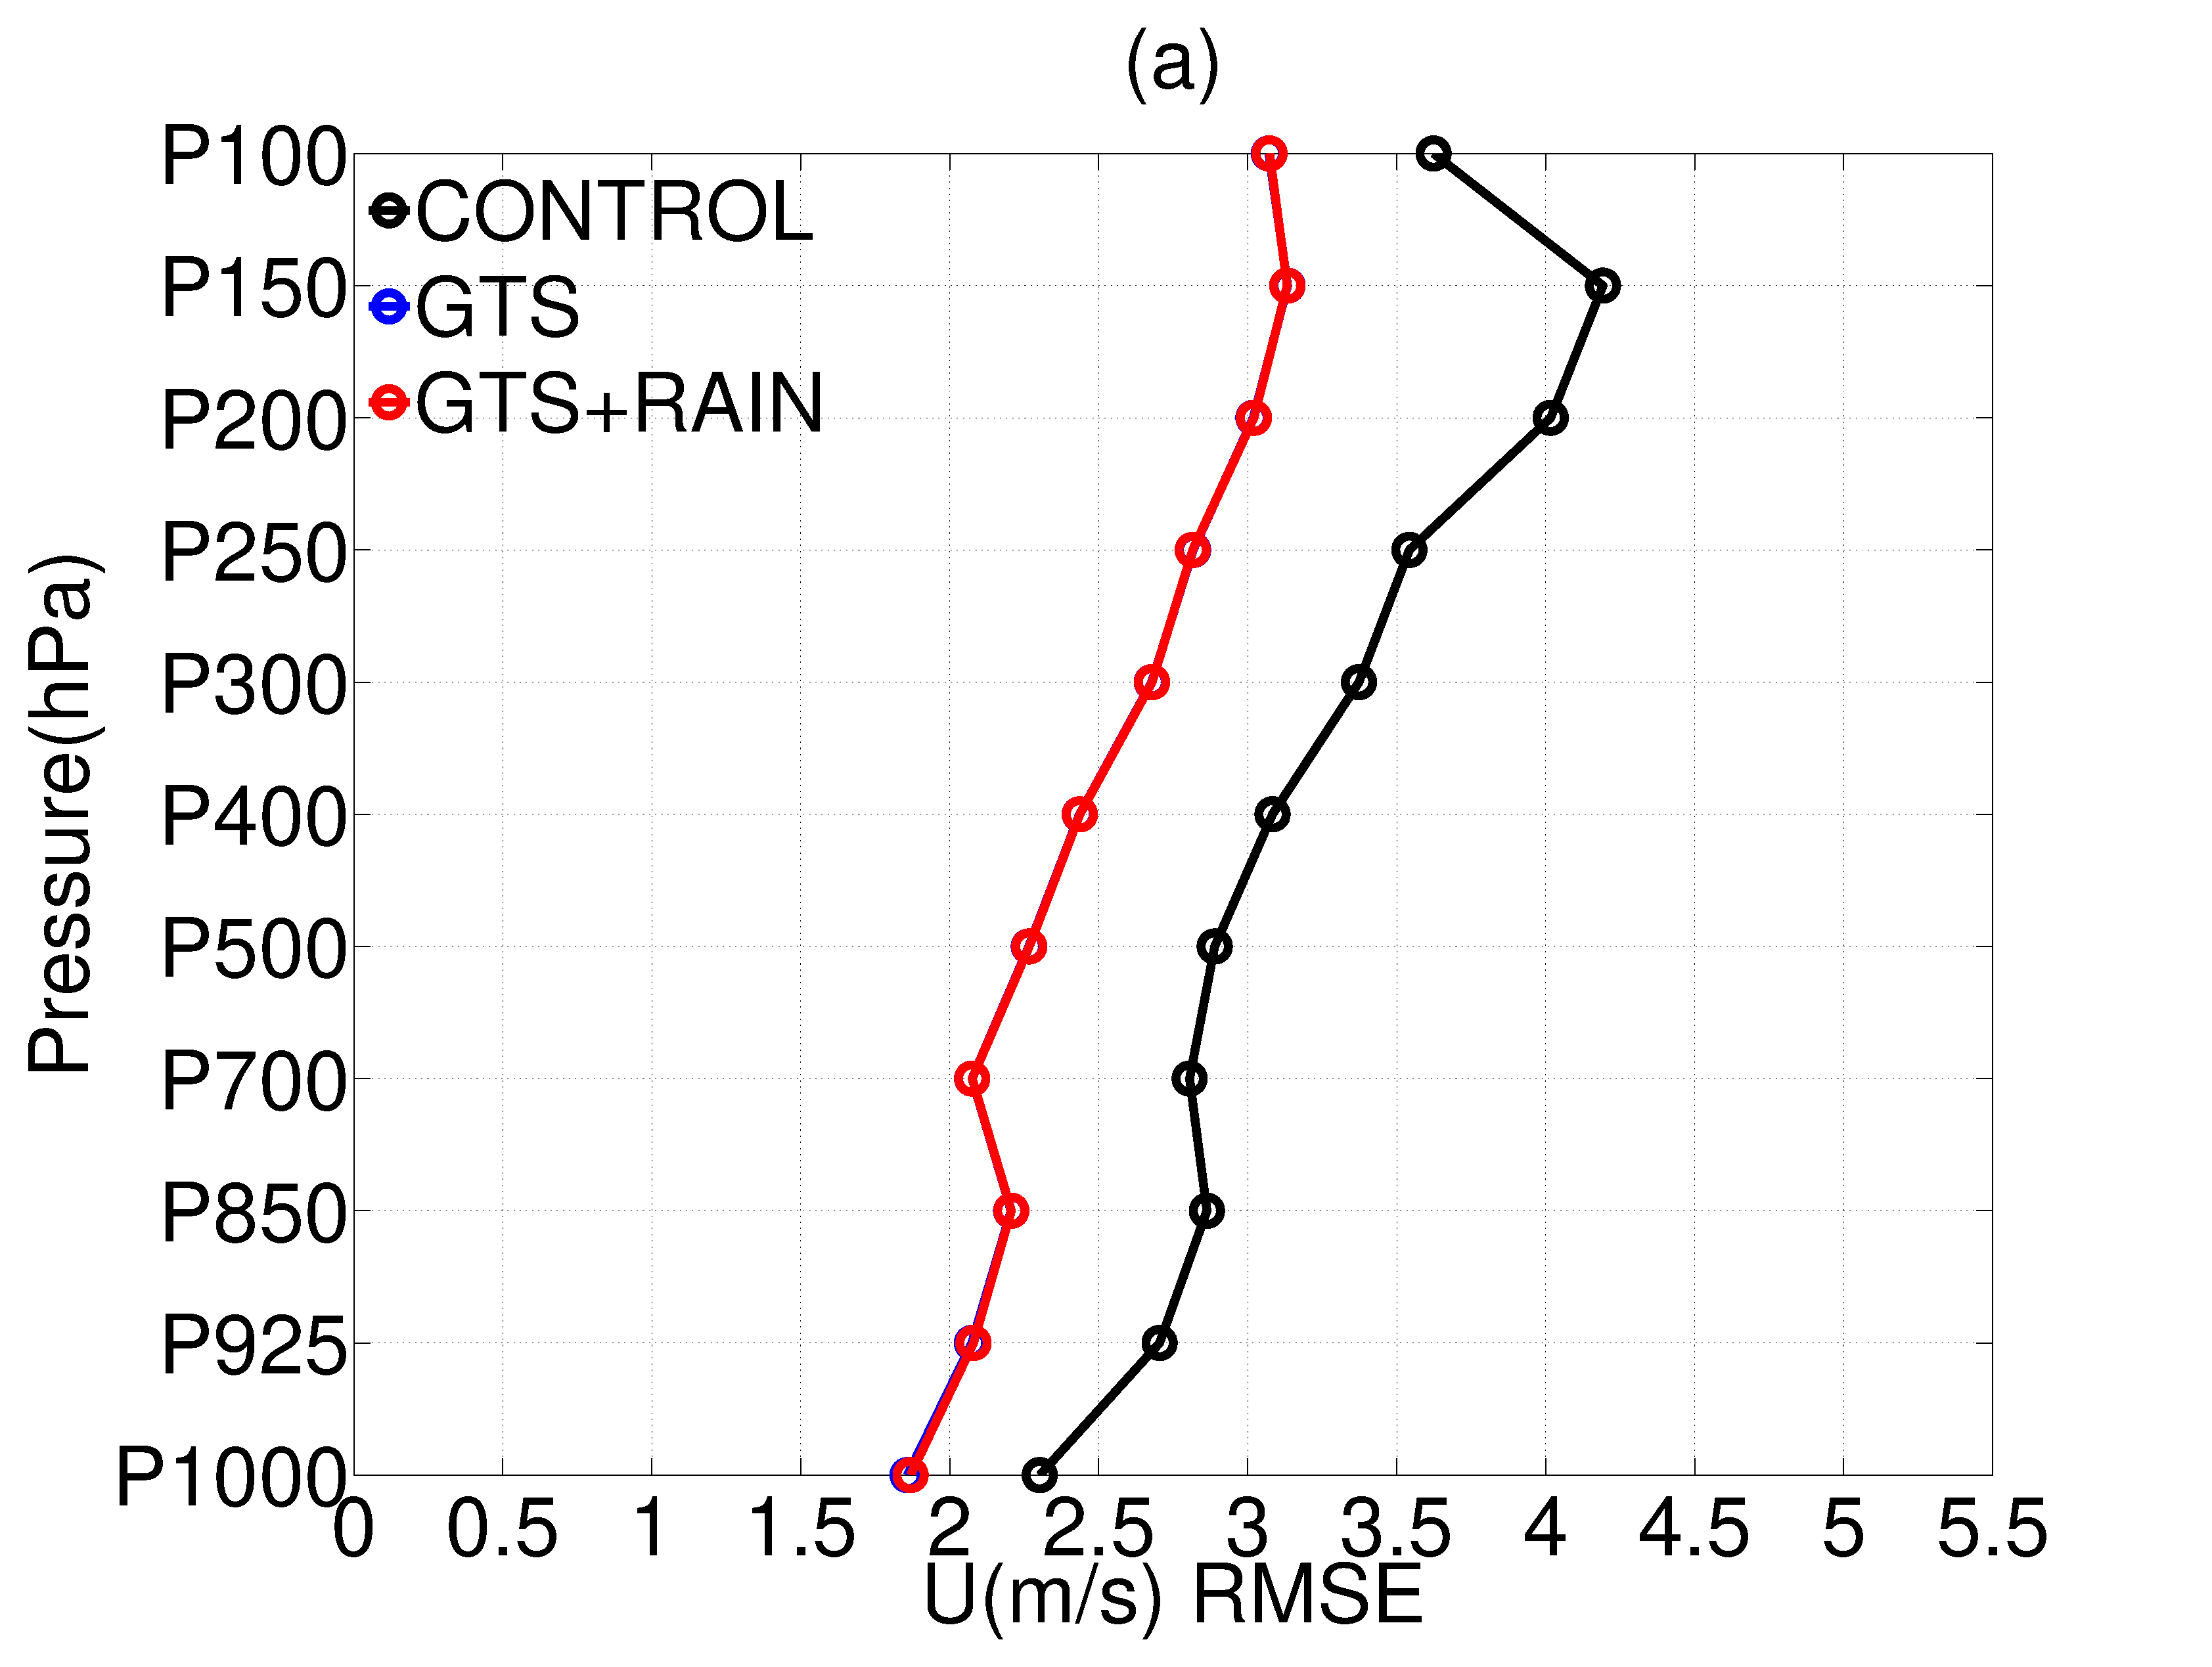
\includegraphics[width=0.5\linewidth]{./figures/u_00.eps}

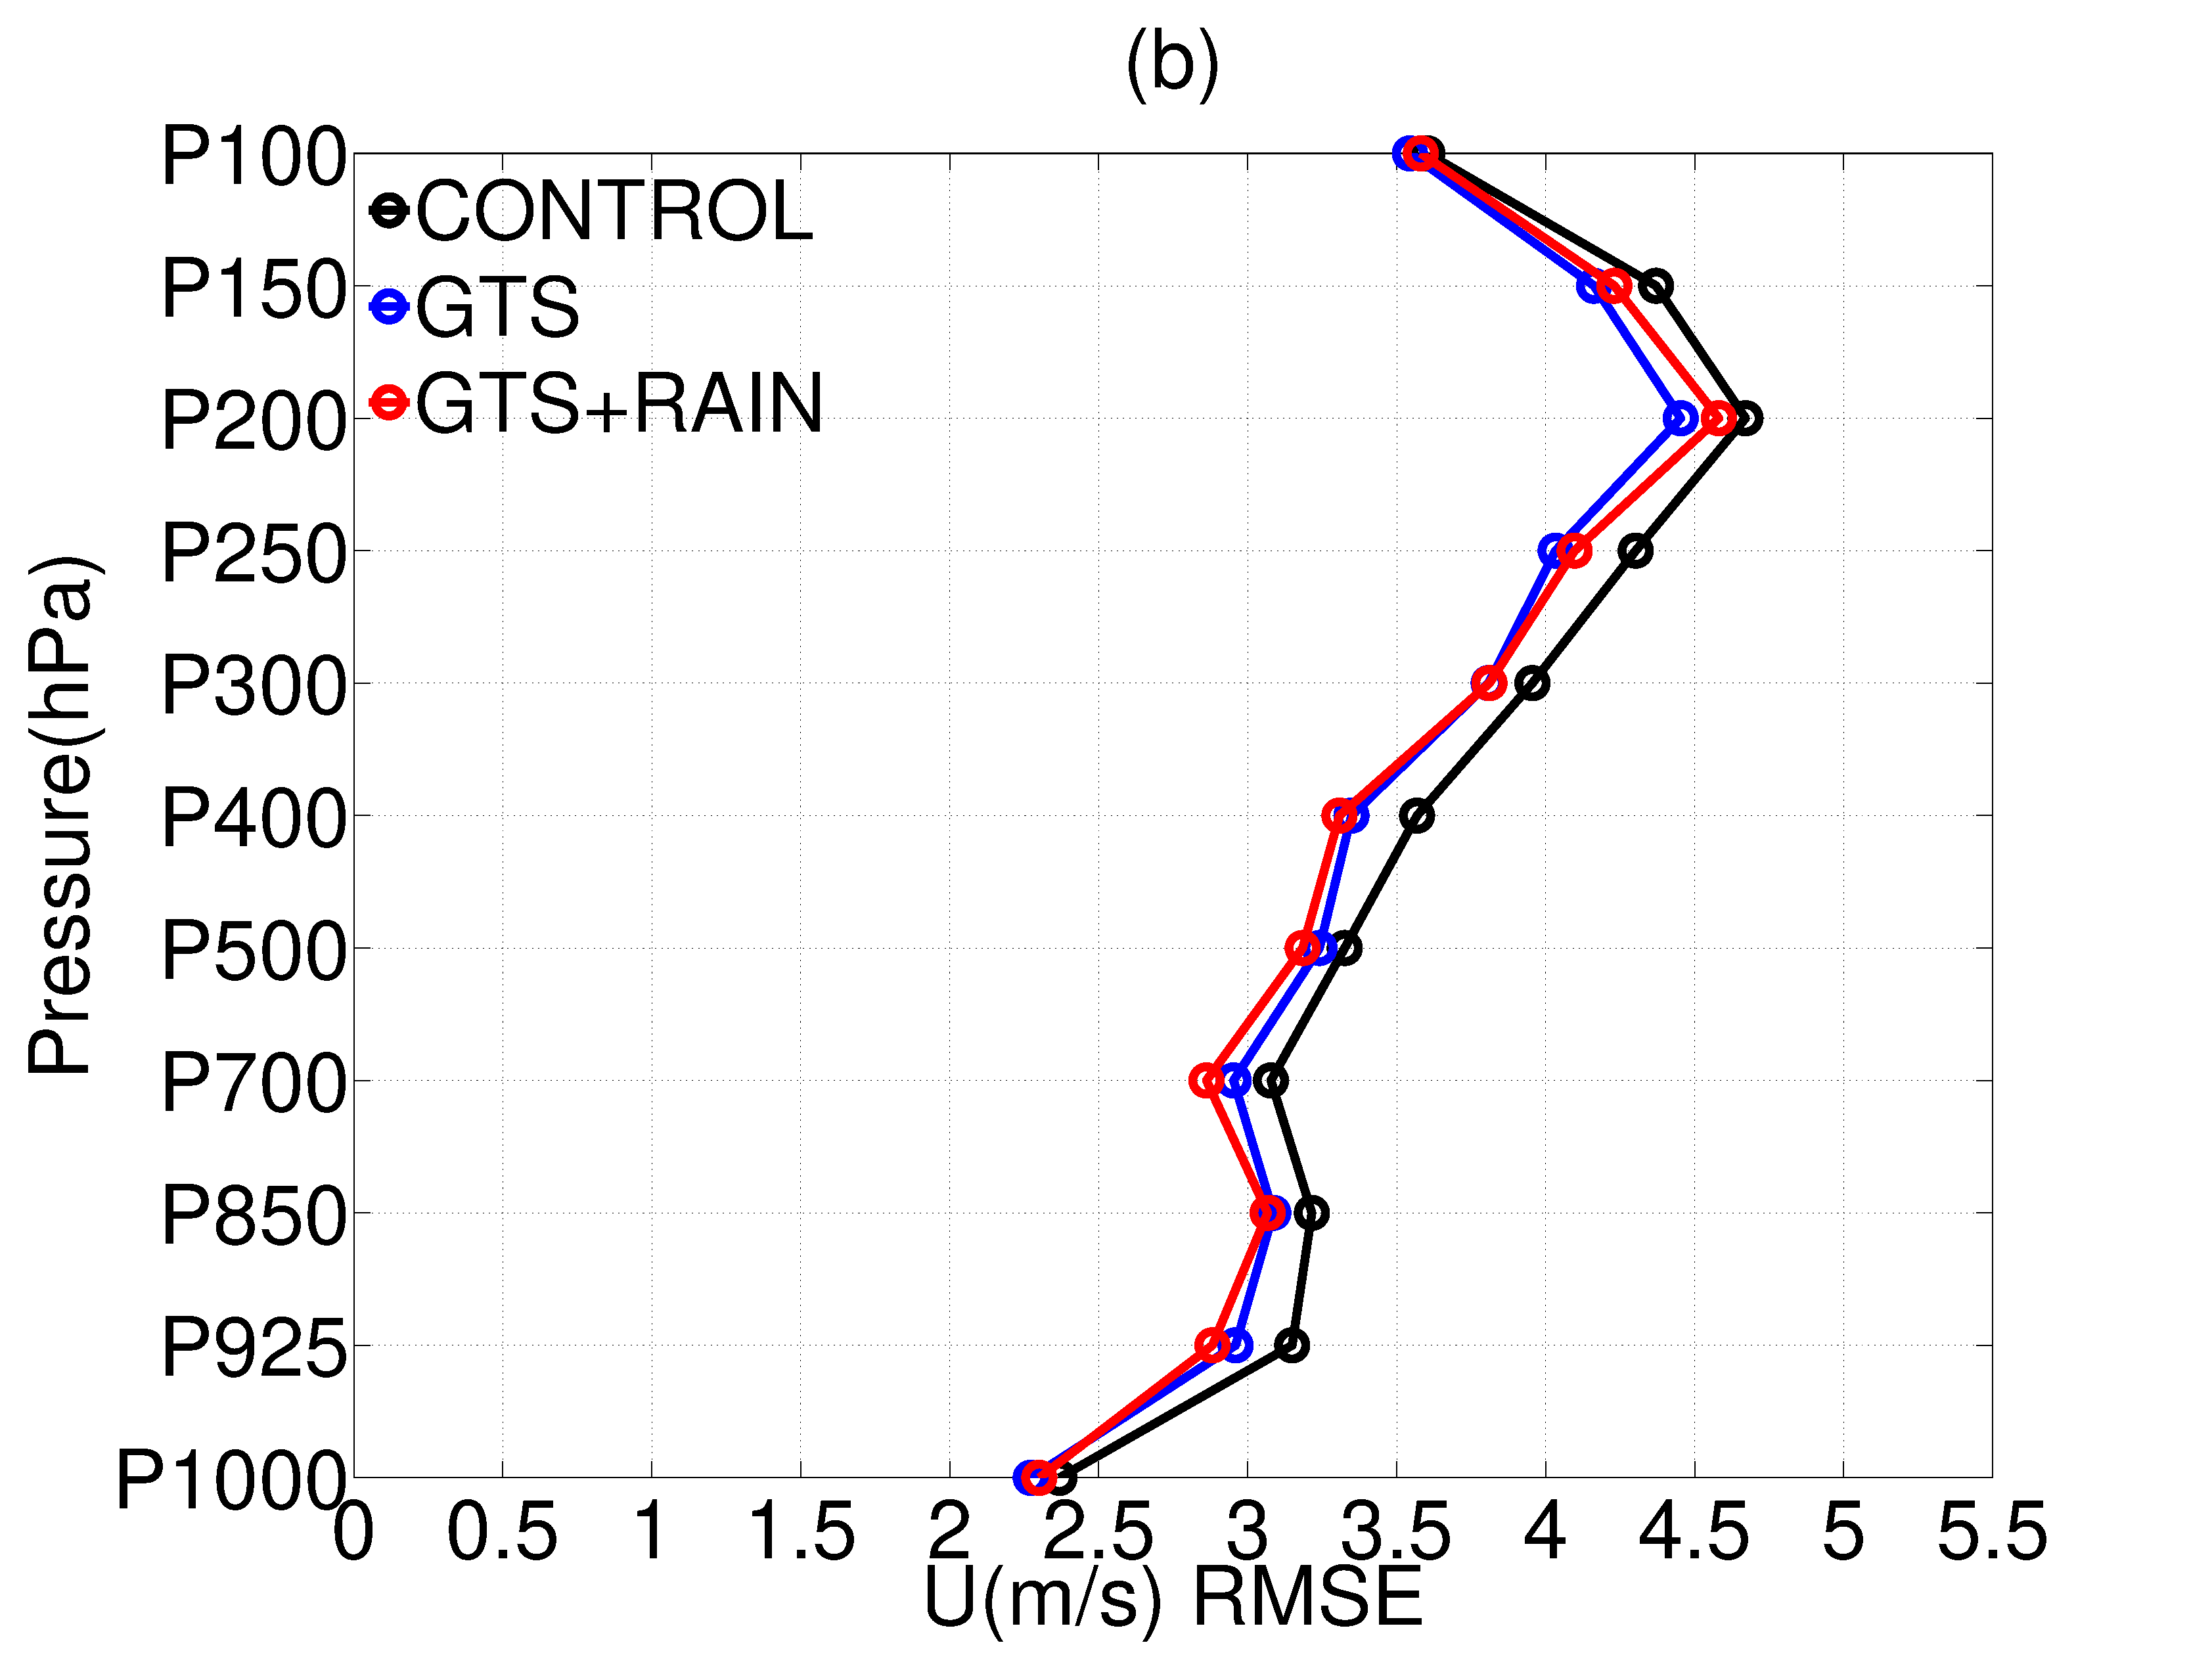
\includegraphics[width=0.5\linewidth]{./figures/u_12.eps}

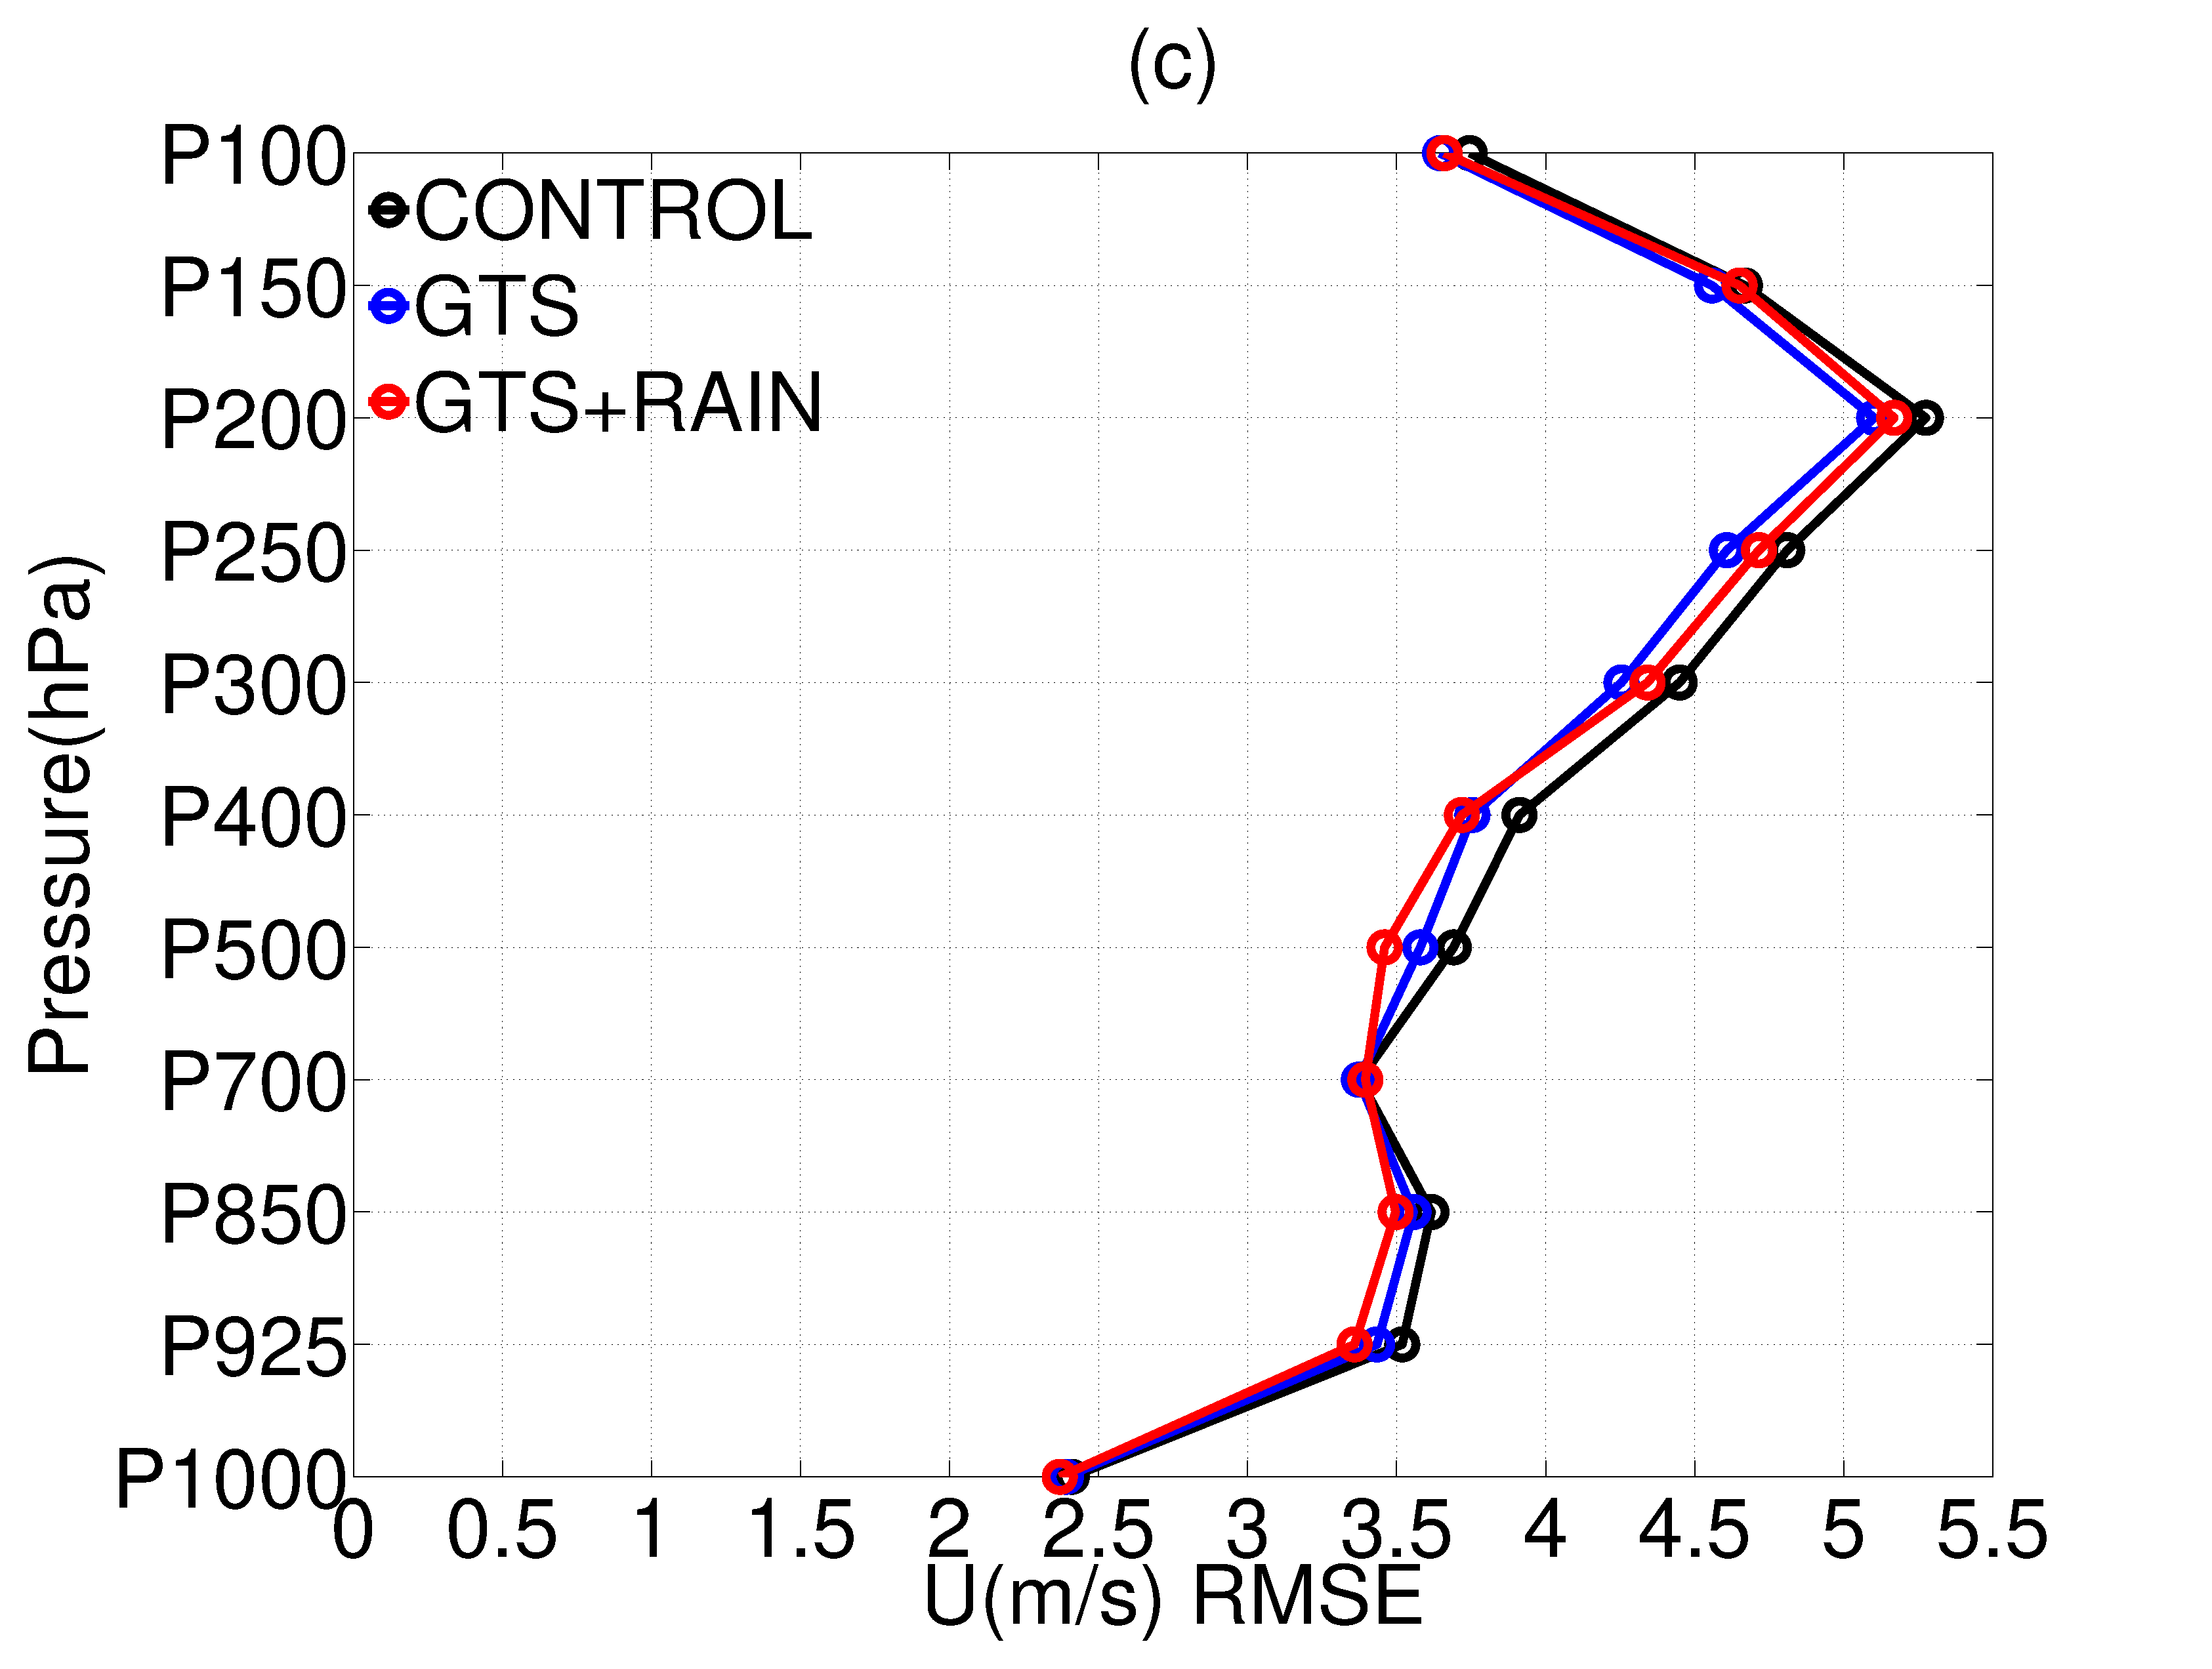
\includegraphics[width=0.5\linewidth]{./figures/u_24.eps}
\caption{Vertical profile of RMSE in U-component of the vector wind for experiments CONTROL, GTS and GTS+RAIN for analysis (a), 12h forecast(b) and 24h forecast(c) aggregated over 14-day period of cases verified against upper air sounding data.}\label{u_00}
\end{figure}

\newpage
\begin{figure}
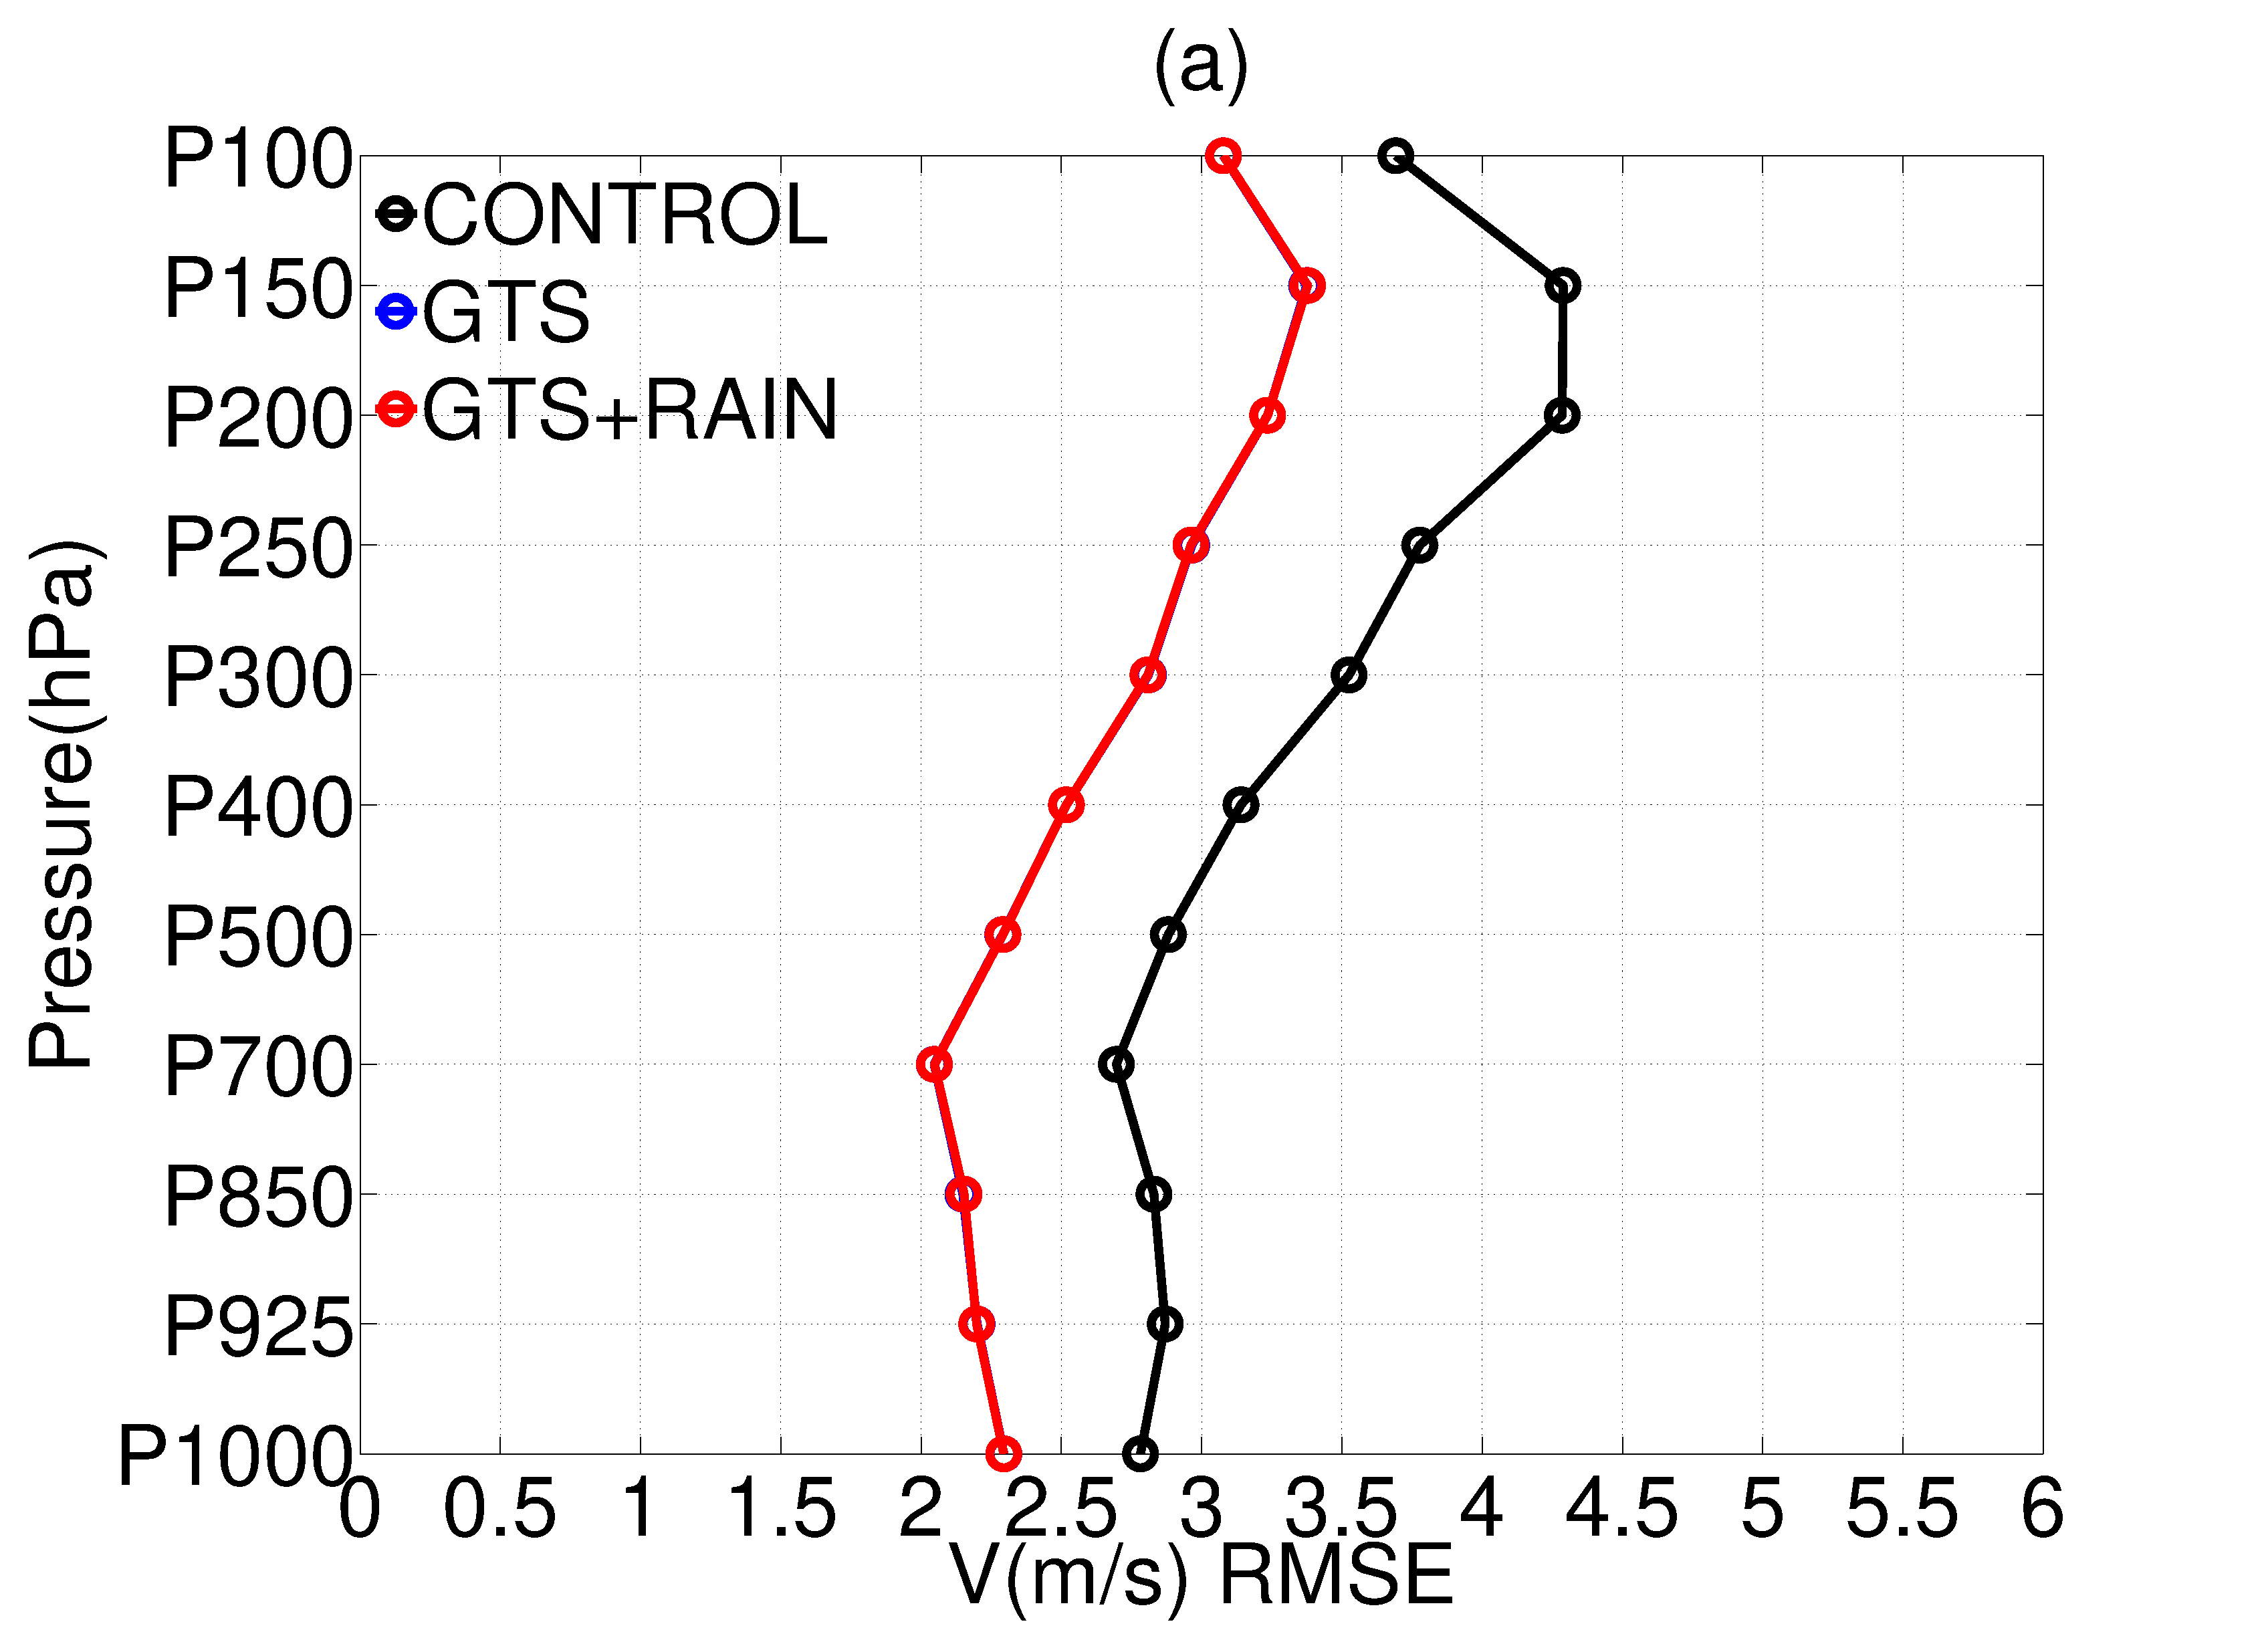
\includegraphics[width=0.5\linewidth]{./figures/v_00.eps}

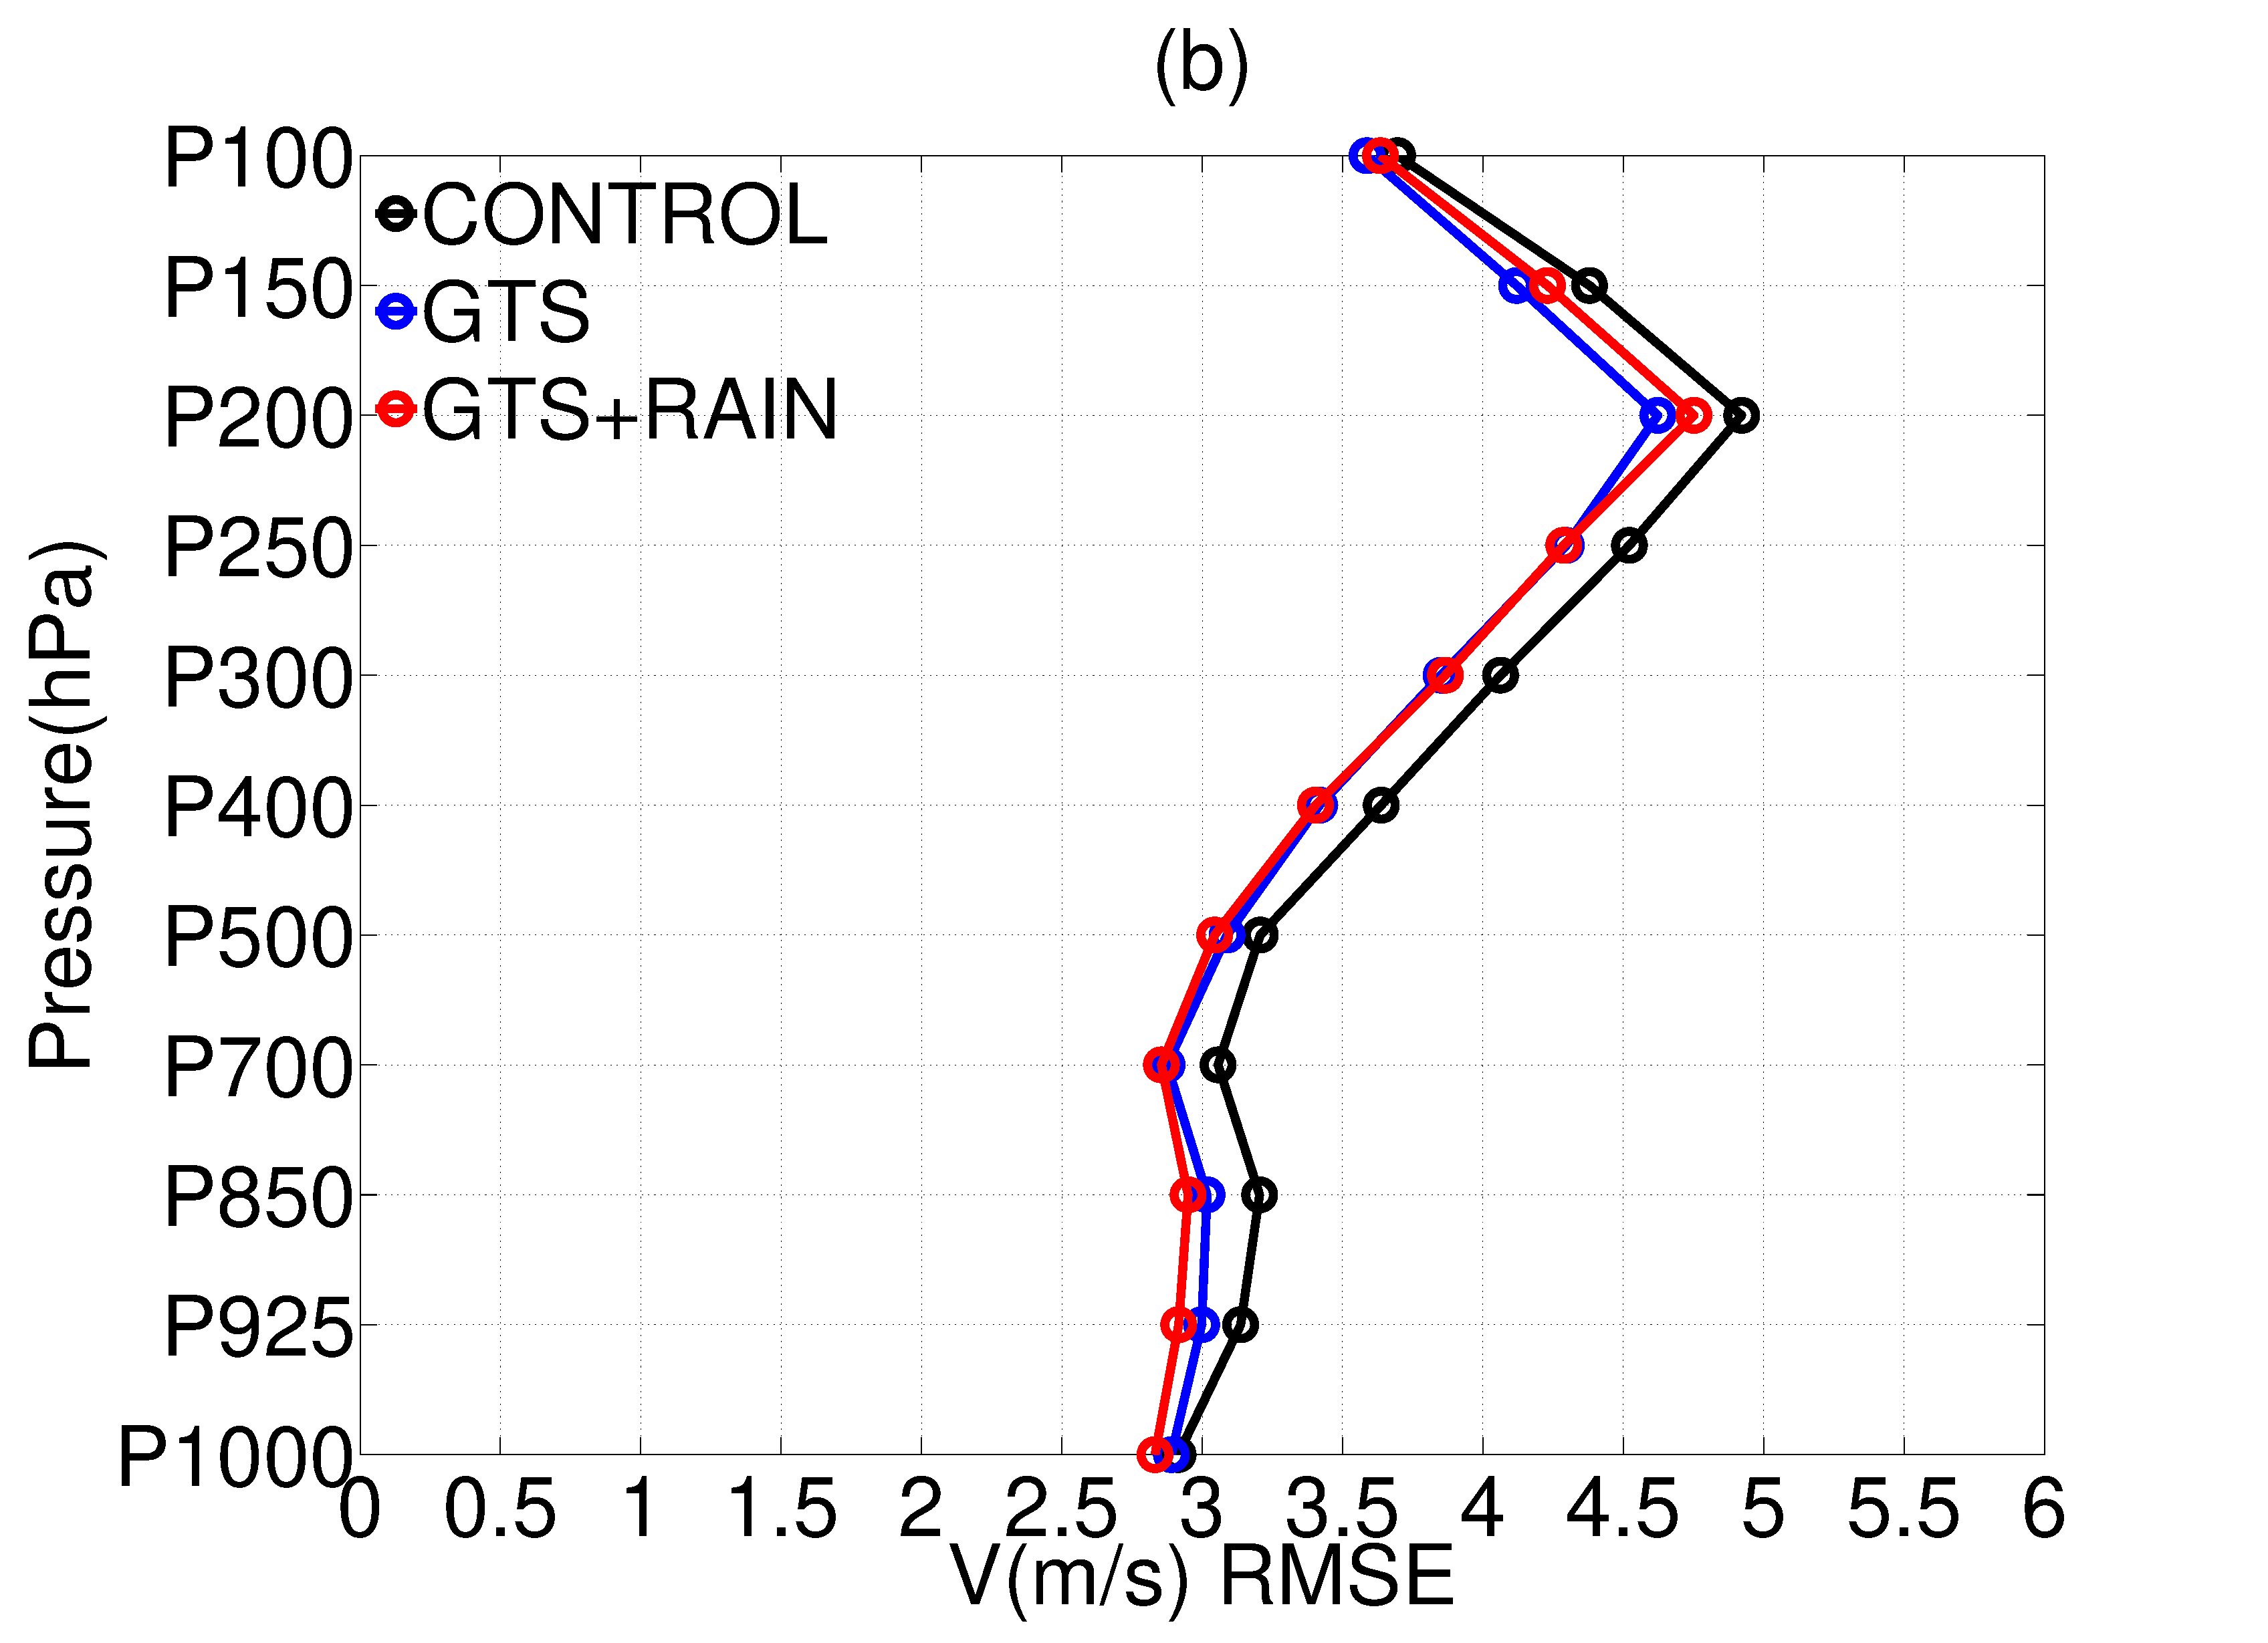
\includegraphics[width=0.5\linewidth]{./figures/v_12.eps}

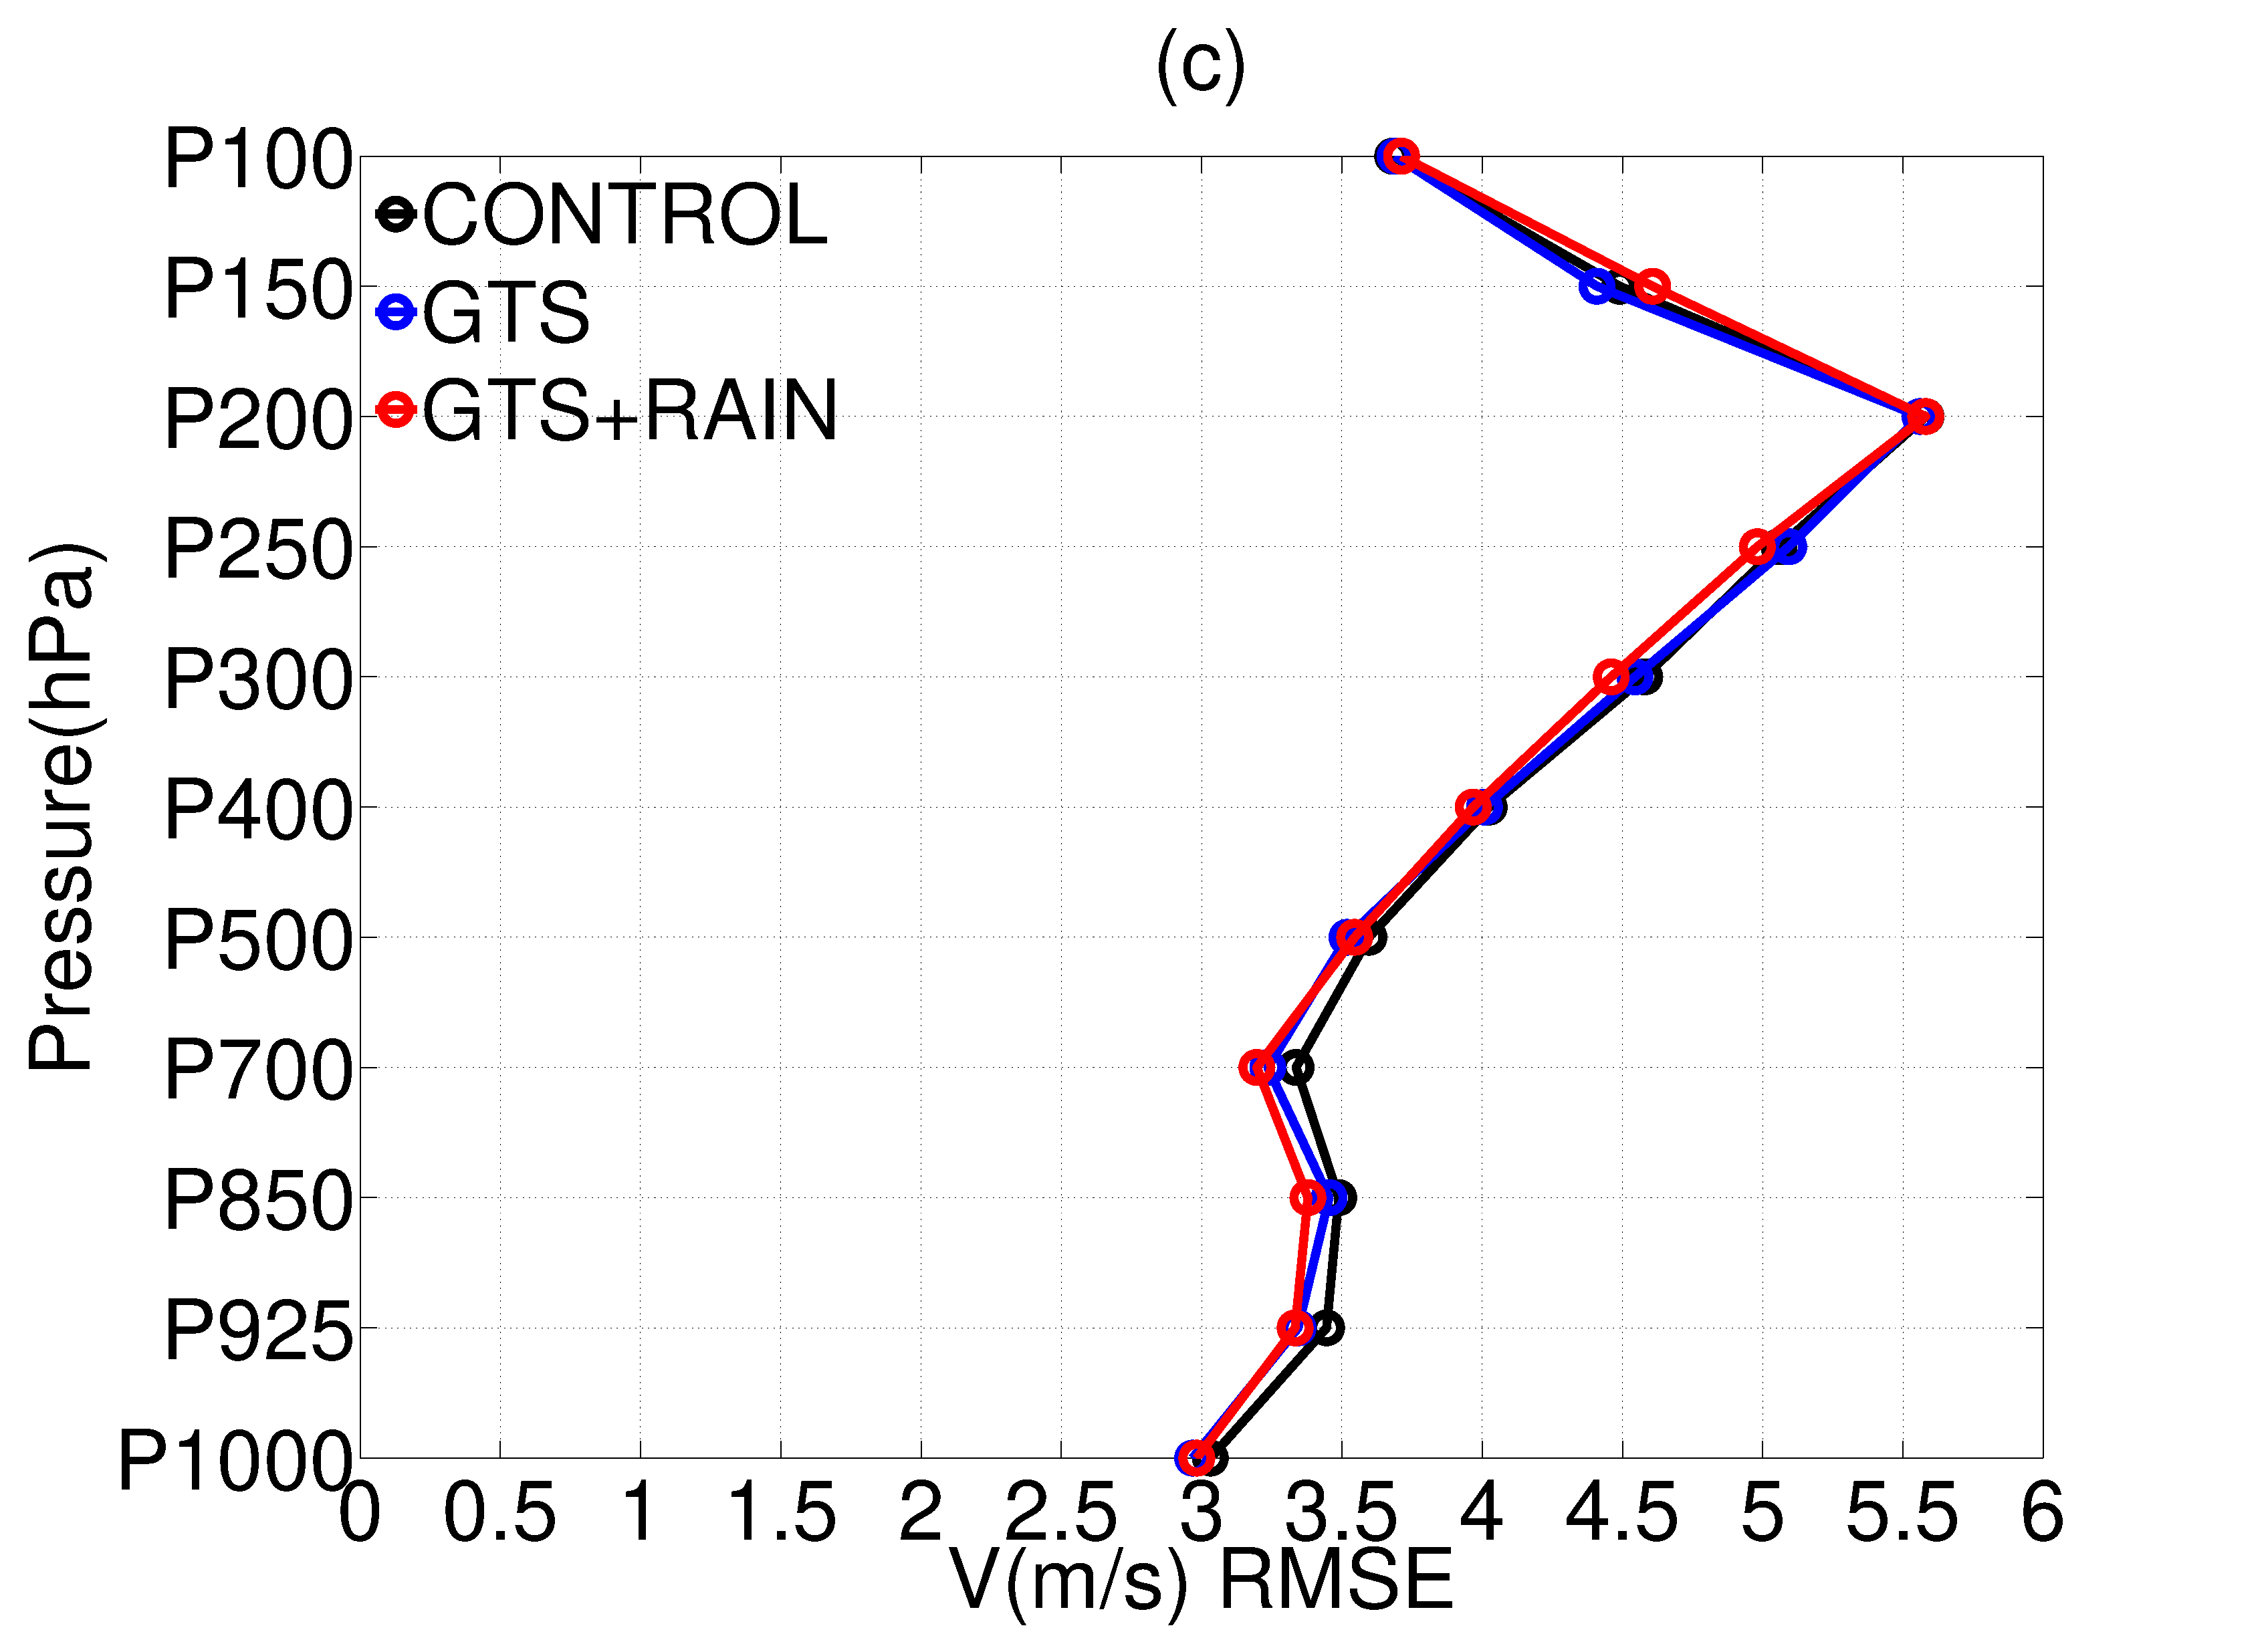
\includegraphics[width=0.5\linewidth]{./figures/v_24.eps}
\caption{Same as Figure 1 but for V-component of the vector wind. }\label{v_00}
\end{figure}

\newpage
\begin{figure}
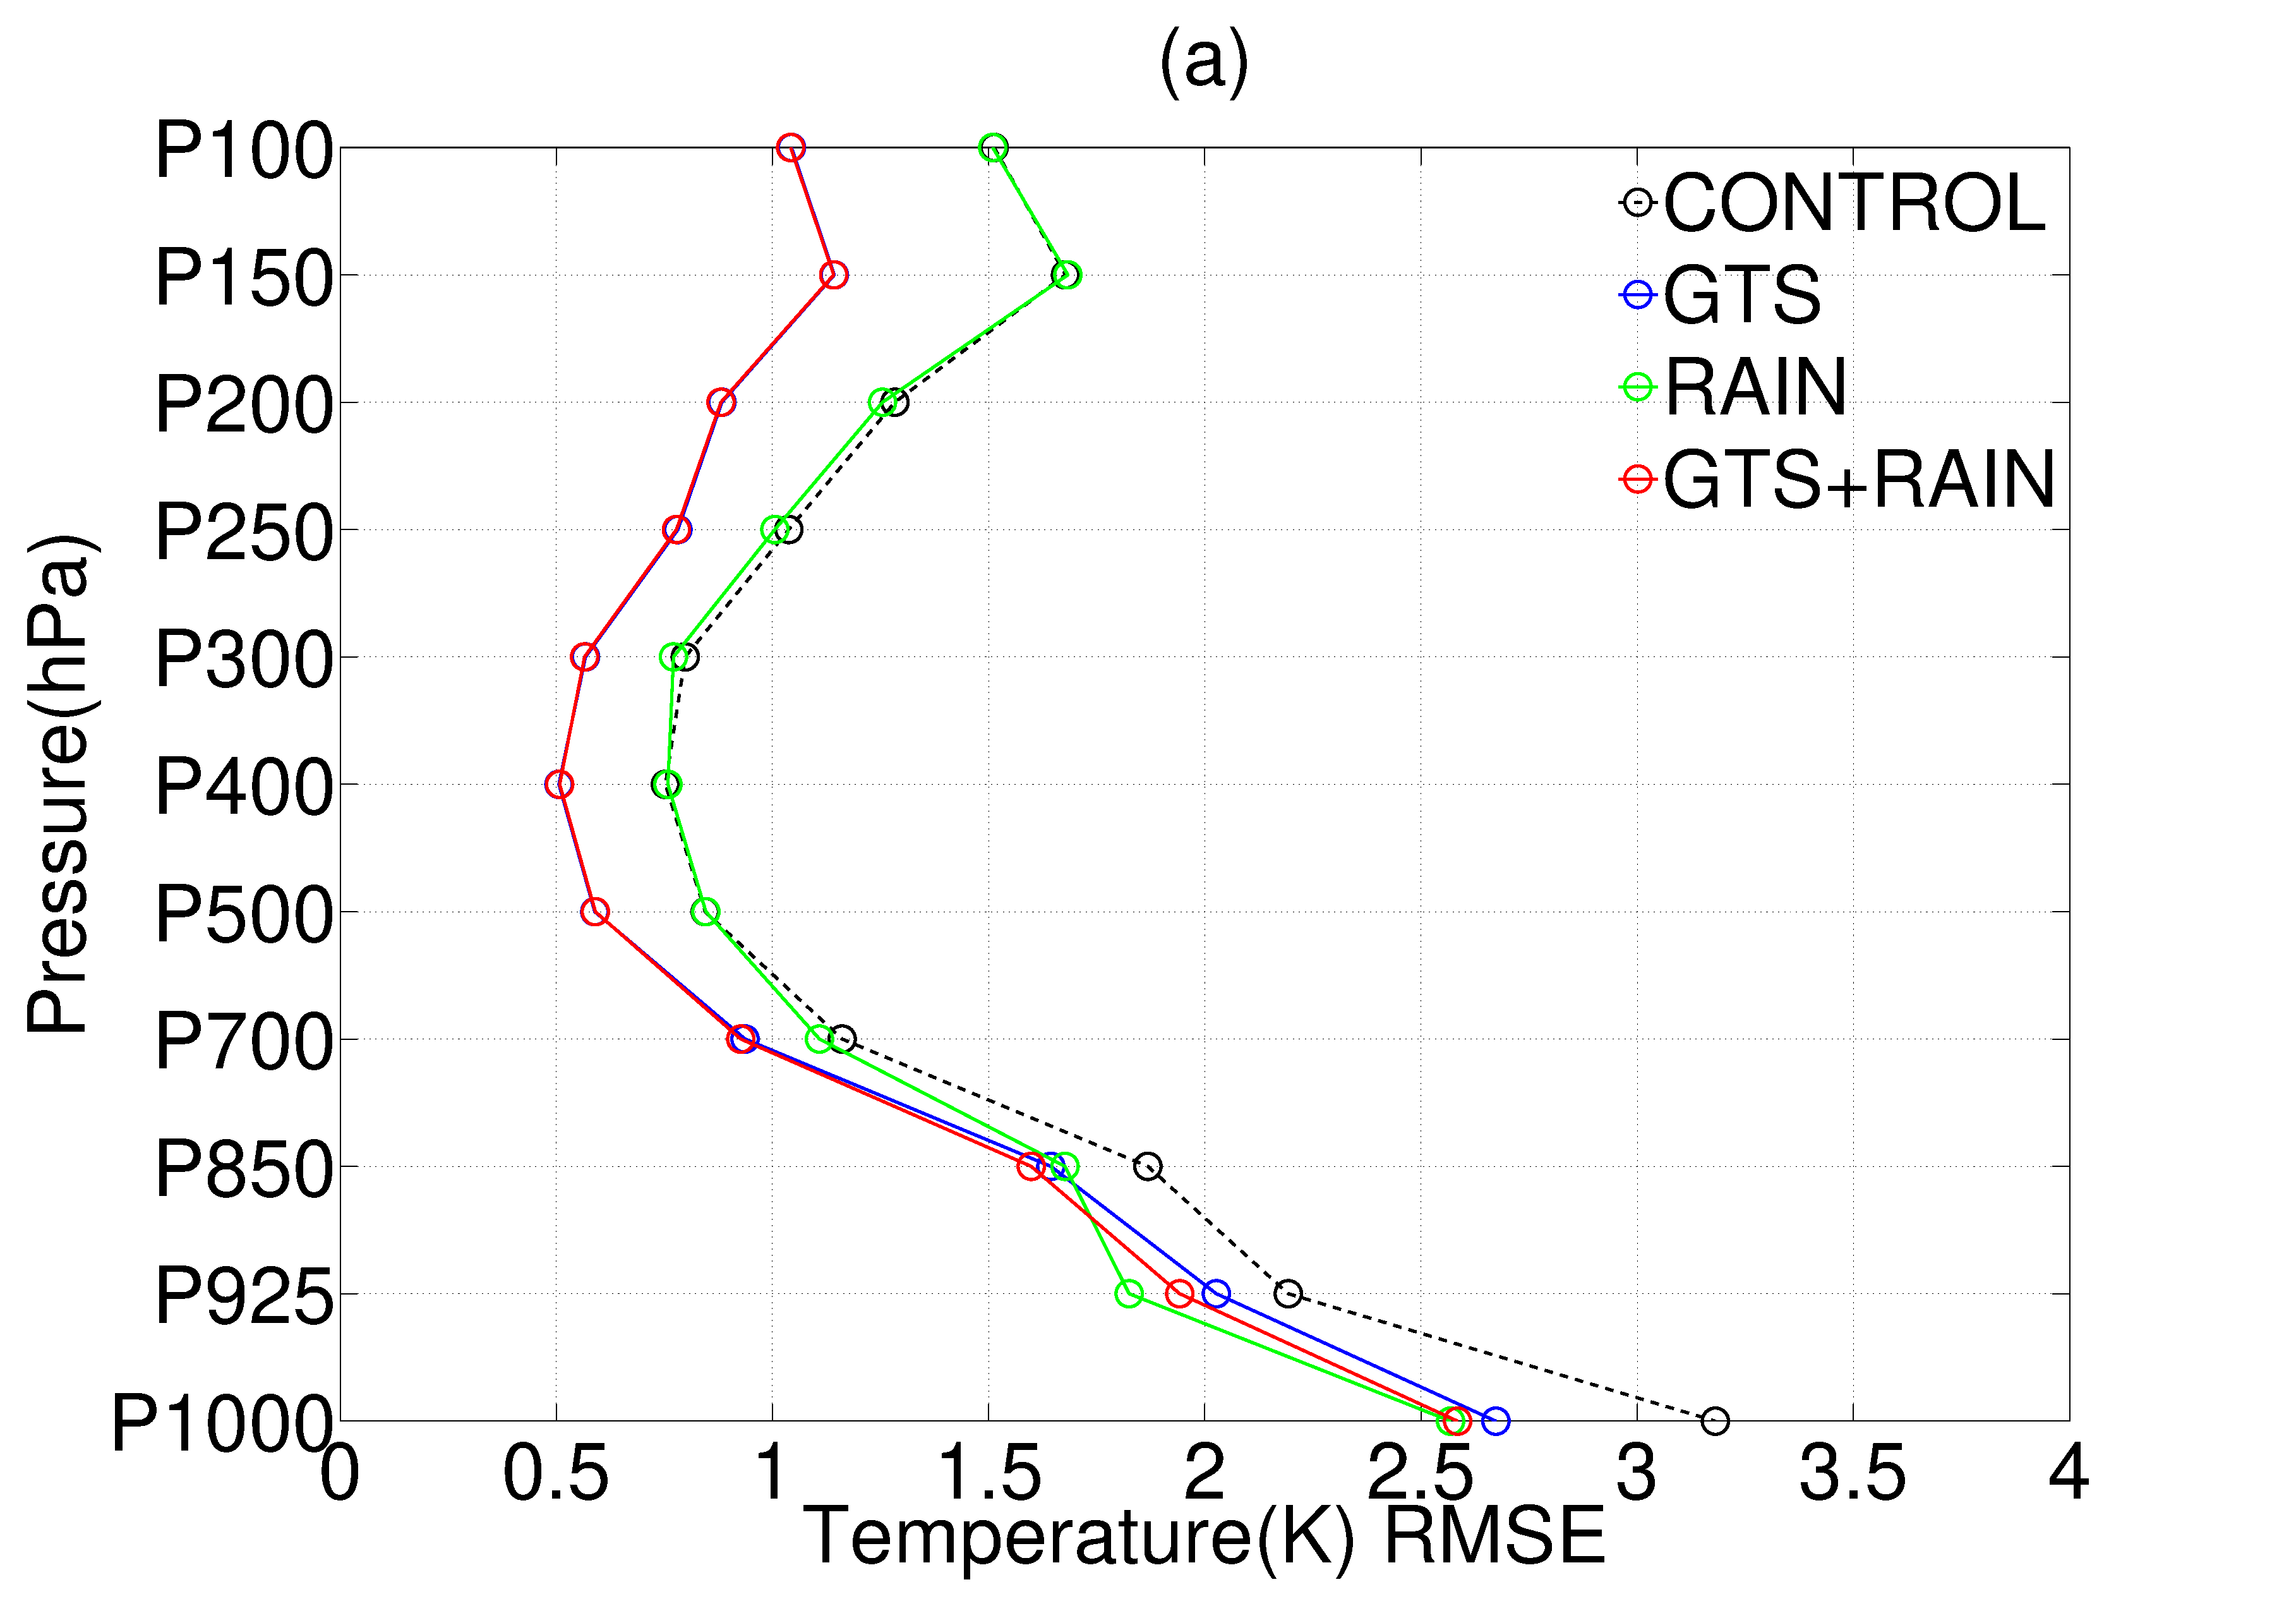
\includegraphics[width=0.5\linewidth]{./figures/tmp_00.eps}

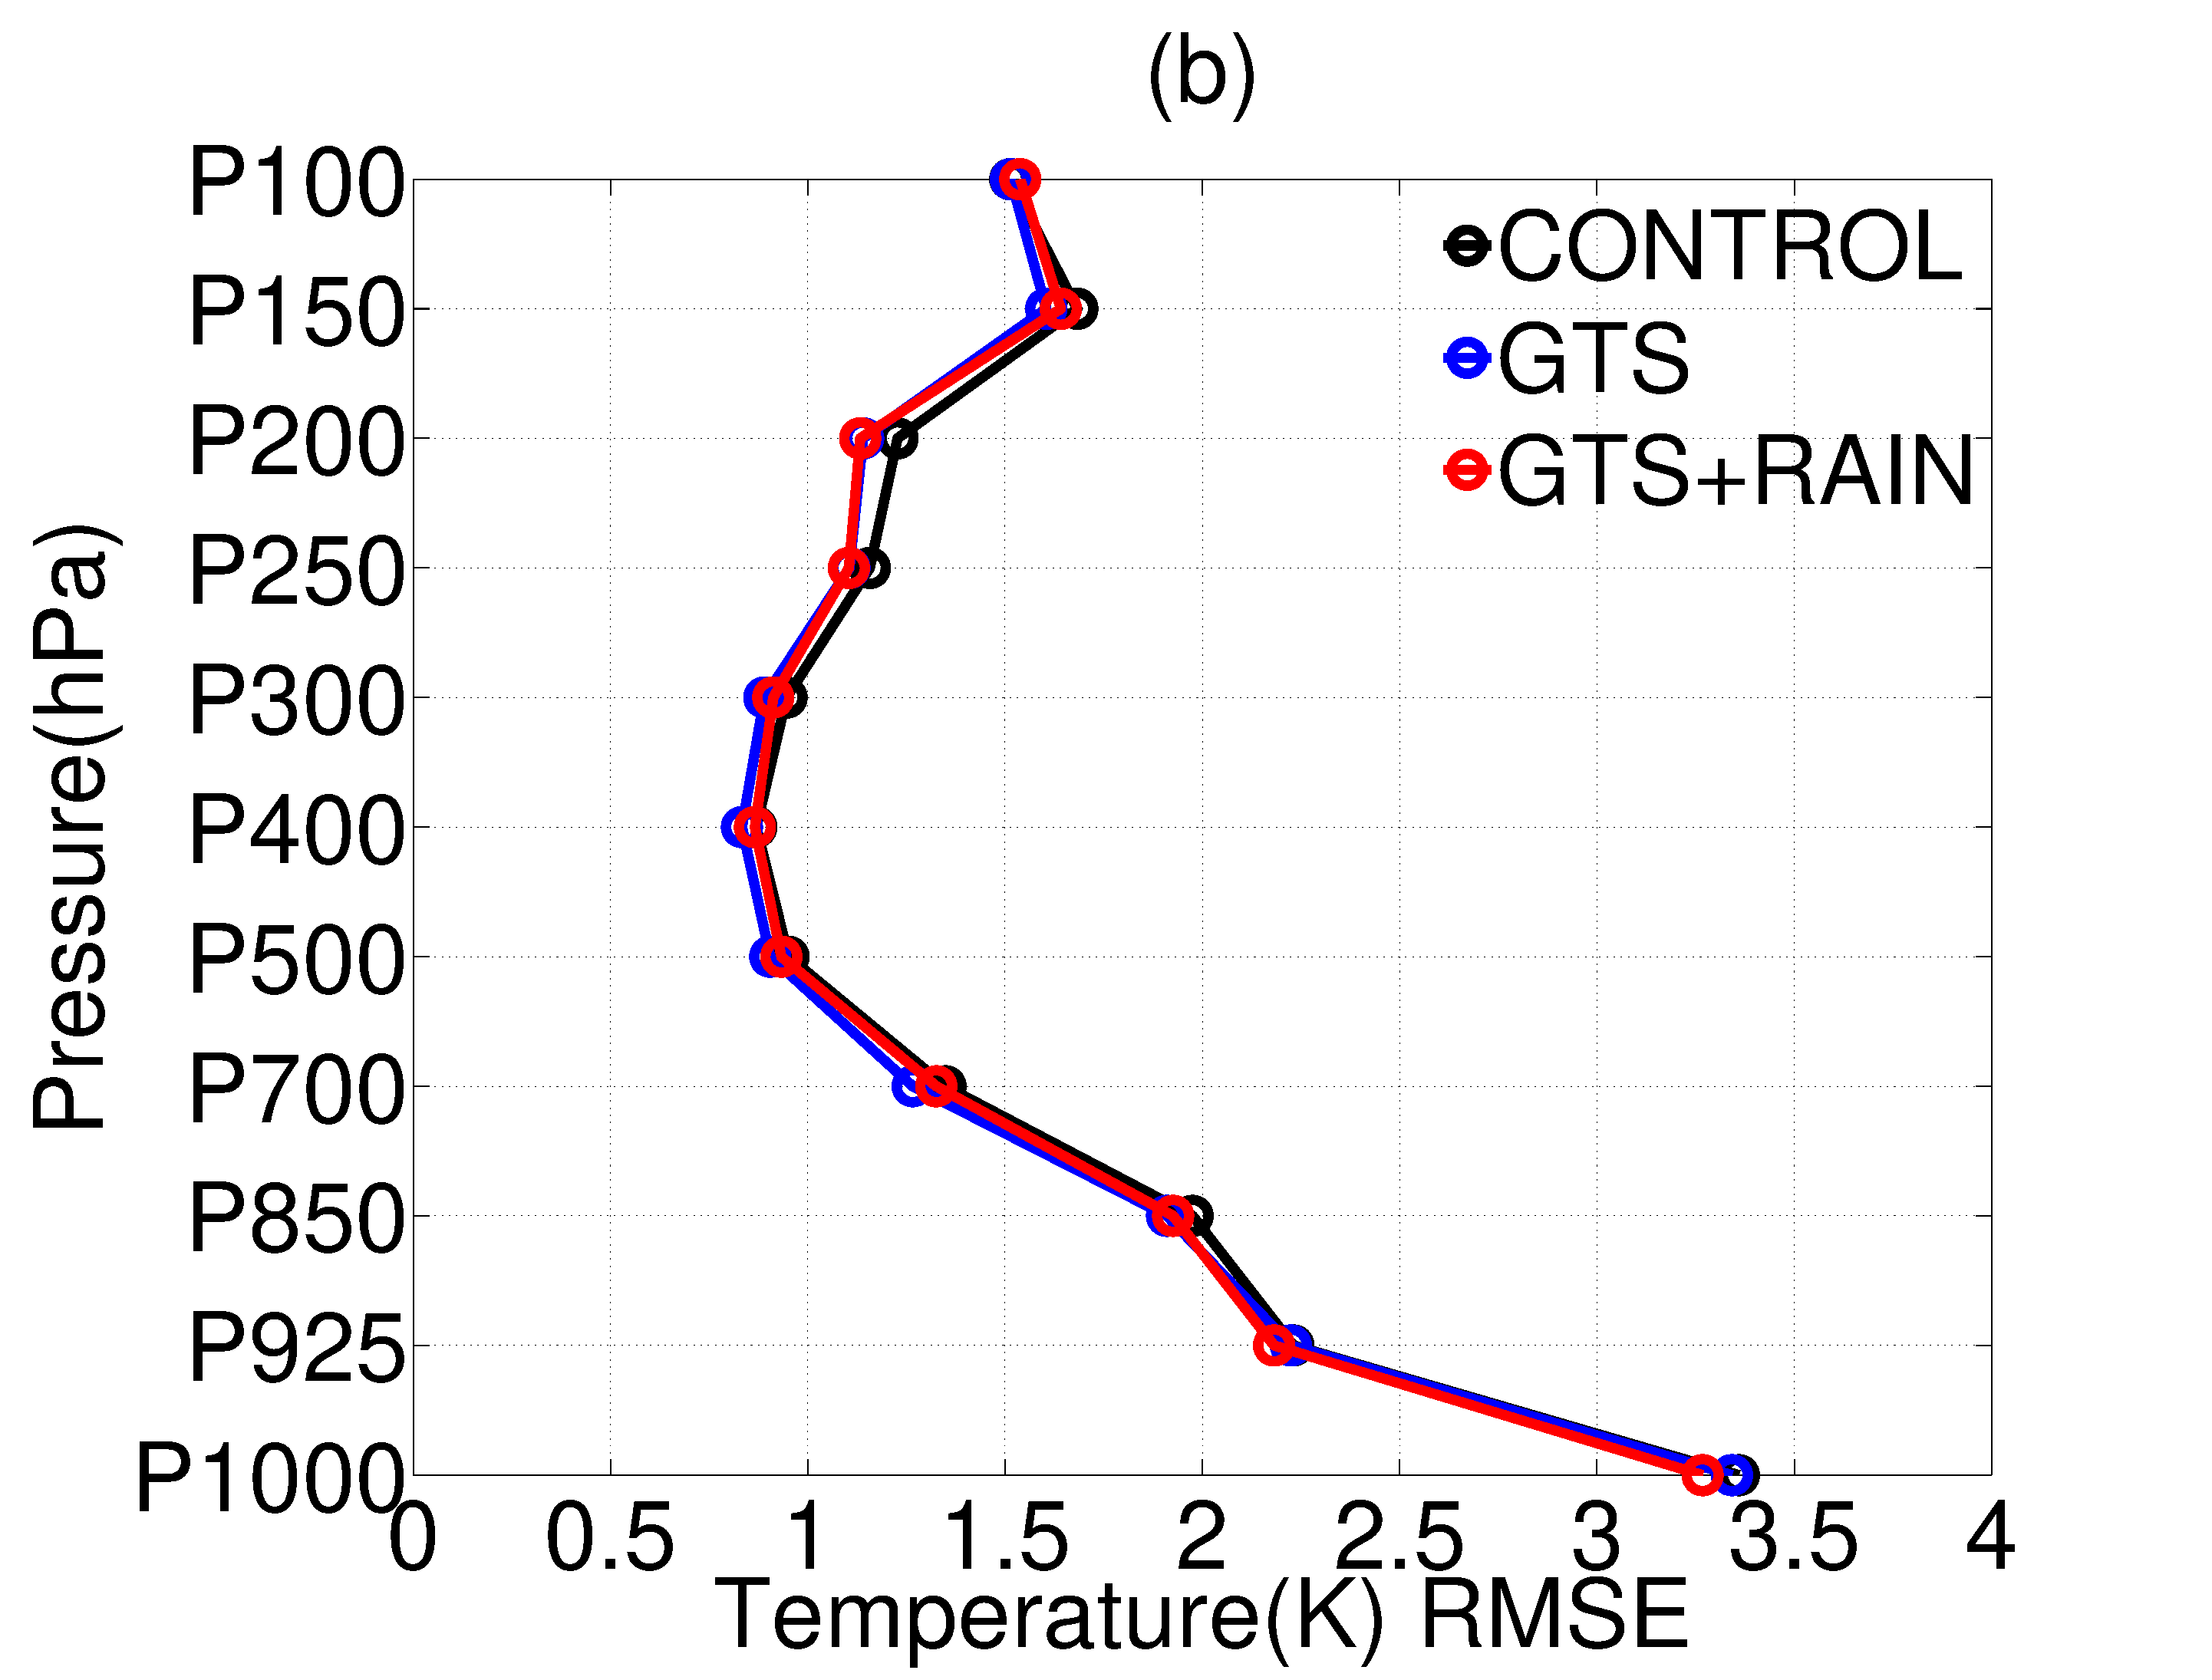
\includegraphics[width=0.5\linewidth]{./figures/tmp_12.eps}

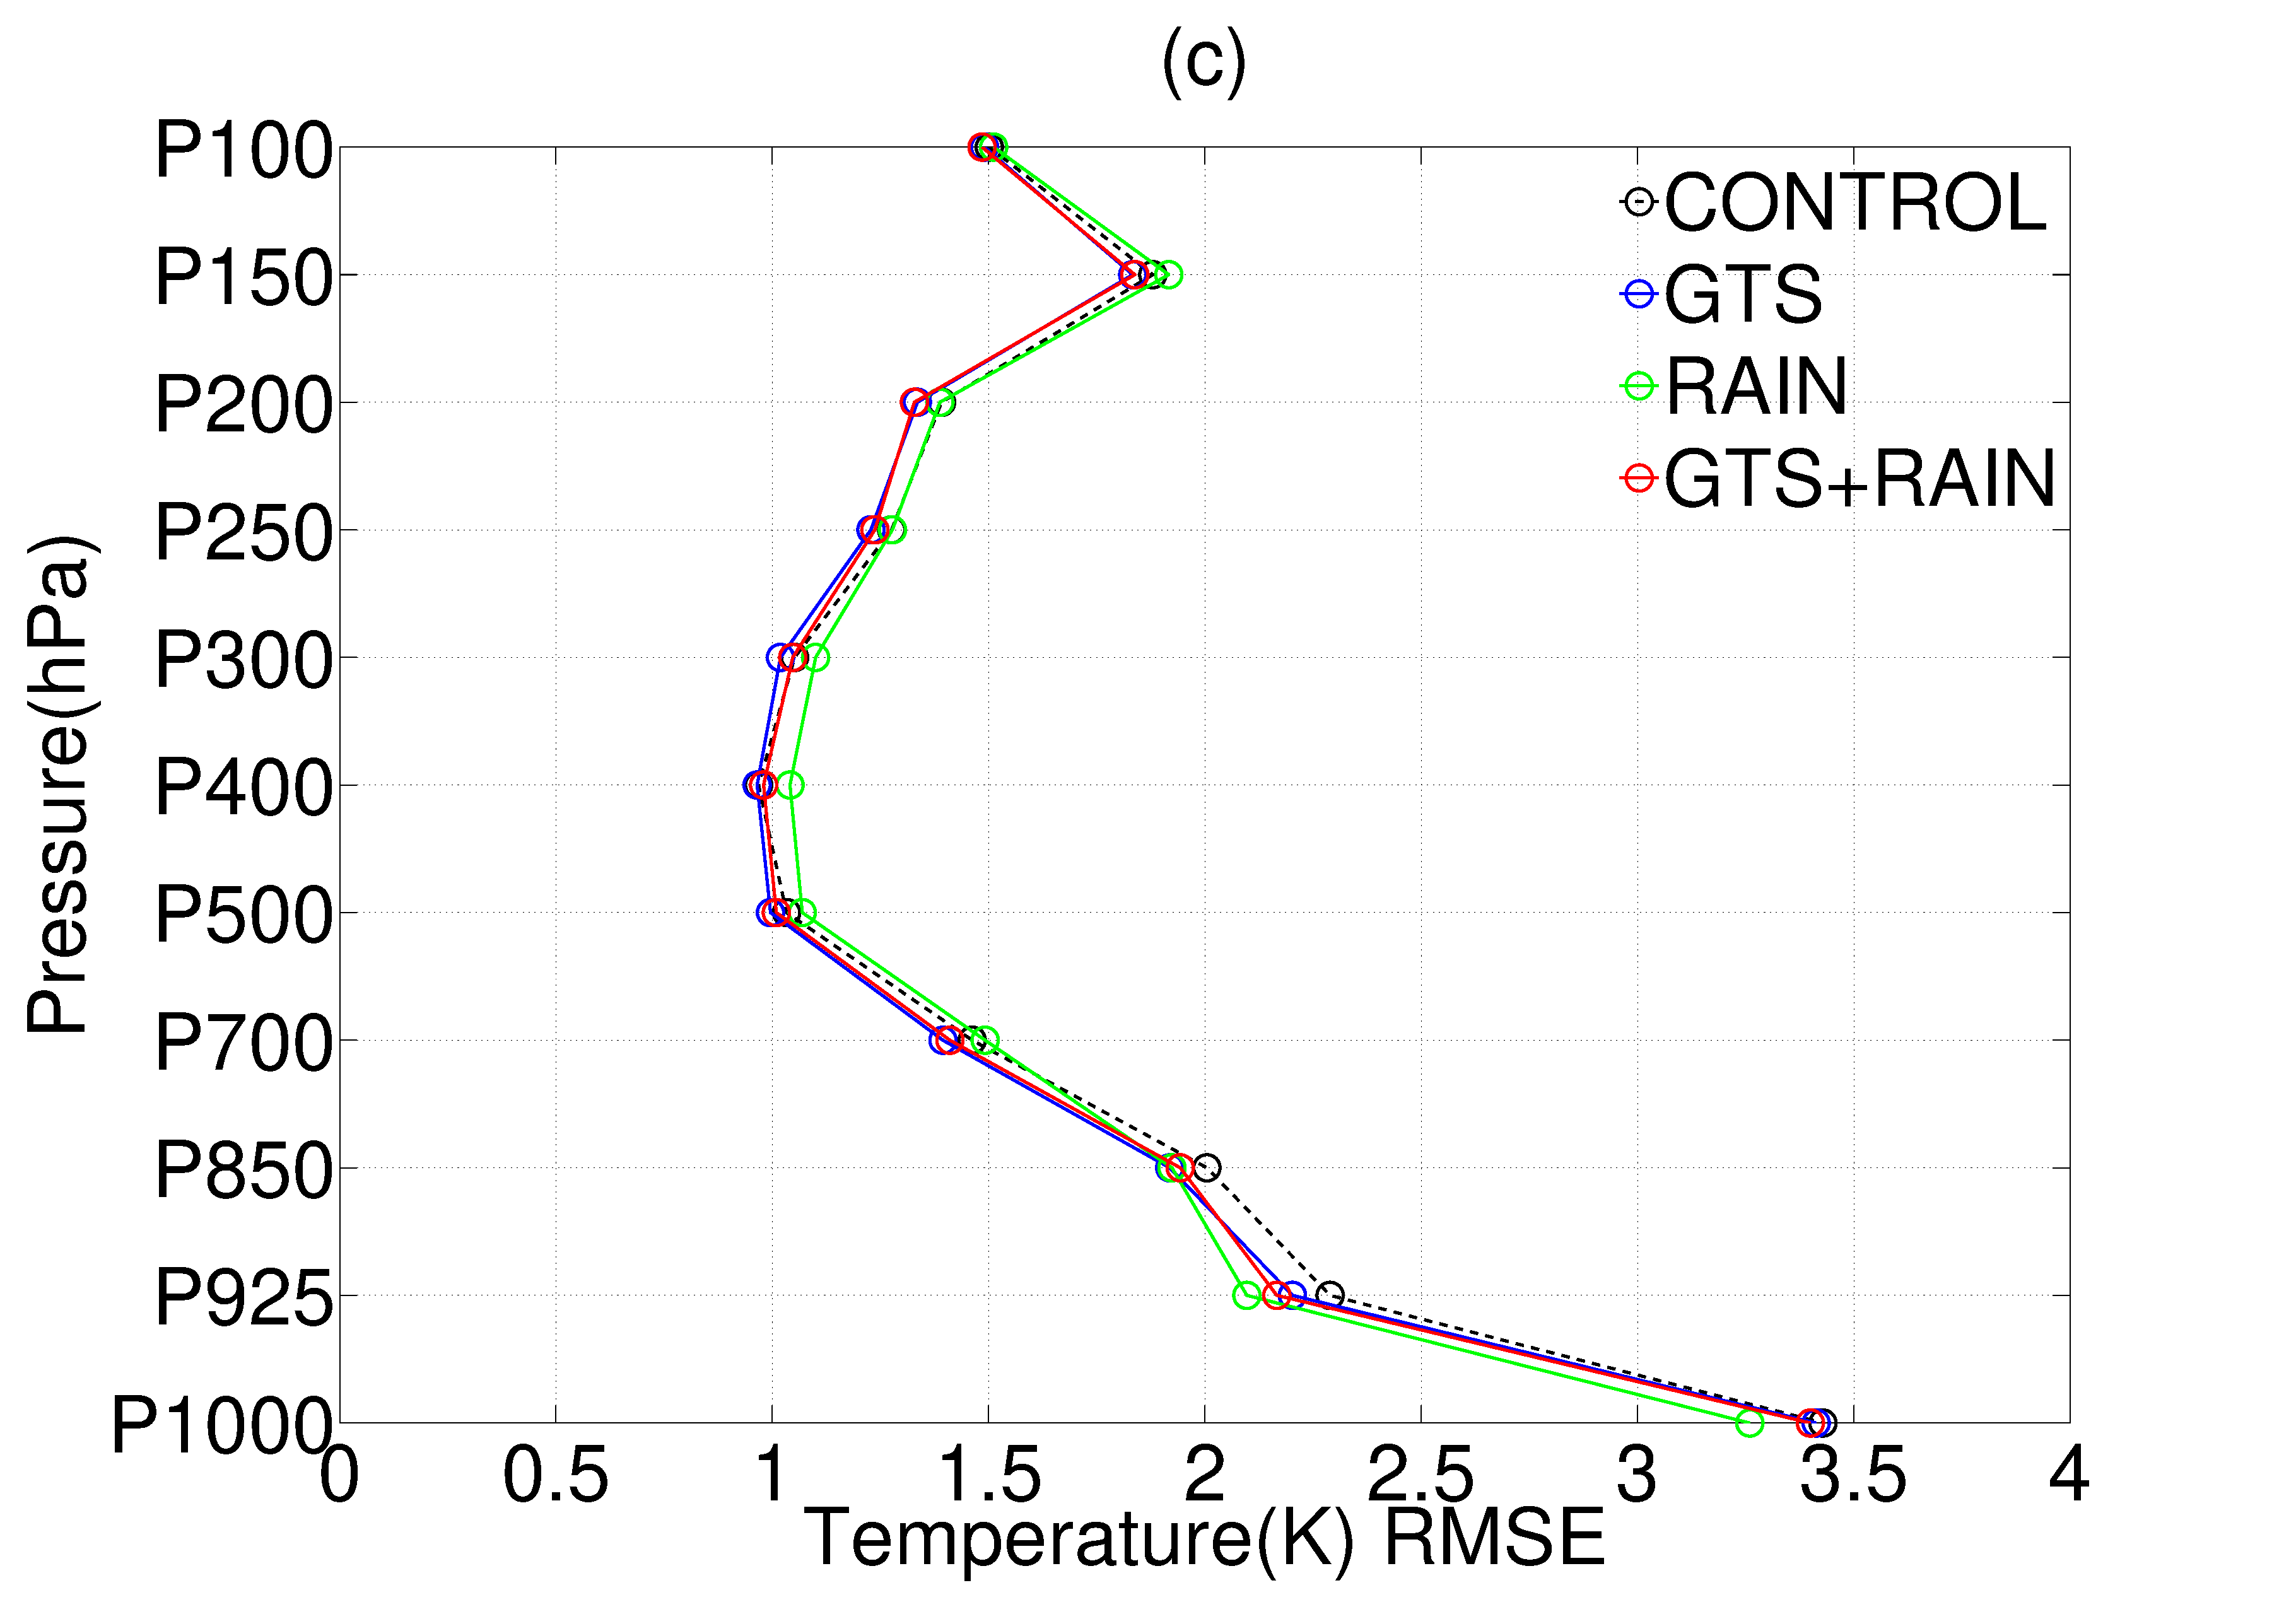
\includegraphics[width=0.5\linewidth]{./figures/tmp_24.eps}
\caption{Same as Figure 1 but for temperature. }\label{tmp_00}
\end{figure}

\newpage
\begin{figure}
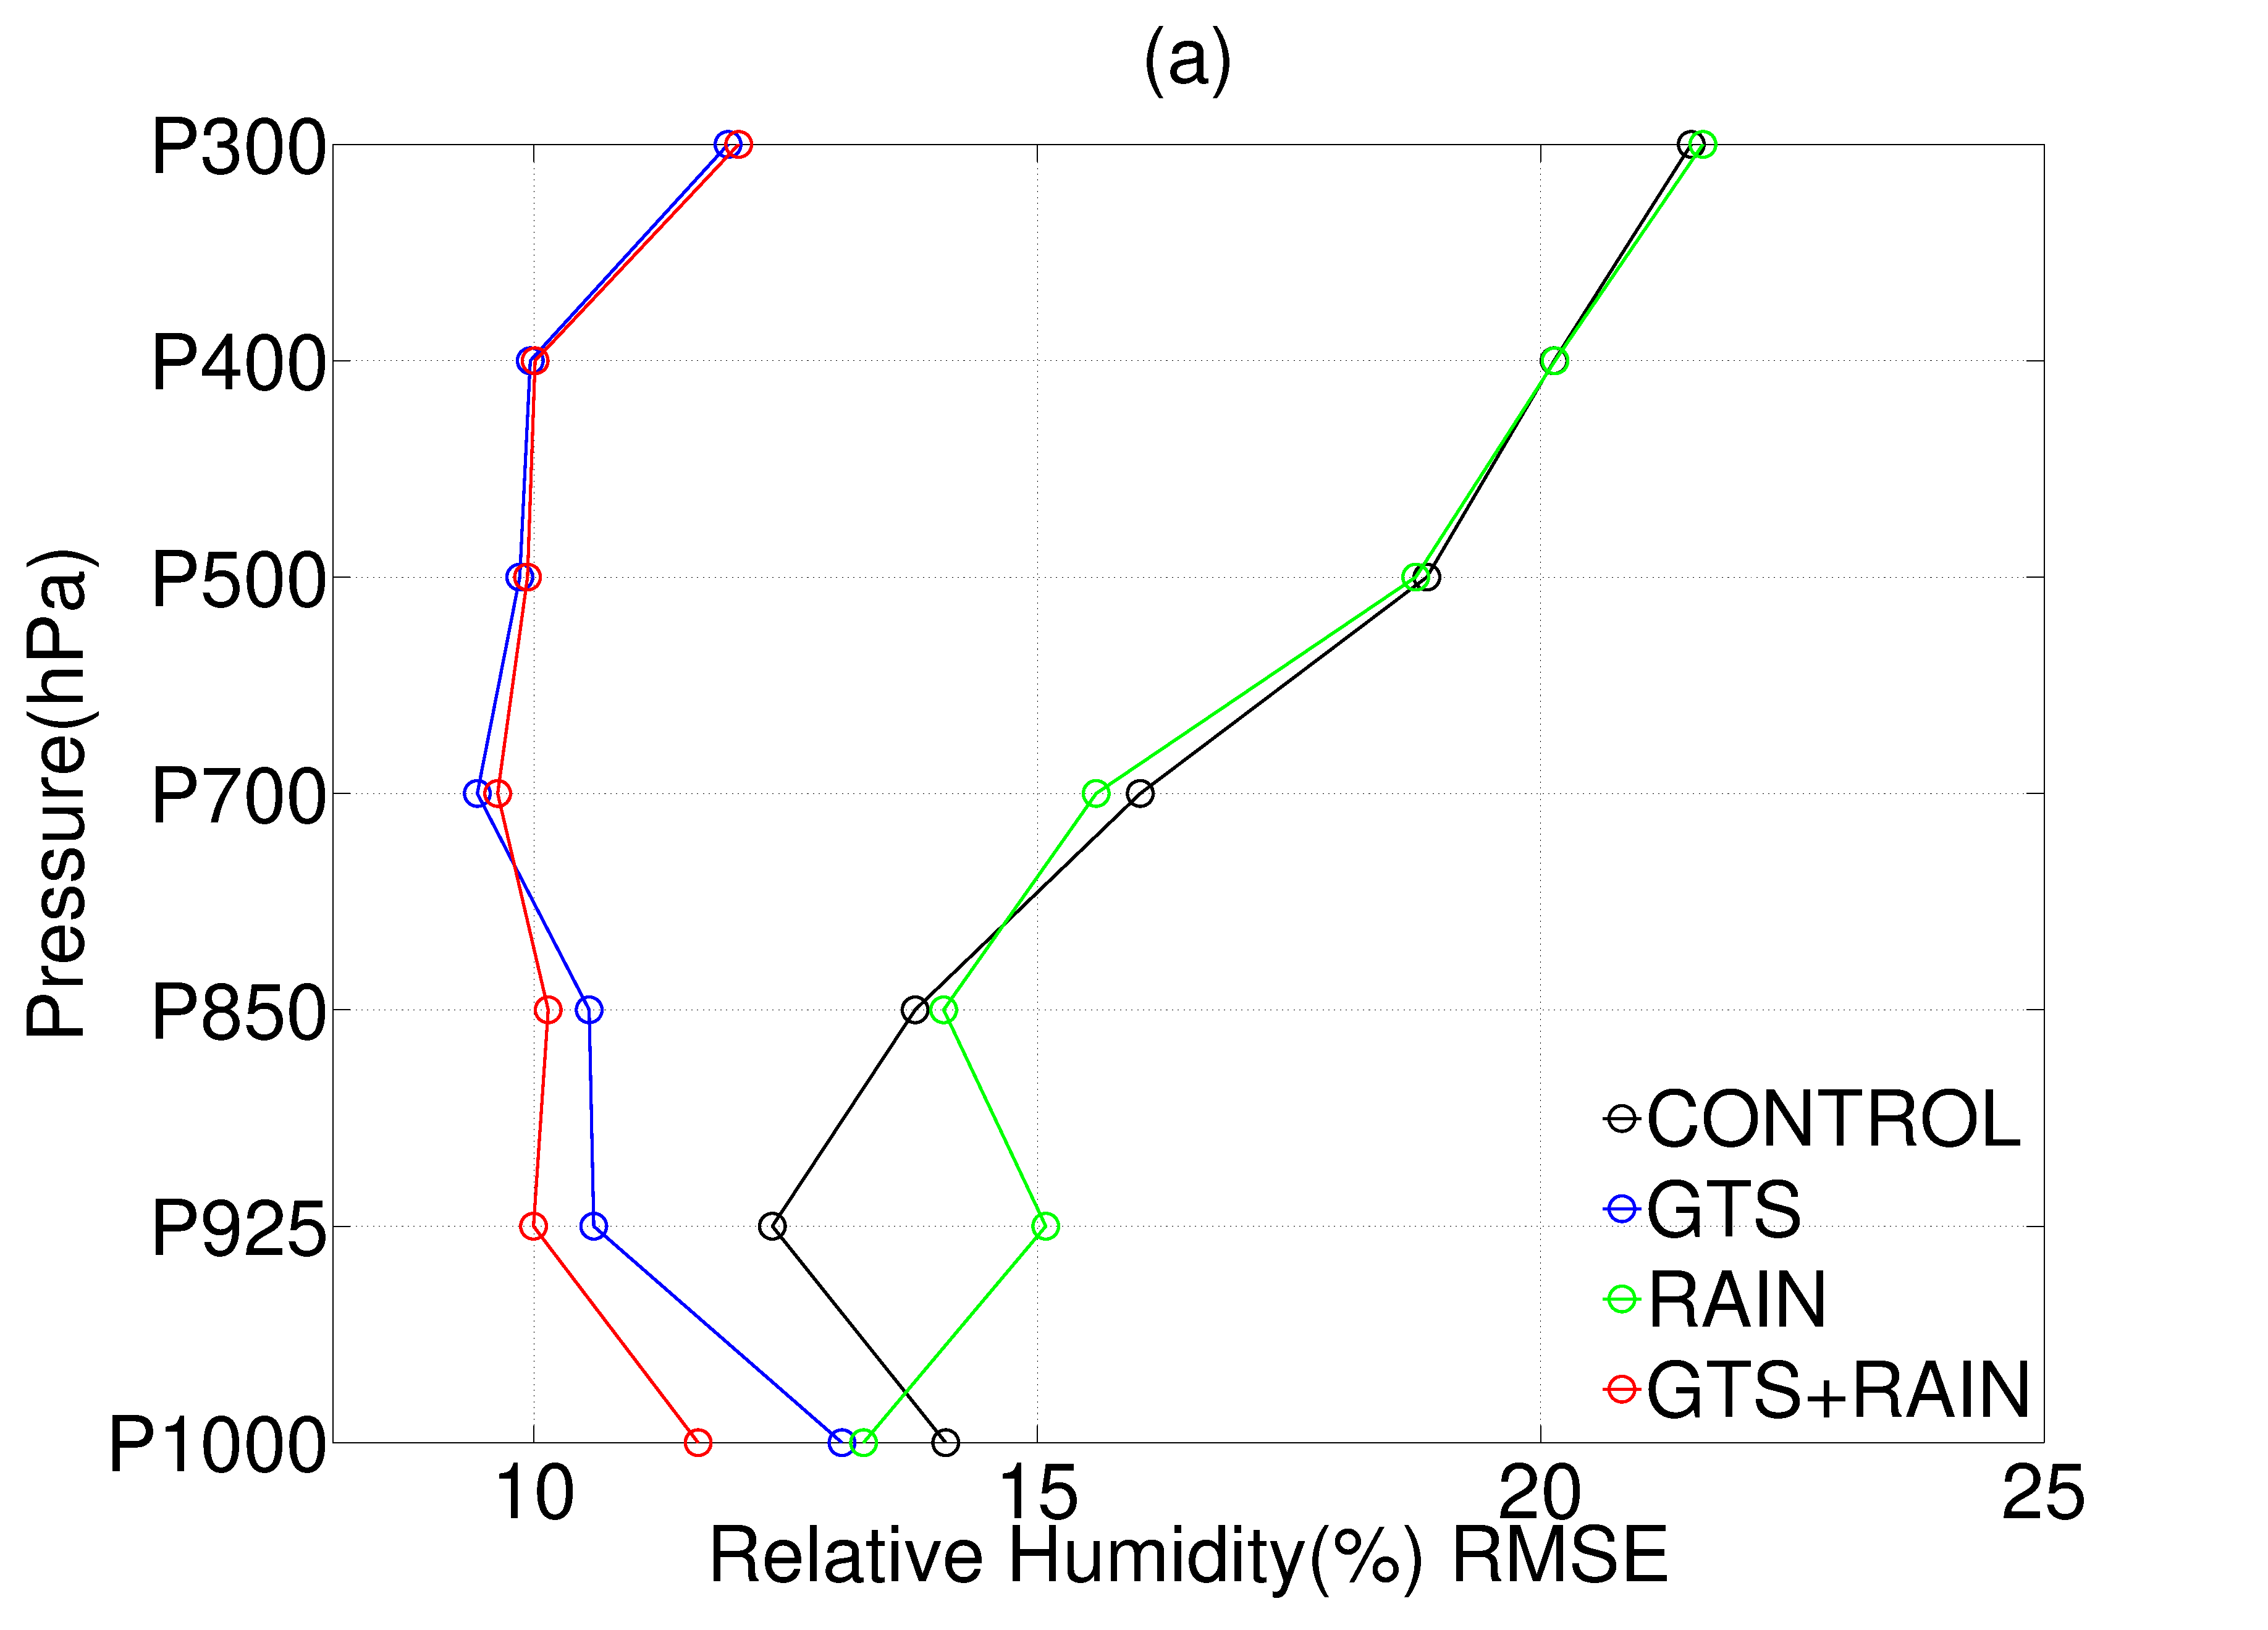
\includegraphics[width=0.5\linewidth]{./figures/rh_00.eps}

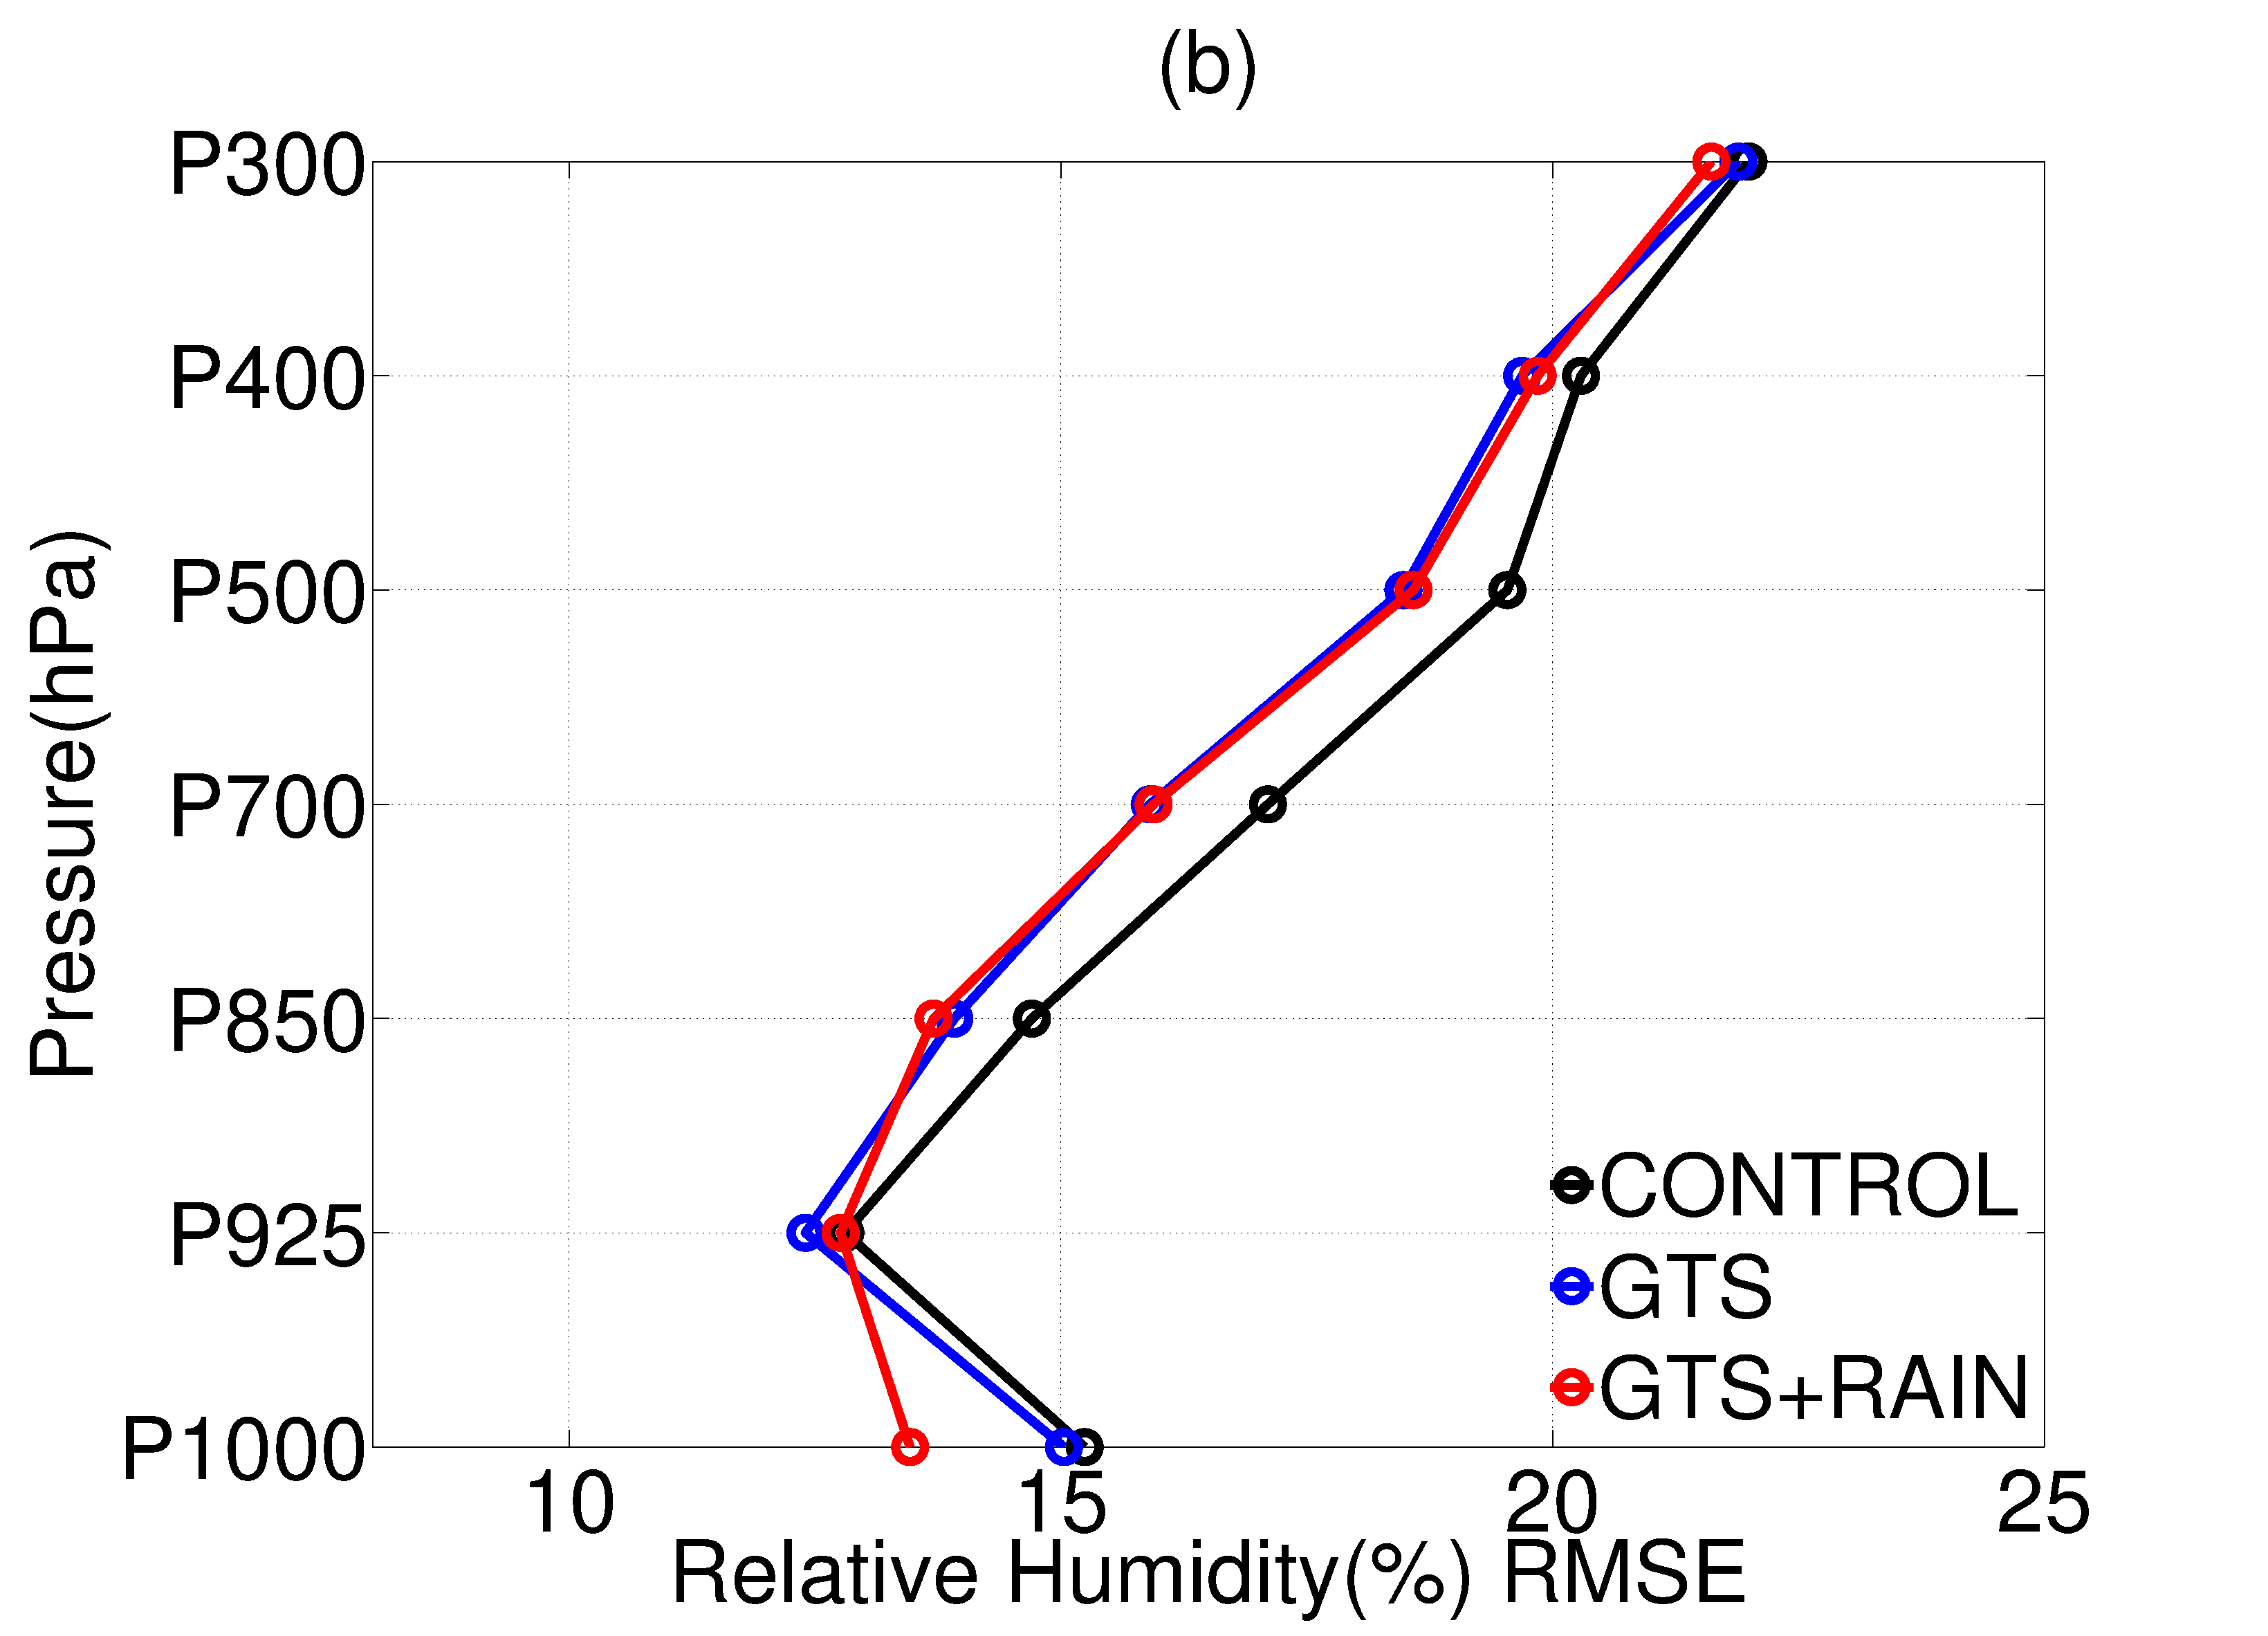
\includegraphics[width=0.5\linewidth]{./figures/rh_12.eps}

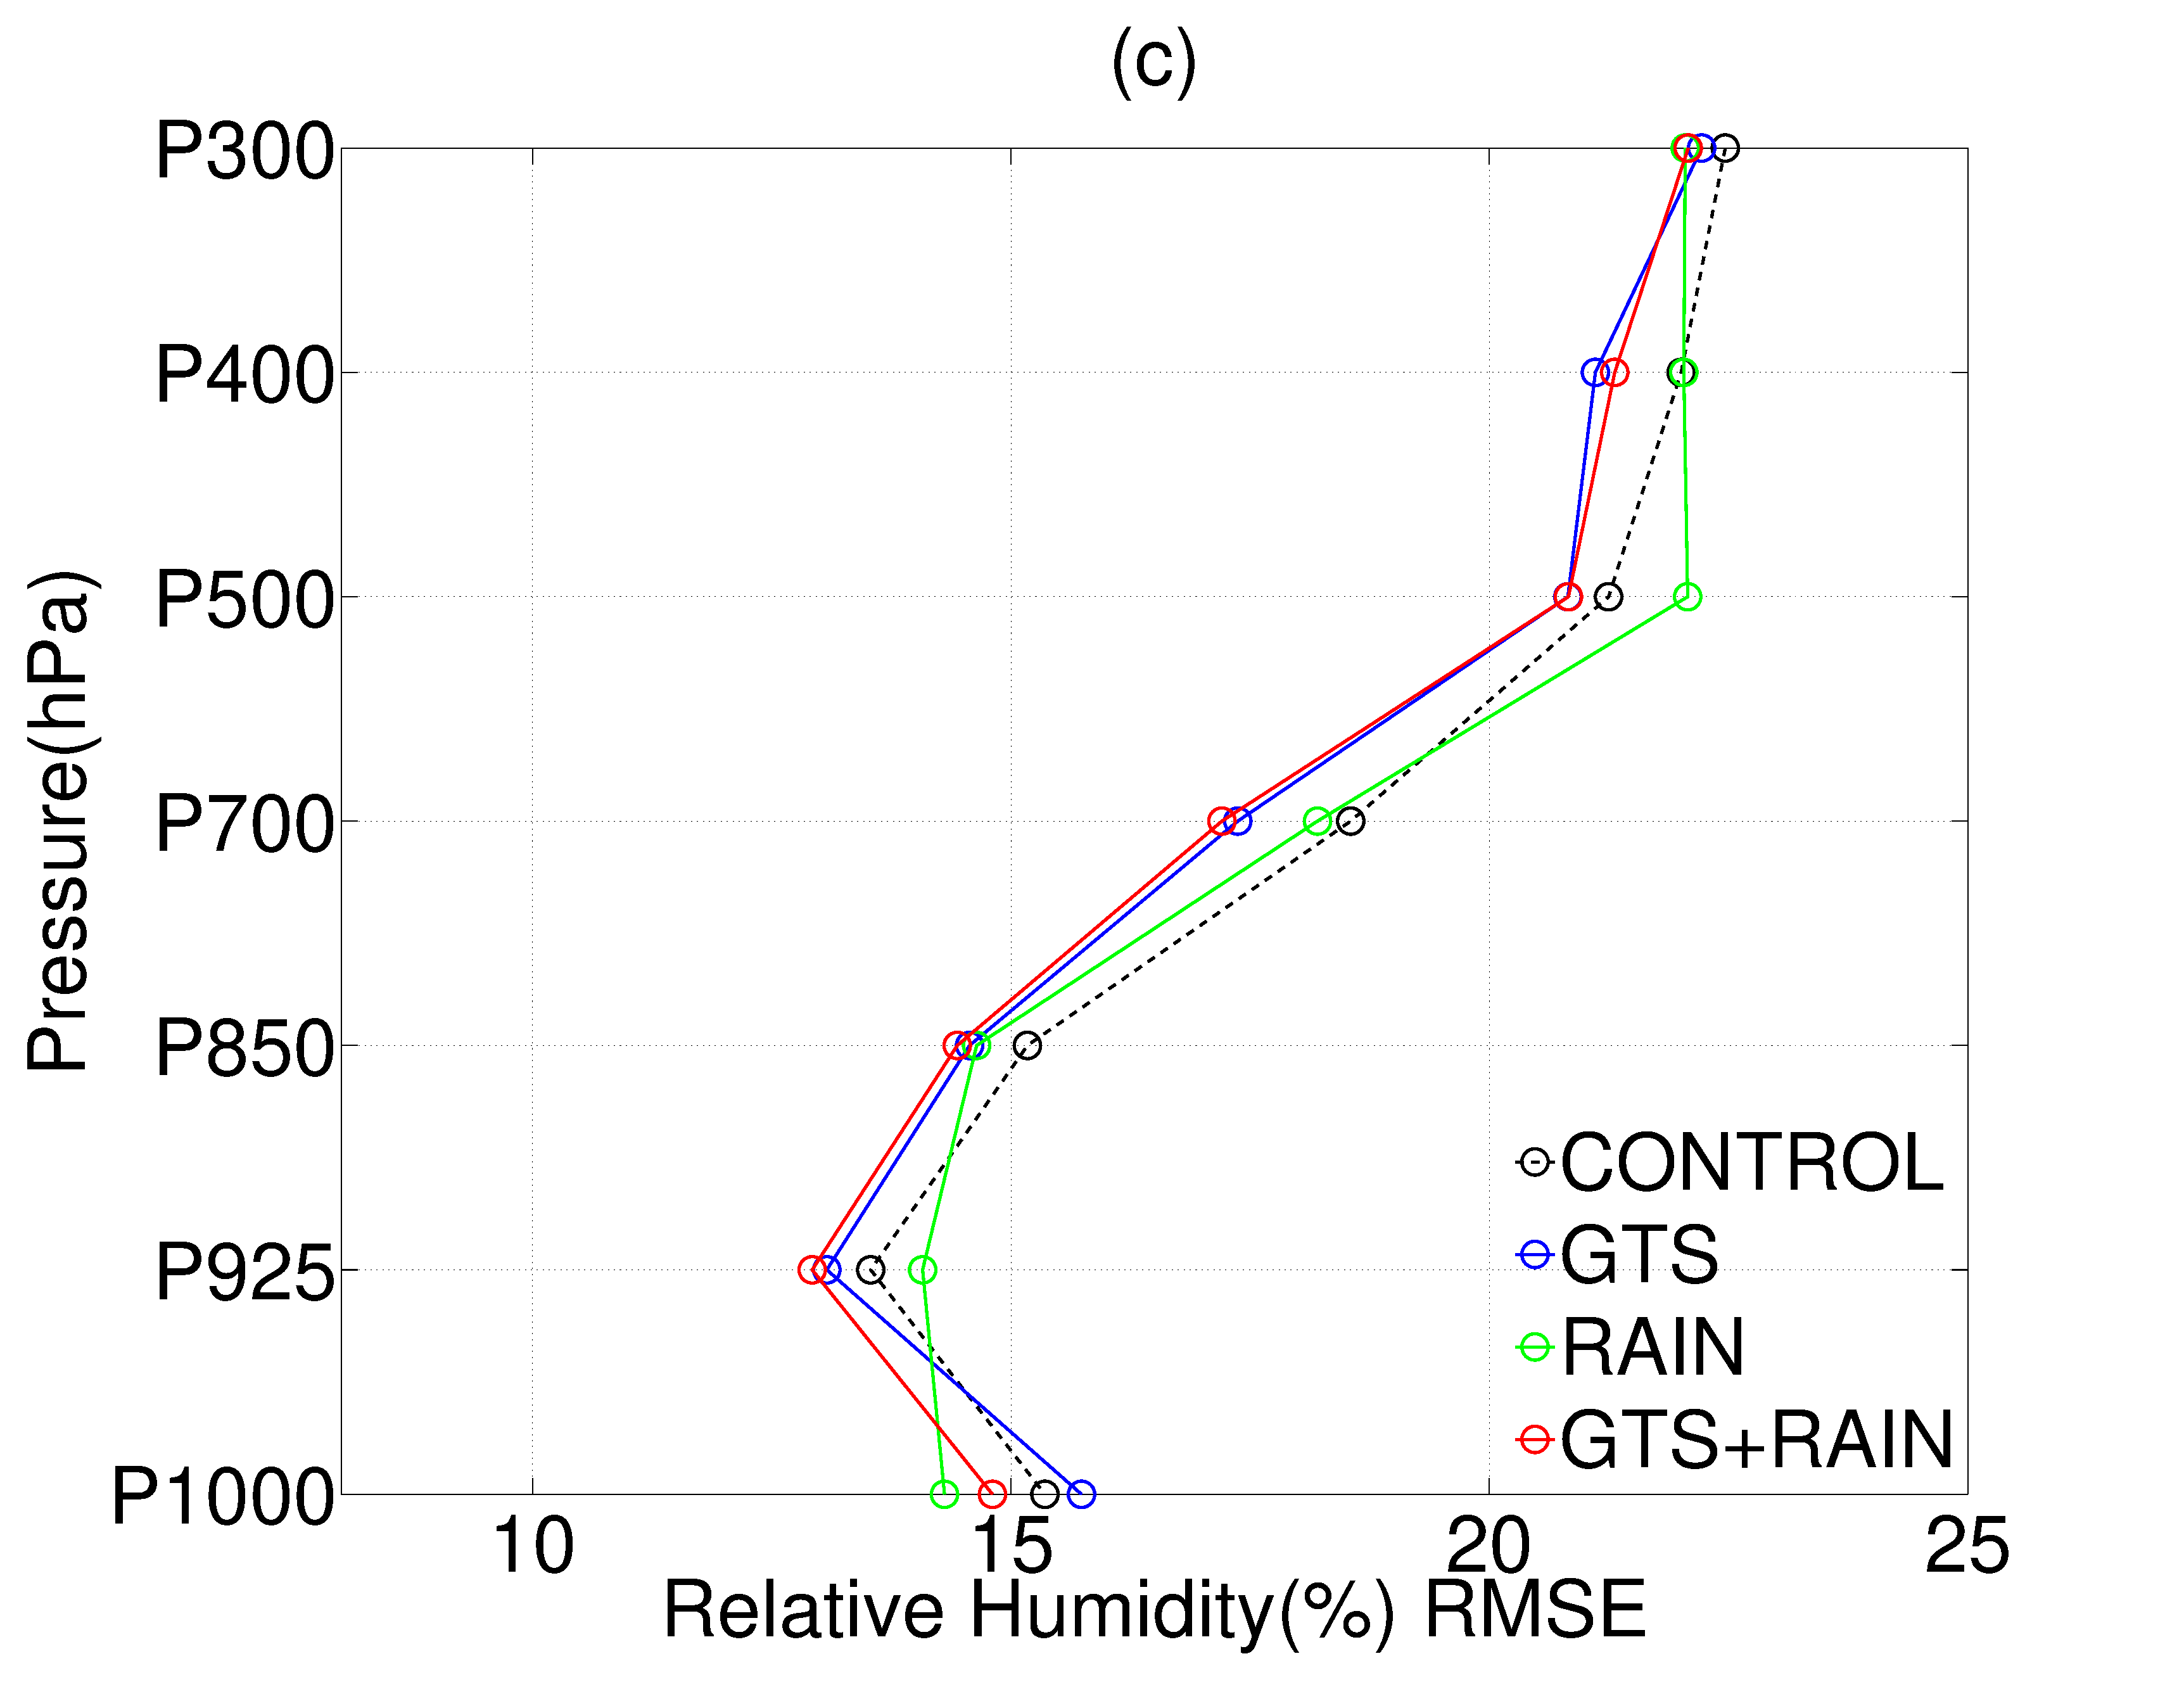
\includegraphics[width=0.5\linewidth]{./figures/rh_24.eps}
\caption{Same as Figure 1 but for relative humidity.}\label{rh_00}
\end{figure}

\newpage
\begin{figure}
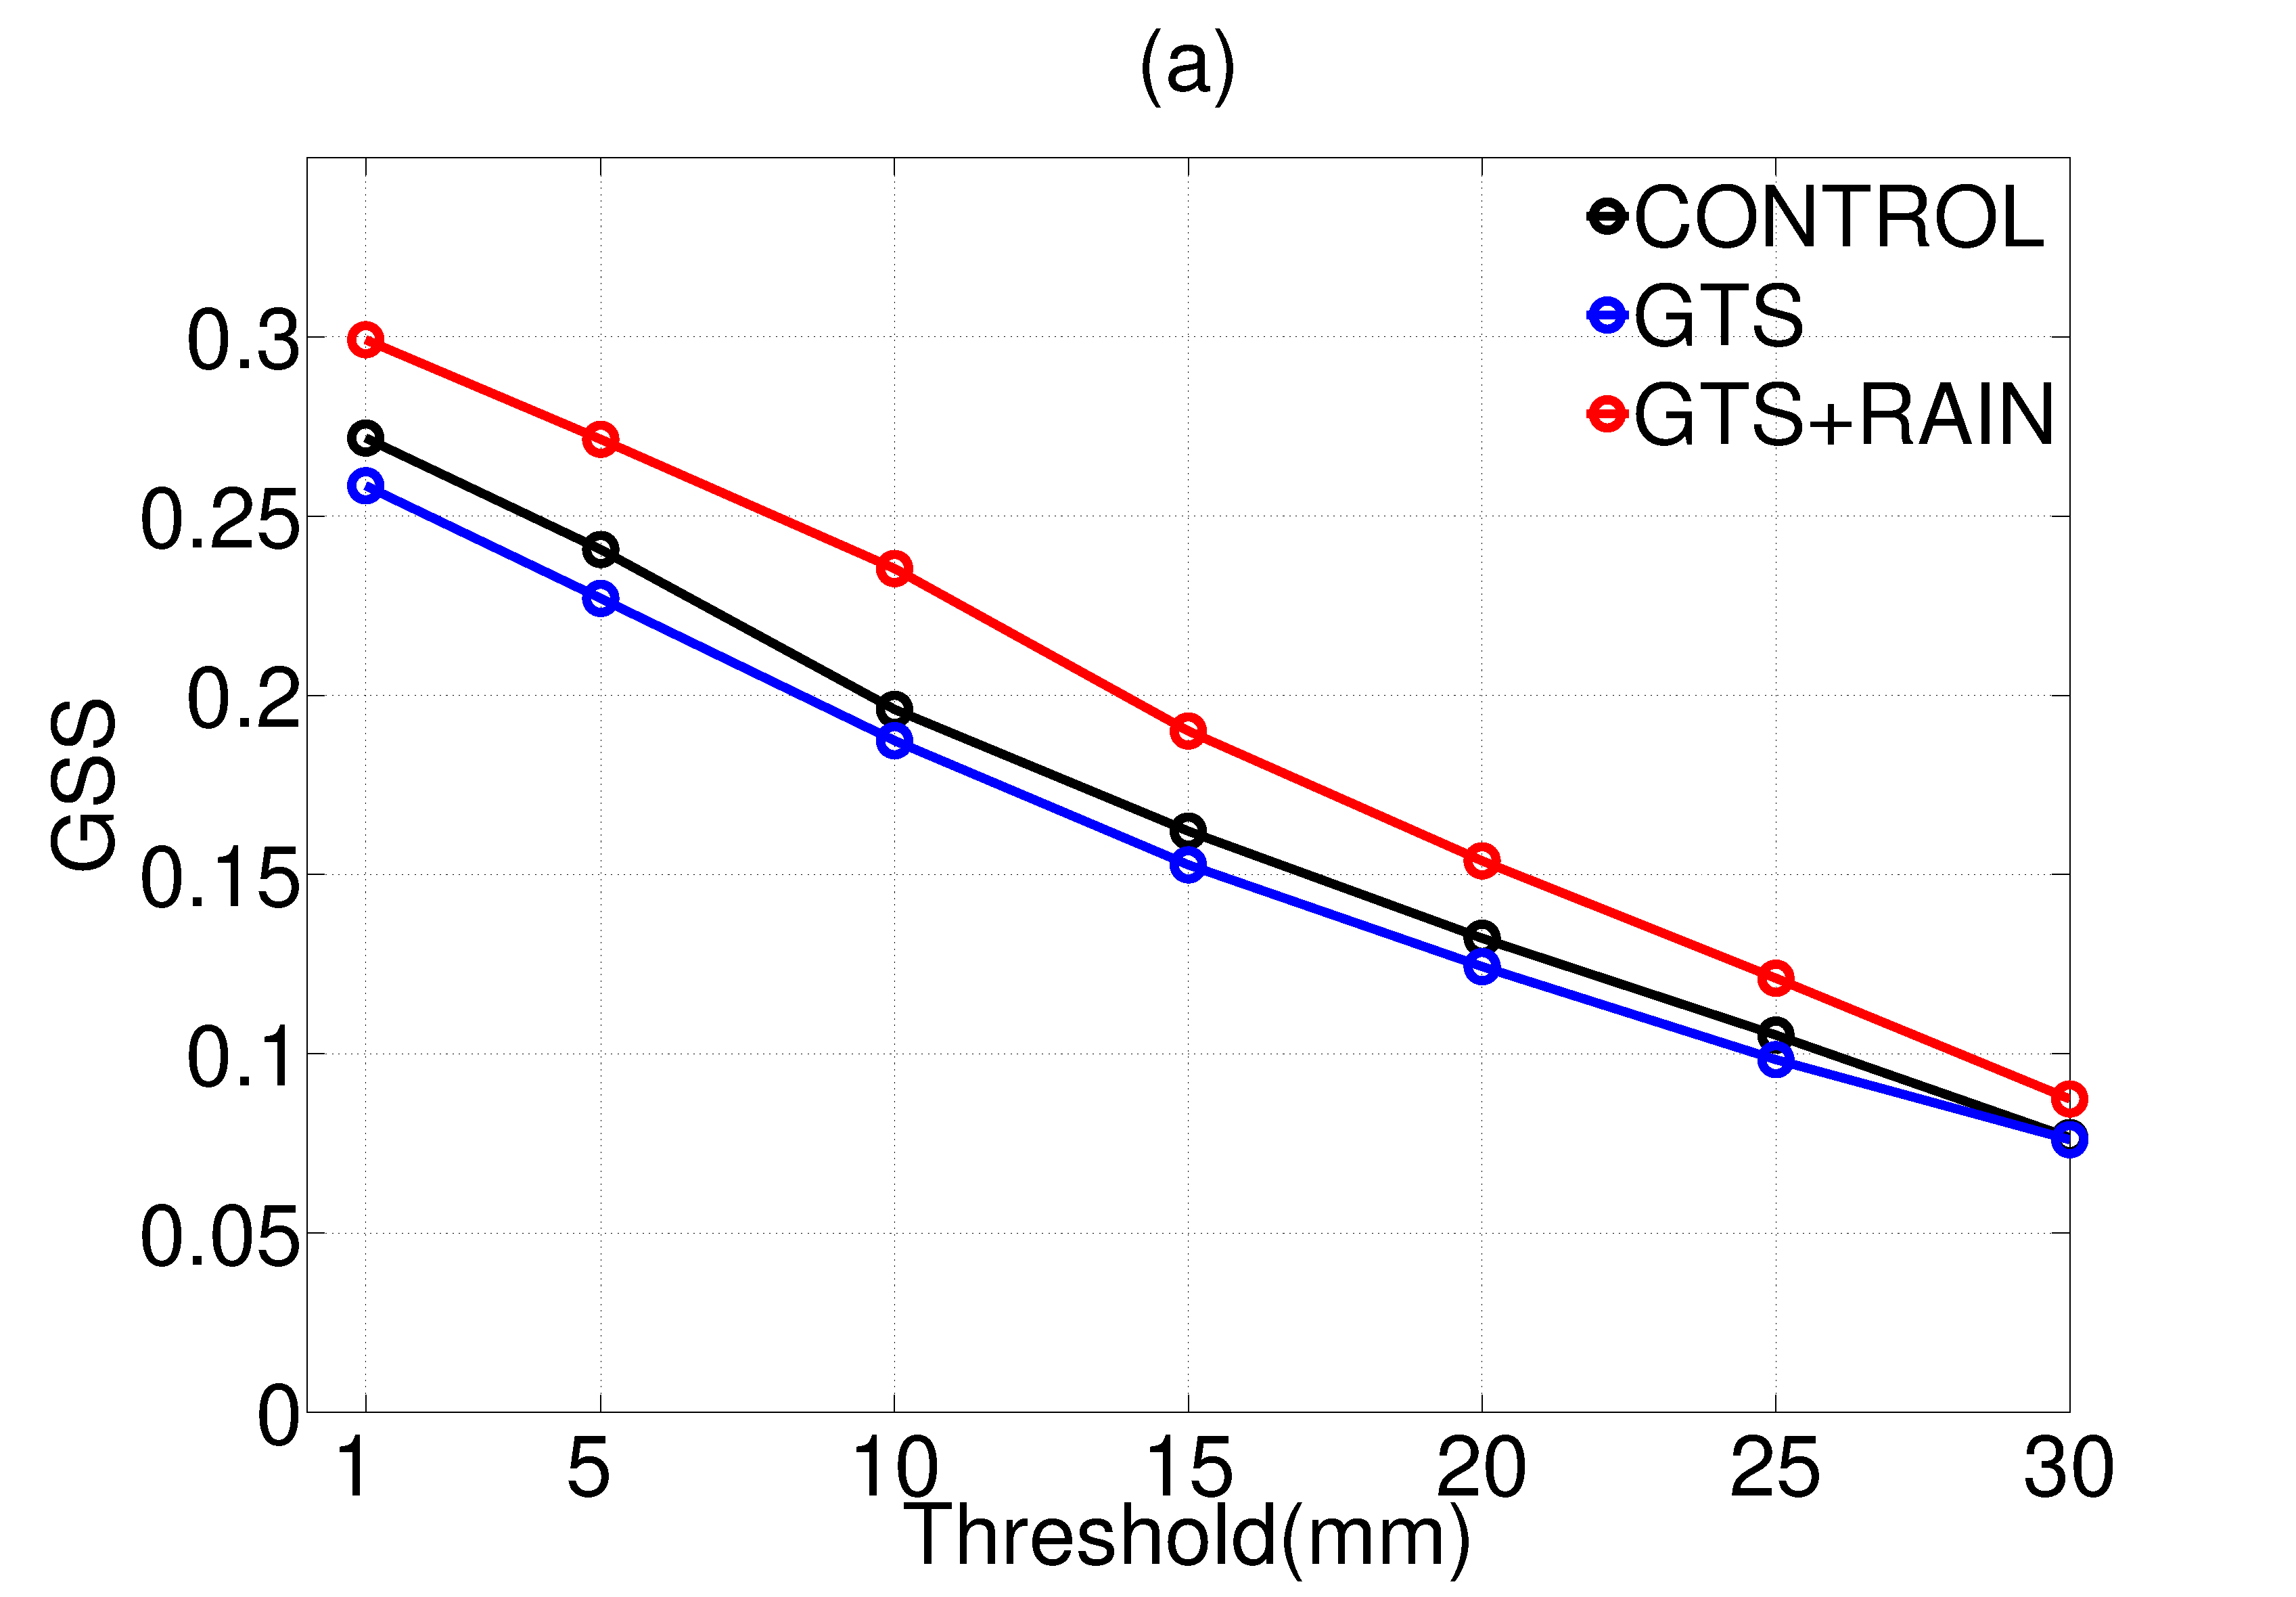
\includegraphics[width=0.5\linewidth]{./figures/GSS_12.eps}
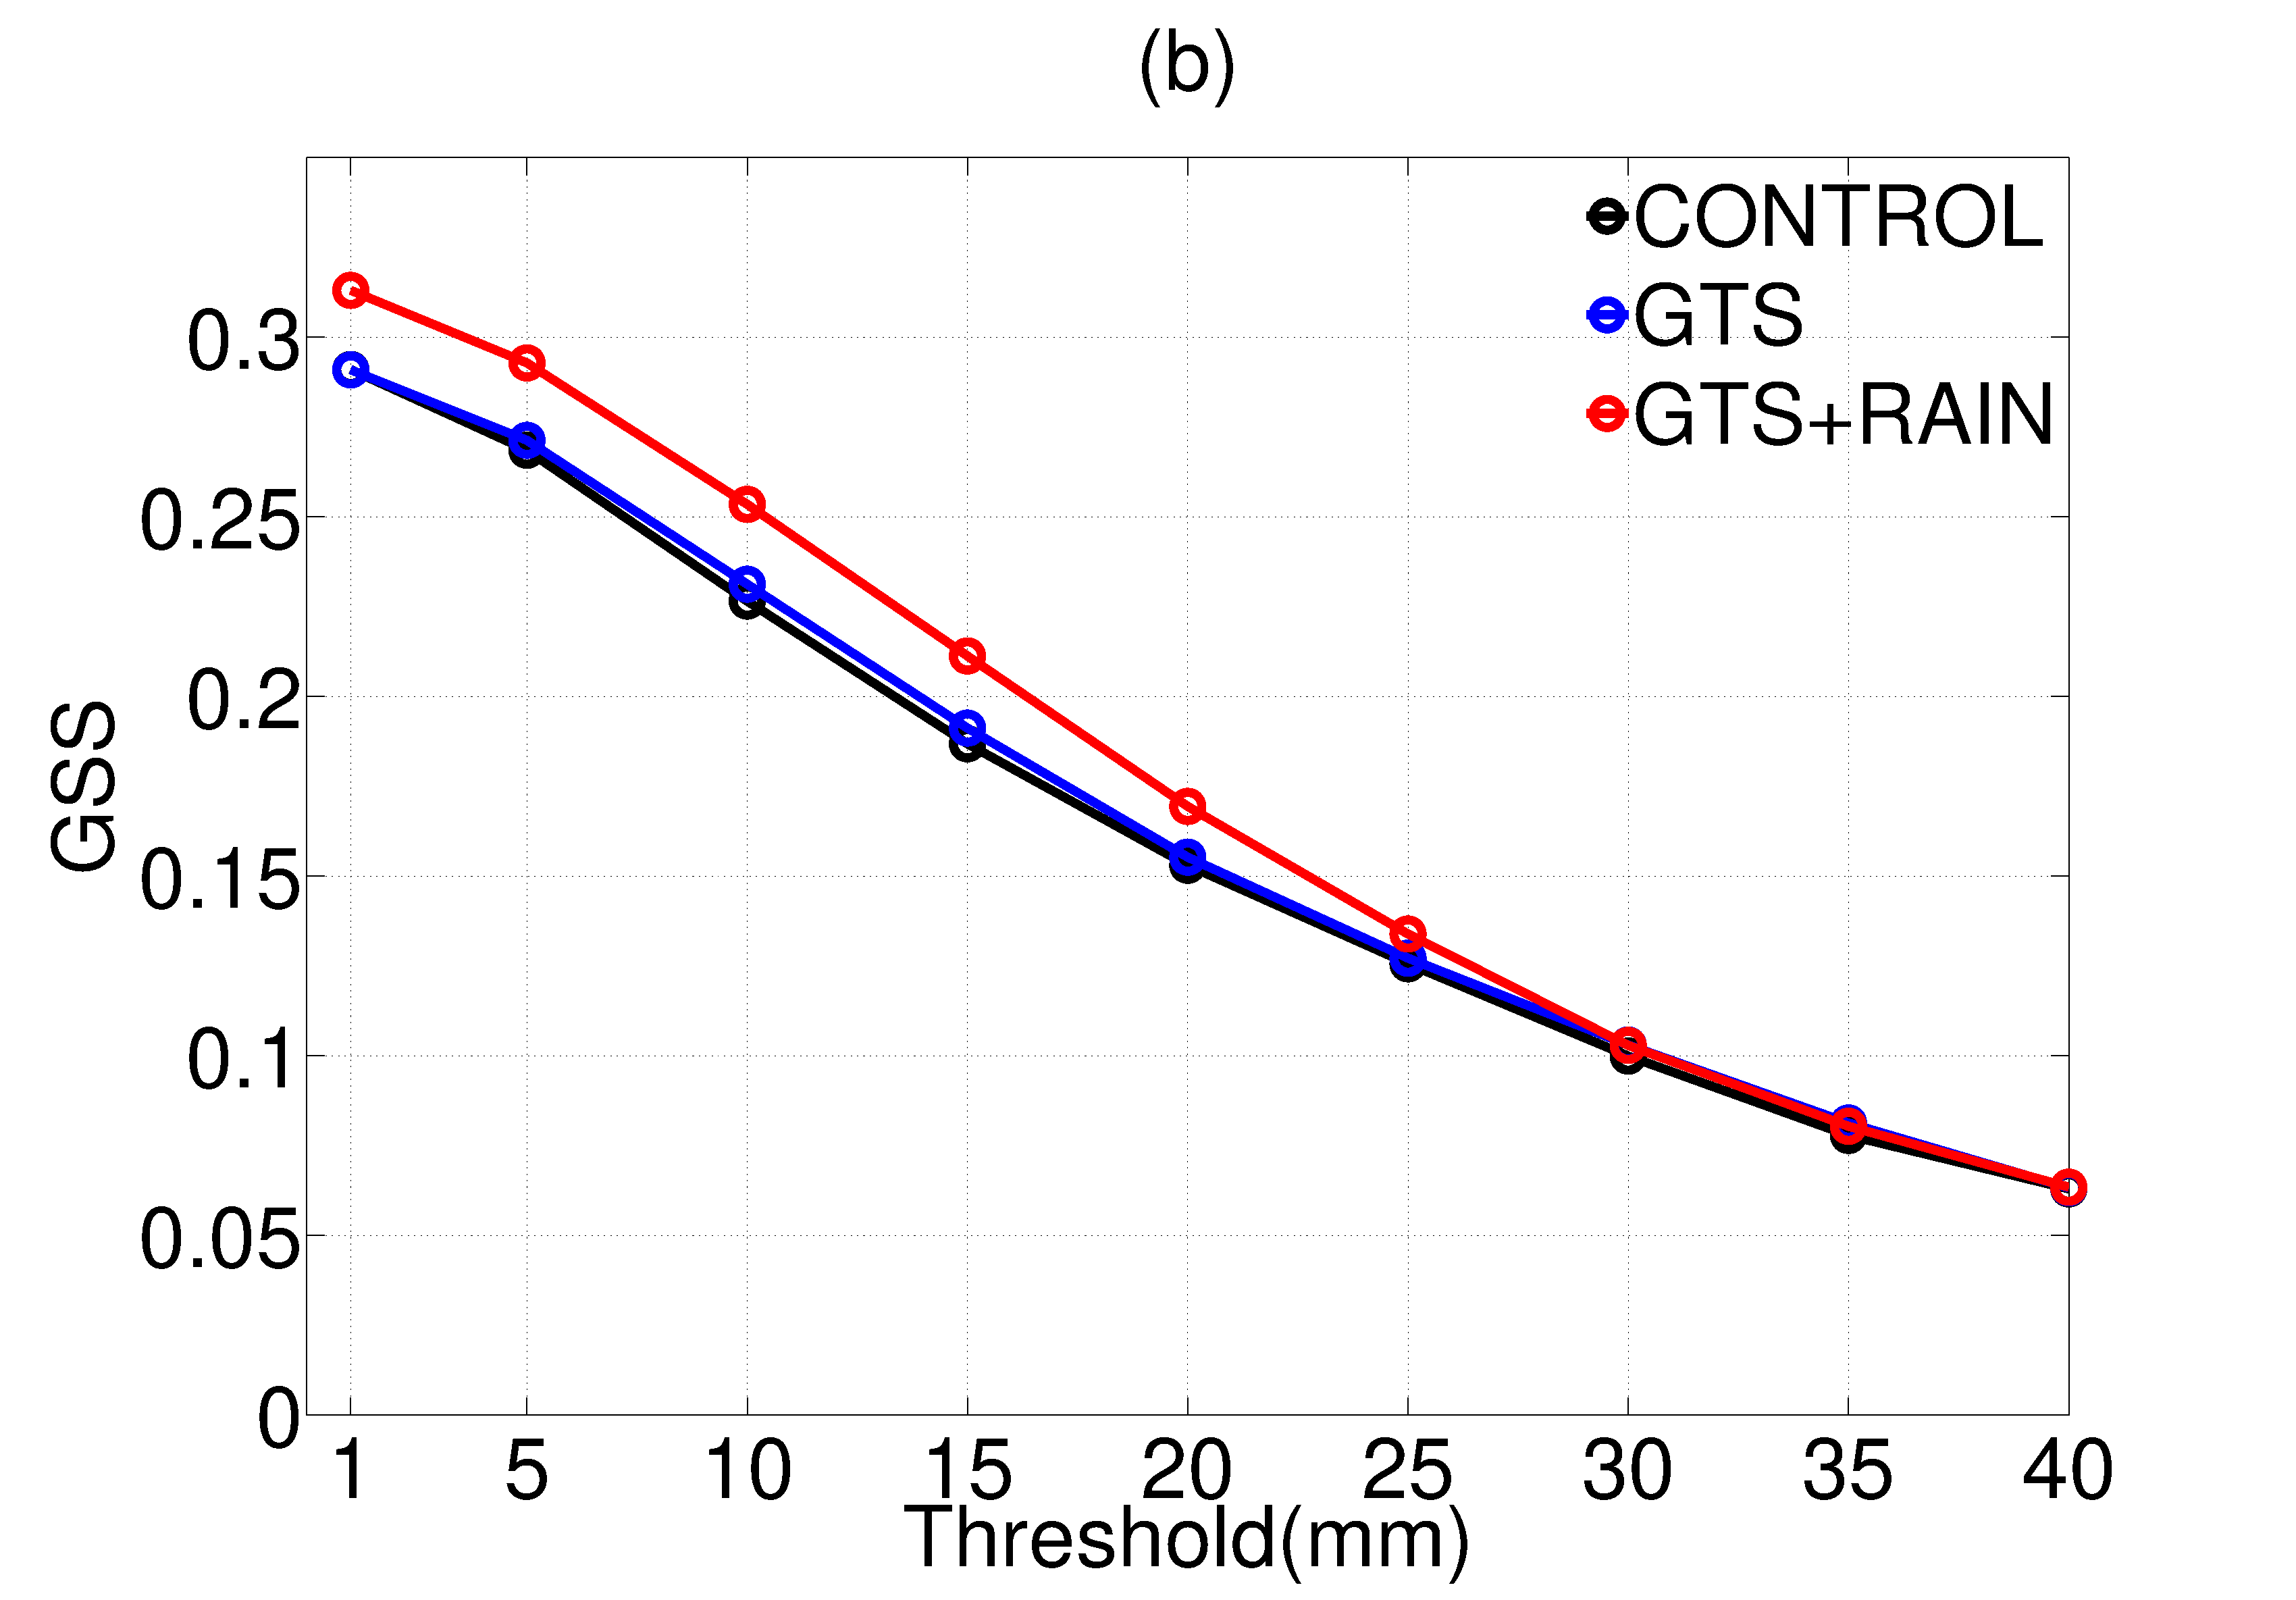
\includegraphics[width=0.5\linewidth]{./figures/GSS_24.eps}
\caption{Threshold series of GSS for 12-h (a) and 24-h (b) accumulated precipitation from the experiment CONTROL, GTS, GTS+RAIN. }\label{gss_12h}
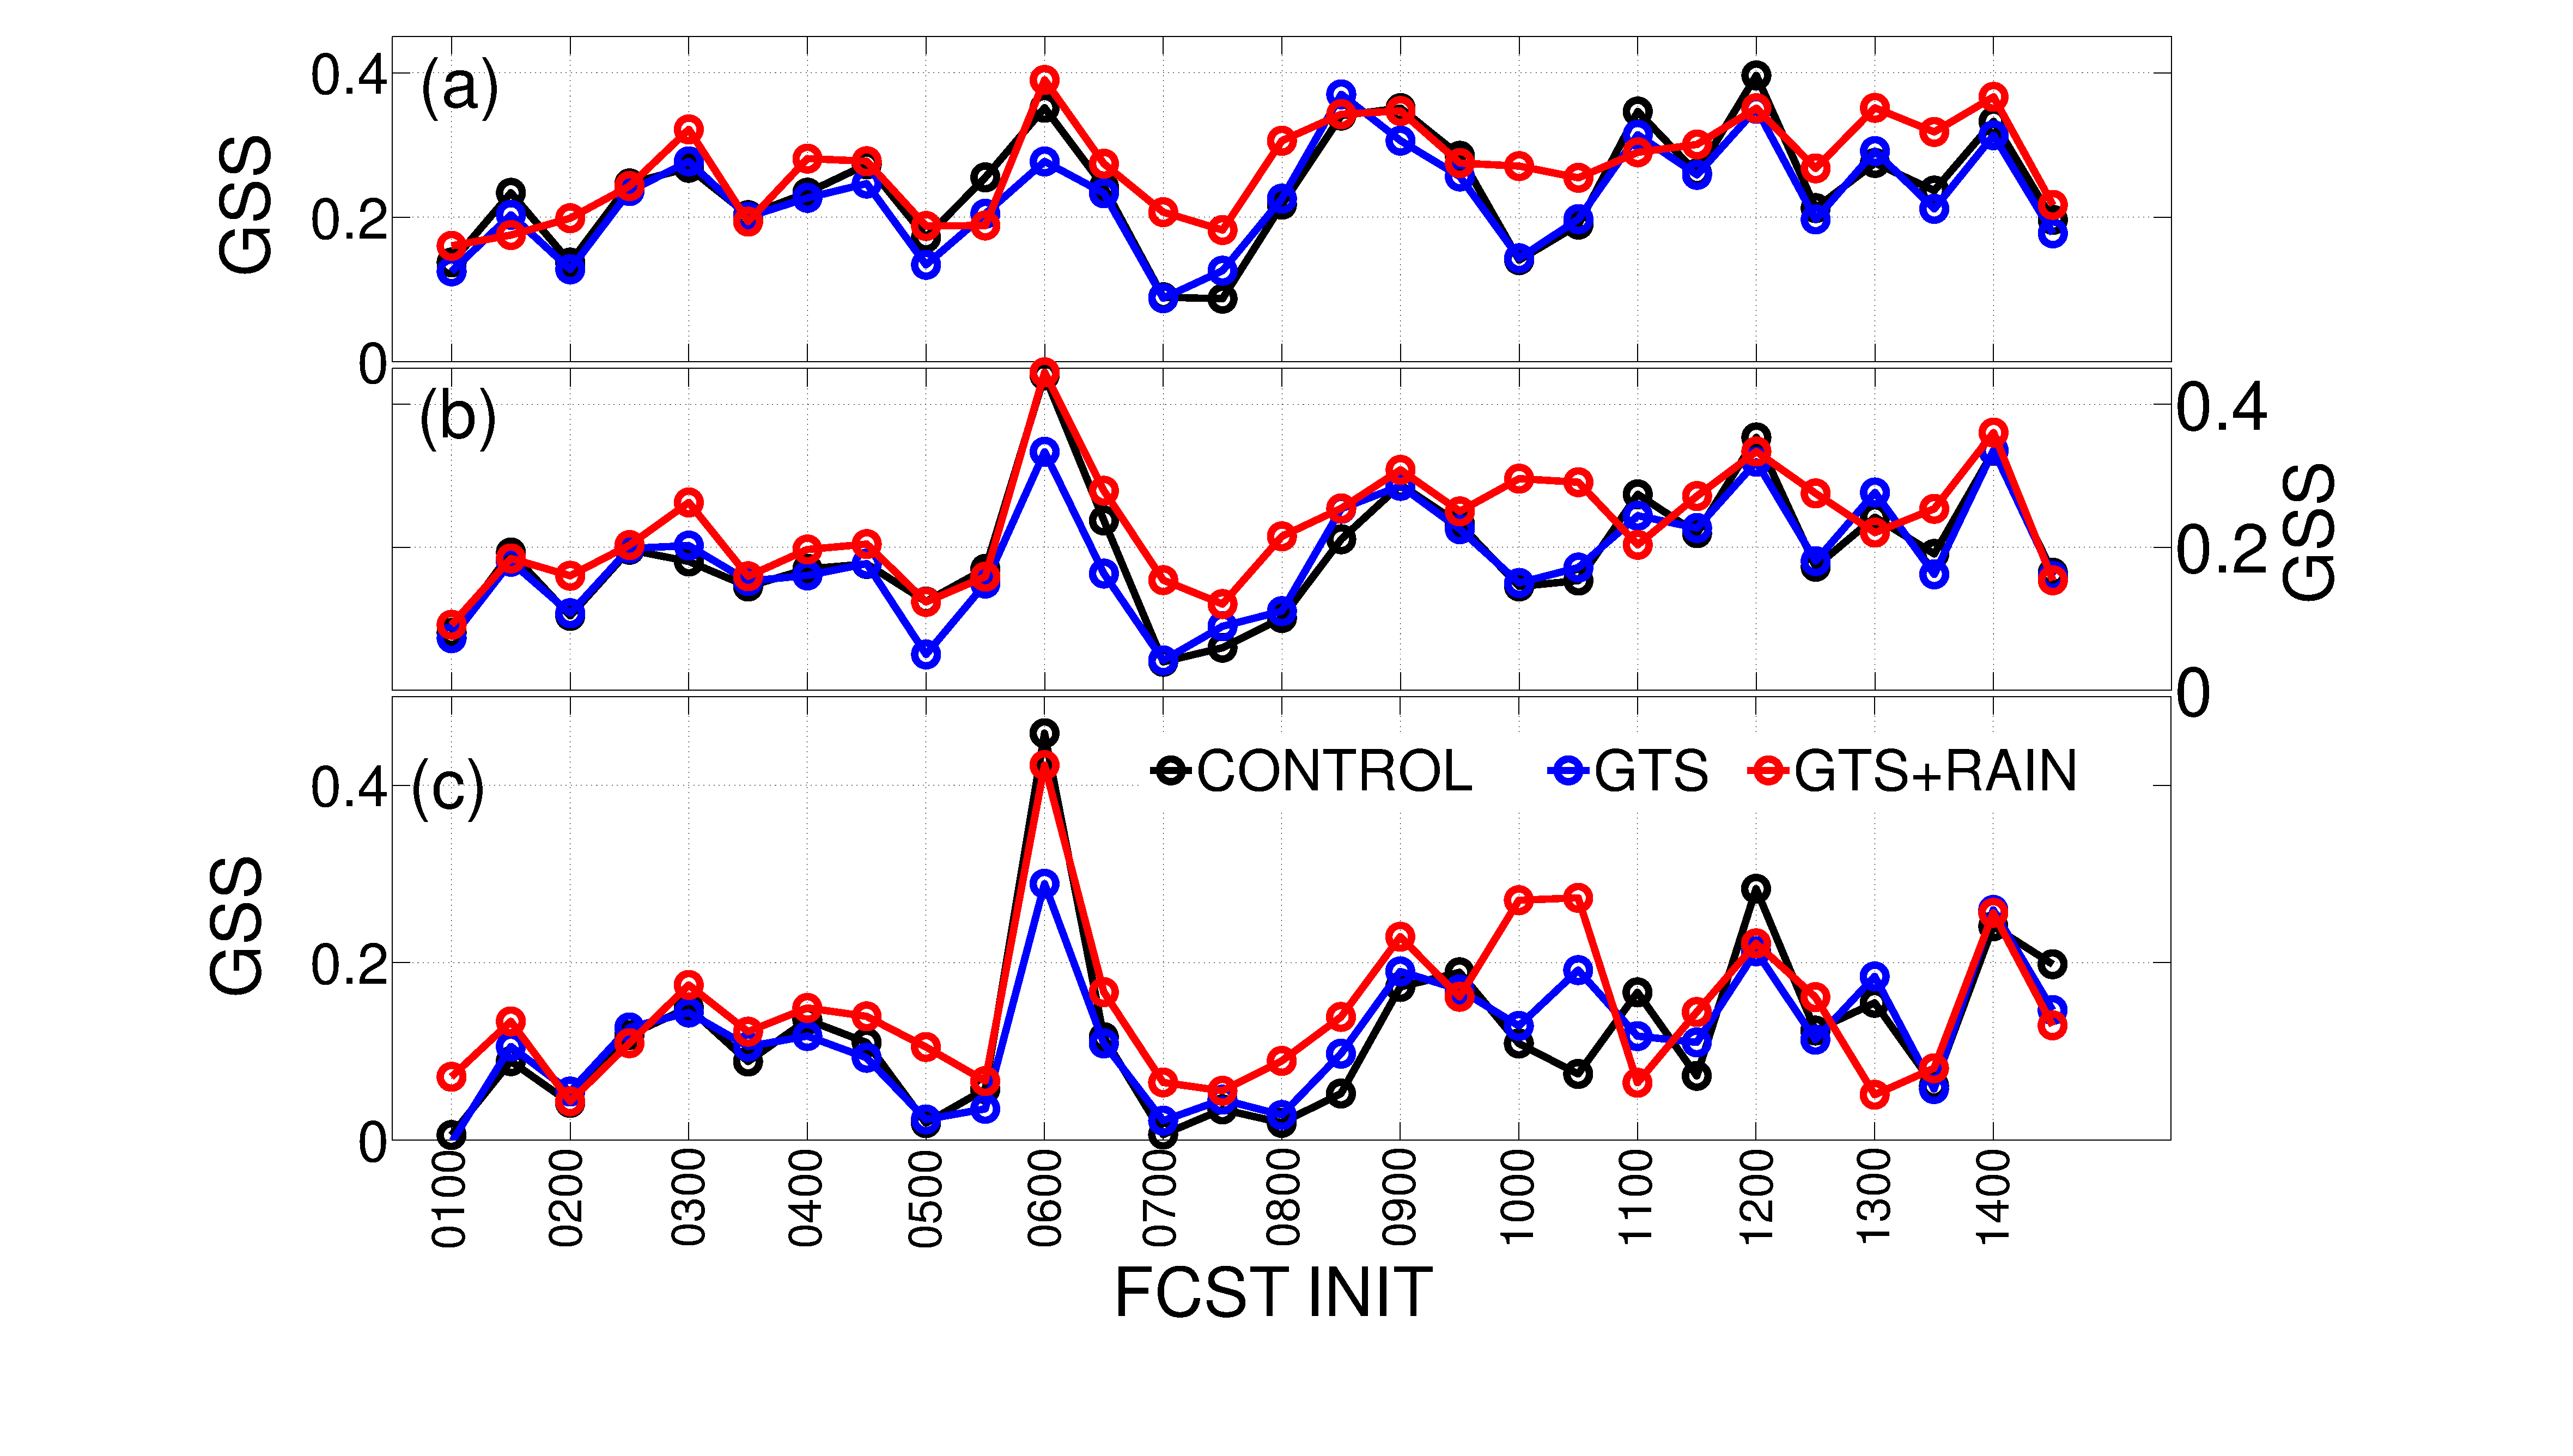
\includegraphics[width=0.8\linewidth]{./figures/GSS_timeser.eps}
\caption{Time series of Gilberty Skill Score (GSS) from 0000 UTC 1 to 1200 UTC 14 June 2010. The 12-h accumulated precipitation from the experiment CONTROL, GTS, GTS+RAIN are verified against NCEP Stage IV gridded precipitation at different thresholds (a) 5.0mm, (b) 10.0 mm and (c) 20.0 mm. }\label{timeser}
\end{figure}

\newpage
\begin{figure}
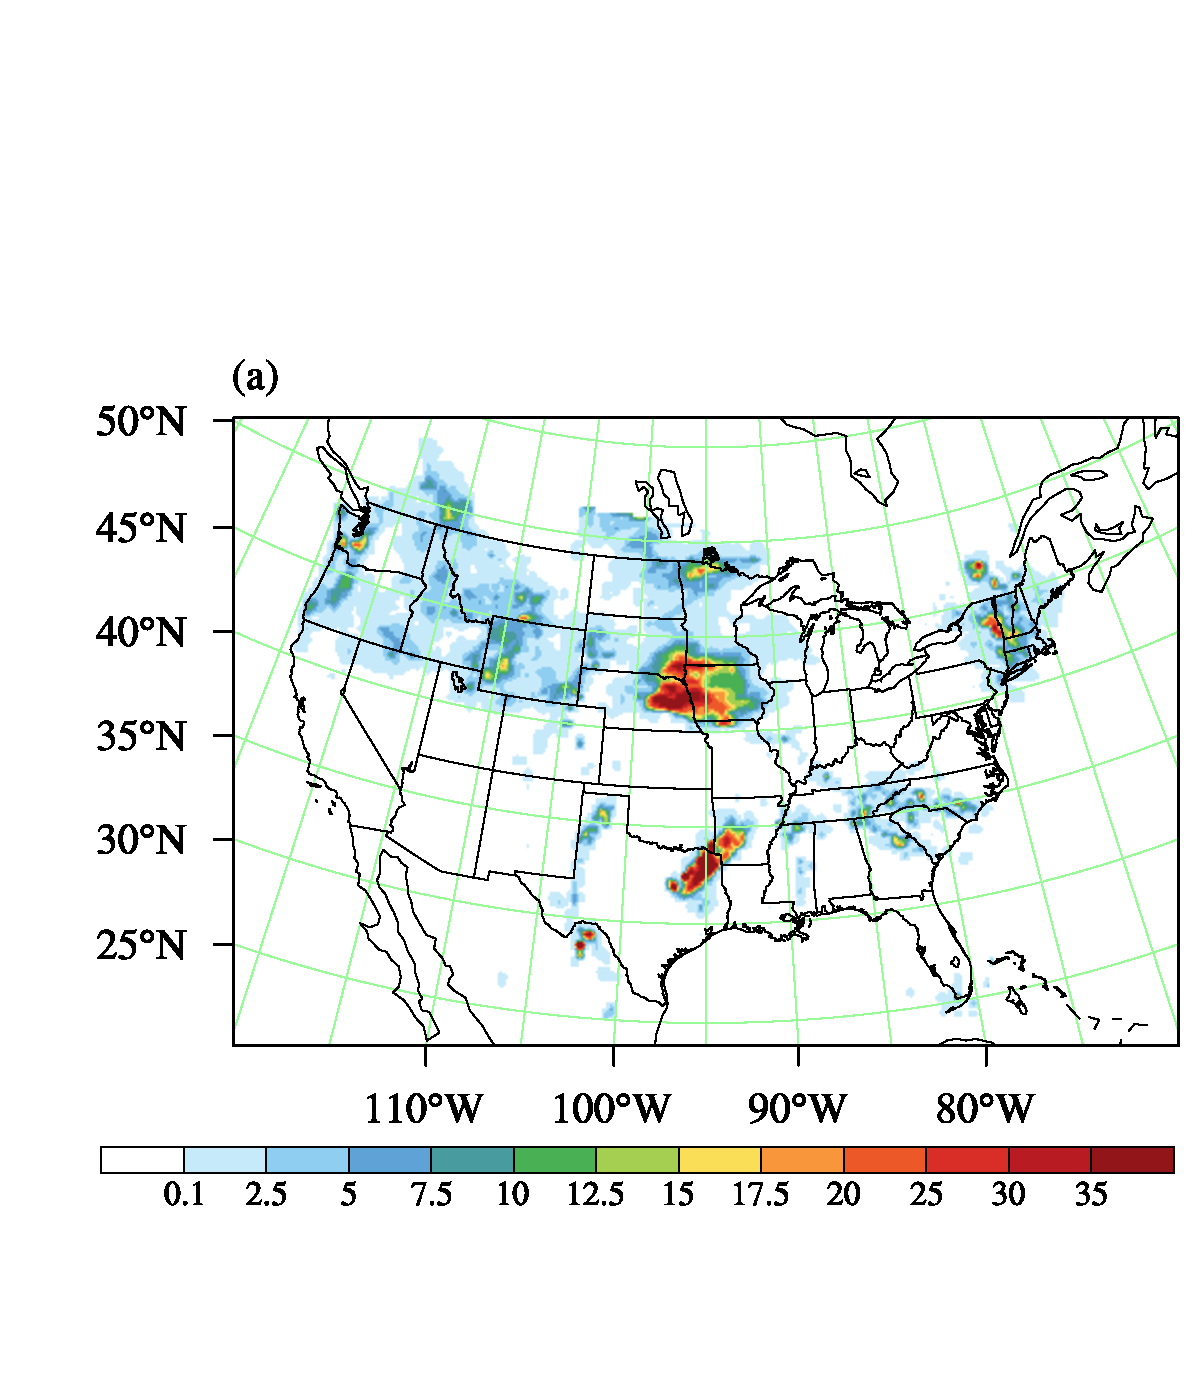
\includegraphics[width=0.4\linewidth]{./figures/st4_copy.pdf}

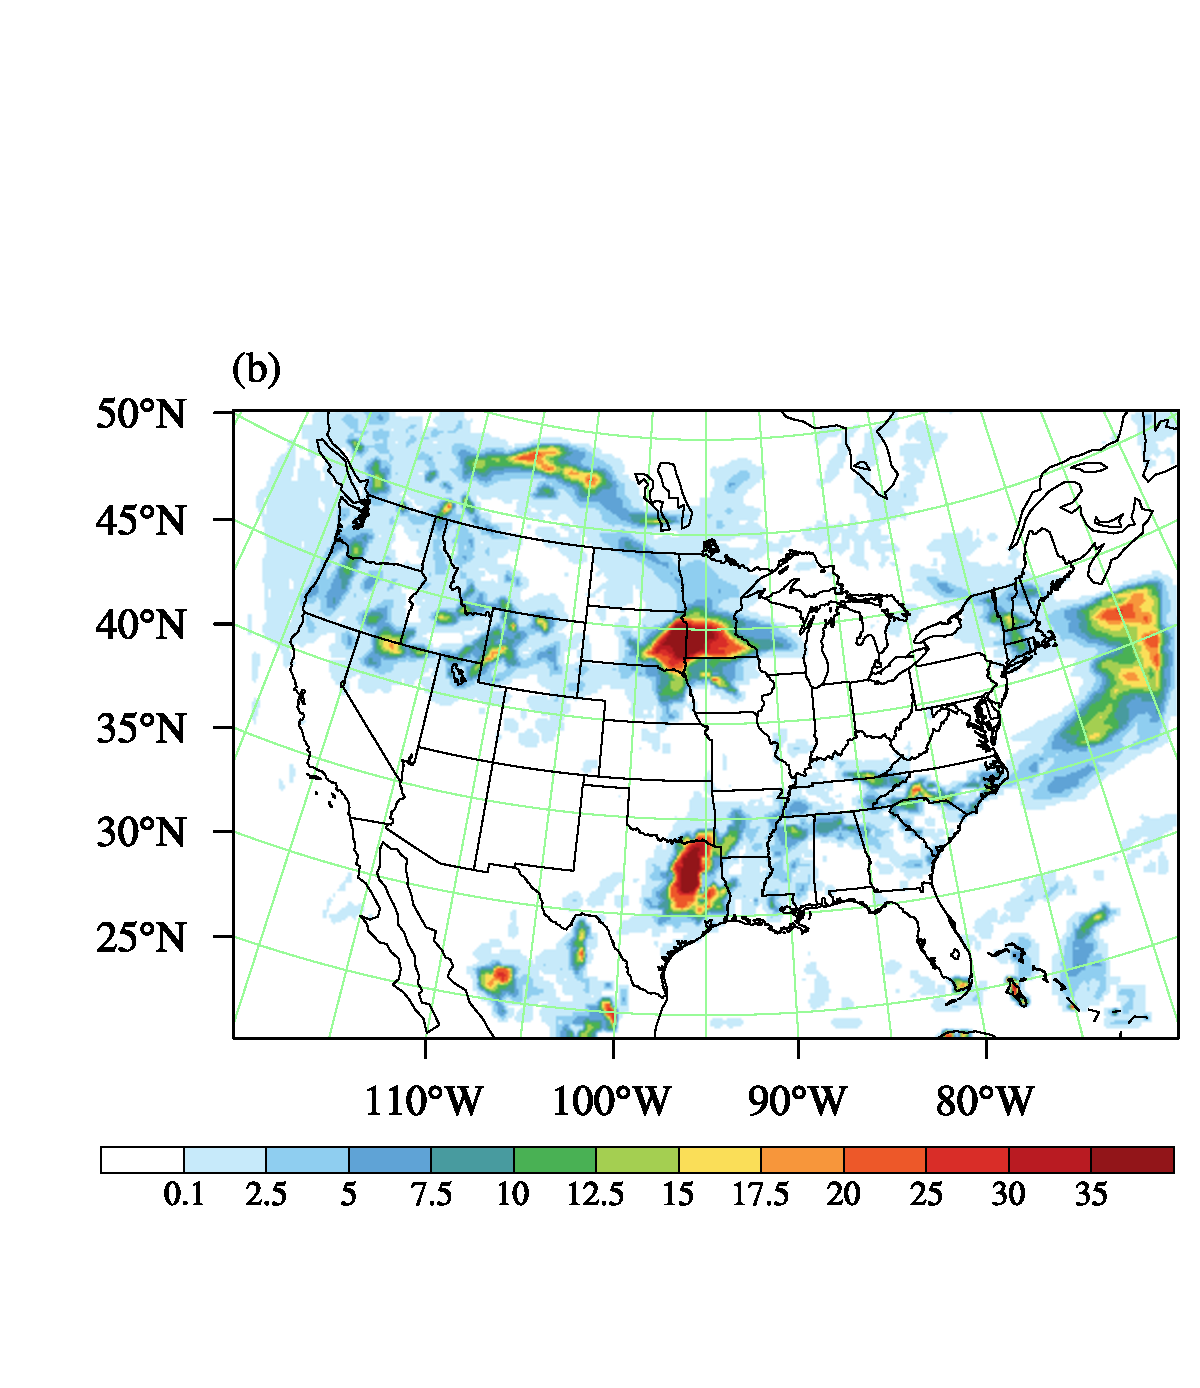
\includegraphics[width=0.4\linewidth]{./figures/control_copy.pdf}

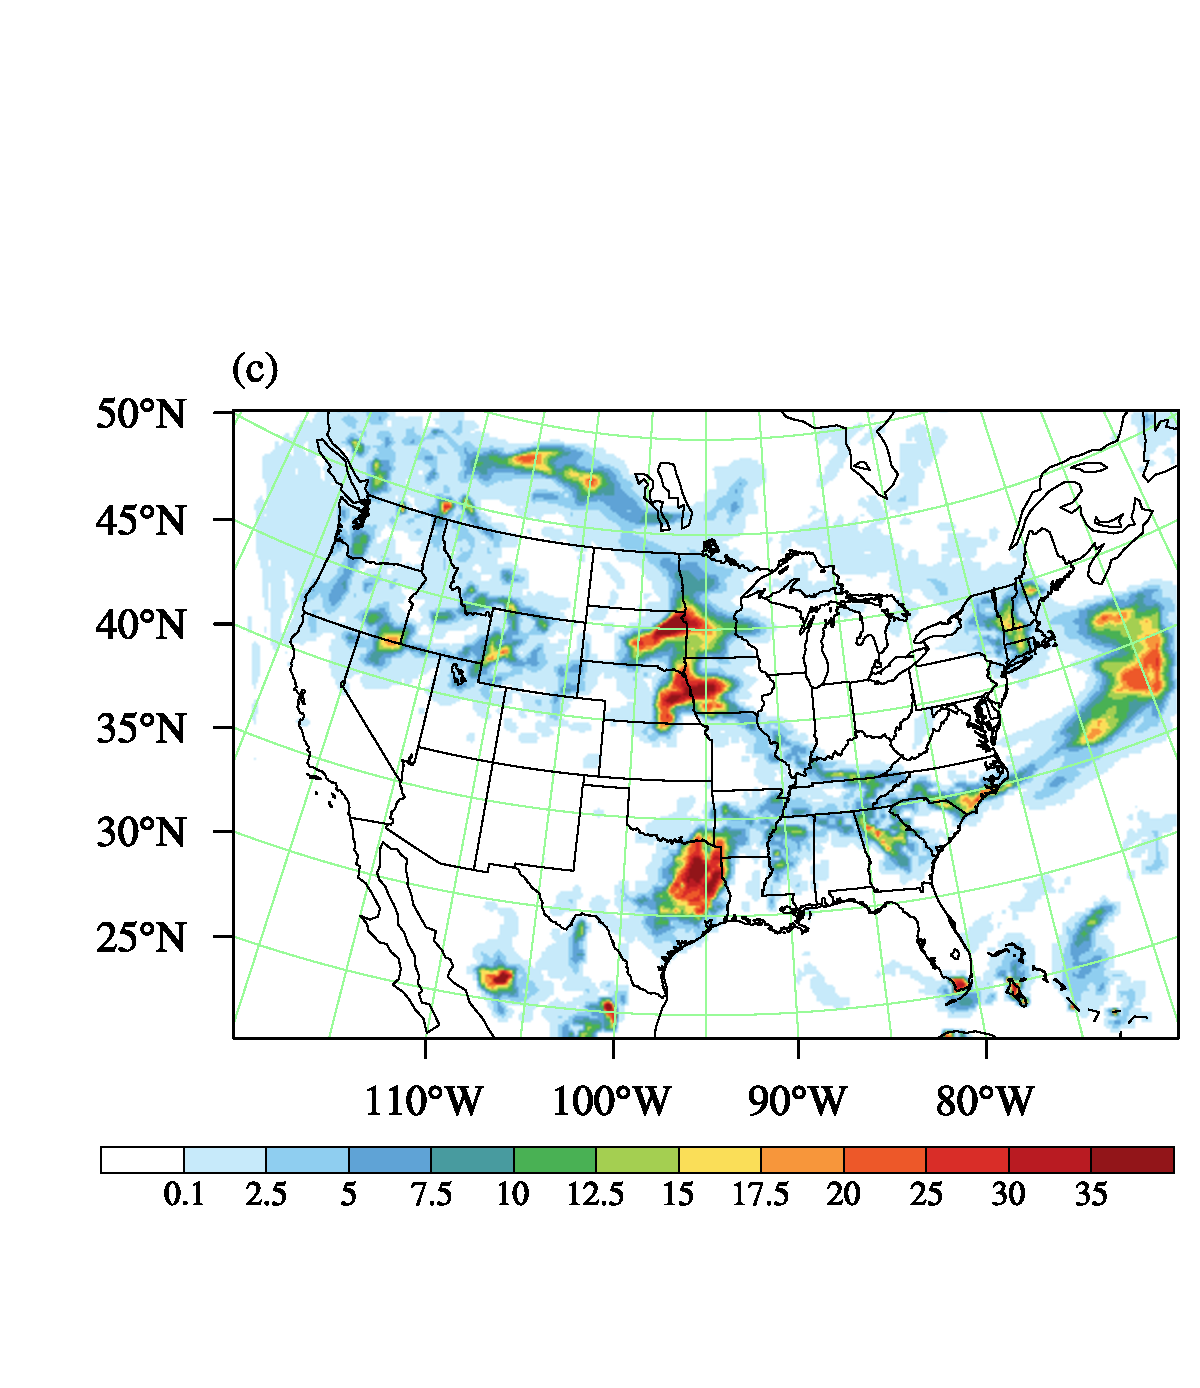
\includegraphics[width=0.4\linewidth]{./figures/gts_copy.pdf}

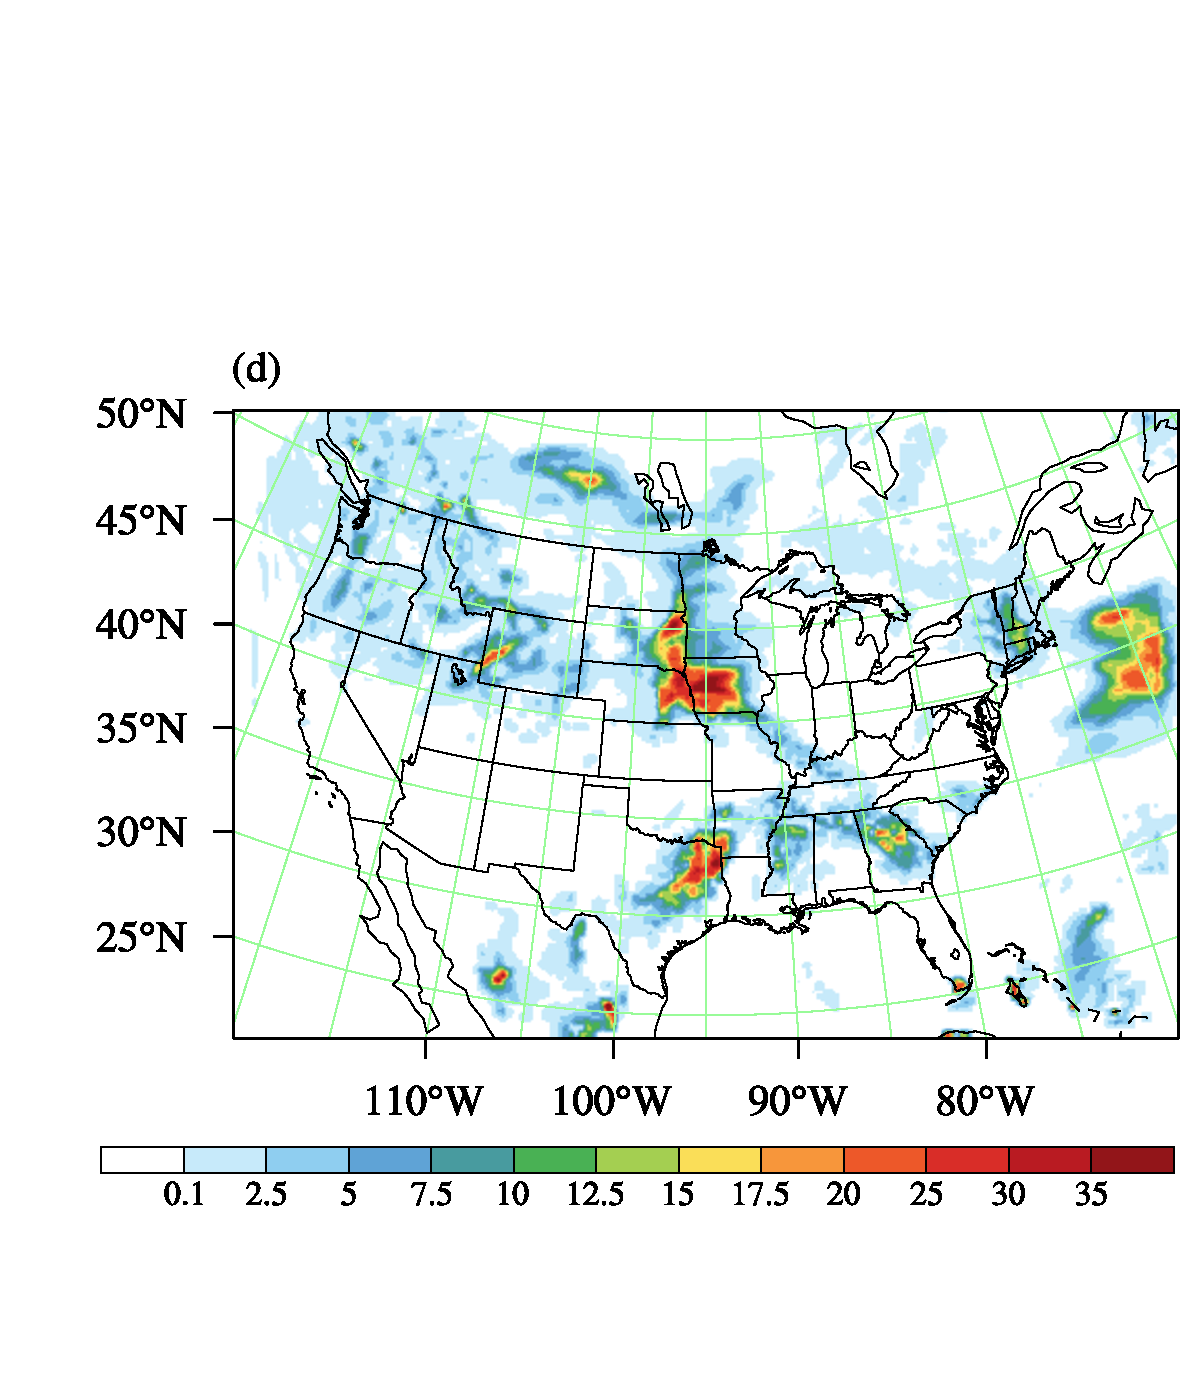
\includegraphics[width=0.4\linewidth]{./figures/gts+rain_copy.pdf}
%\includegraphics[width=0.4\linewidth]{gts+rain.eps}
\caption{12-h accumulated precipitation (mm) from 0000 UTC to 1200 UTC 10 June 2010. (a) NCEP Stage-IV (b) CONTROL (c) GTS (d) GTS+RAIN. }\label{rainfall}
\end{figure}

%\begin{table}
%\caption{Table caption}\label{sampletable}
%\begin{tabular}{l l l}
%\hline
%\textbf{Treatments} & \textbf{Response 1} & \textbf{Response 2}\\
%\hline
%Treatment 1 & 0.0003262 & 0.562 \\
%Treatment 2 & 0.0015681 & 0.910 \\
%Treatment 3 & 0.0009271 & 0.296 \\
%\hline
%\end{tabular}
%\end{table}

\end{document}

%%%%%%%%%%%%%%%%%%%%%%%%%%%%%%%%%%%%%%%%%%%%%%%%%%%%%%%%%%%%%%%

More Information and Advice:

%% ------------------------------------------------------------------------ %%
%
%  SECTION HEADS
%
%% ------------------------------------------------------------------------ %%

% Capitalize the first letter of each word (except for
% prepositions, conjunctions, and articles that are
% three or fewer letters).

% AGU follows standard outline style; therefore, there cannot be a section 1 without
% a section 2, or a section 2.3.1 without a section 2.3.2.
% Please make sure your section numbers are balanced.
% ---------------
% Level 1 head
%
% Use the \section{} command to identify level 1 heads;
% type the appropriate head wording between the curly
% brackets, as shown below.
%
%An example:
%\section{Level 1 Head: Introduction}
%
% ---------------
% Level 2 head
%
% Use the \subsection{} command to identify level 2 heads.
%An example:
%\subsection{Level 2 Head}
%
% ---------------
% Level 3 head
%
% Use the \subsubsection{} command to identify level 3 heads
%An example:
%\subsubsection{Level 3 Head}
%
%---------------
% Level 4 head
%
% Use the \subsubsubsection{} command to identify level 3 heads
% An example:
%\subsubsubsection{Level 4 Head} An example.
%
%% ------------------------------------------------------------------------ %%
%
%  IN-TEXT LISTS
%
%% ------------------------------------------------------------------------ %%
%
% Do not use bulleted lists; enumerated lists are okay.
% \begin{enumerate}
% \item
% \item
% \item
% \end{enumerate}
%
%% ------------------------------------------------------------------------ %%
%
%  EQUATIONS
%
%% ------------------------------------------------------------------------ %%

% Single-line equations are centered.
% Equation arrays will appear left-aligned.

Math coded inside display math mode \[ ...\]
 will not be numbered, e.g.,:
 \[ x^2=y^2 + z^2\]

 Math coded inside \begin{equation} and \end{equation} will
 be automatically numbered, e.g.,:
 \begin{equation}
 x^2=y^2 + z^2
 \end{equation}

% IF YOU HAVE MULTI-LINE EQUATIONS, PLEASE
% BREAK THE EQUATIONS INTO TWO OR MORE LINES
% OF SINGLE COLUMN WIDTH (20 pc, 8.3 cm)
% using double backslashes (\\).

% To create multiline equations, use the
% \begin{eqnarray} and \end{eqnarray} environment
% as demonstrated below.
\begin{eqnarray}
  x_{1} & = & (x - x_{0}) \cos \Theta \nonumber \\
        && + (y - y_{0}) \sin \Theta  \nonumber \\
  y_{1} & = & -(x - x_{0}) \sin \Theta \nonumber \\
        && + (y - y_{0}) \cos \Theta.
\end{eqnarray}

%If you don't want an equation number, use the star form:
%\begin{eqnarray*}...\end{eqnarray*}

% Break each line at a sign of operation
% (+, -, etc.) if possible, with the sign of operation
% on the new line.

% Indent second and subsequent lines to align with the first character following the equal sign on the first line.

% Use an \hspace{} command to insert horizontal space into your equation if necessary. Place an appropriate unit of measure between the curly braces, e.g. \hspace{1in}; you may have to experiment to achieve the correct amount of space.


%% ------------------------------------------------------------------------ %%
%
%  EQUATION NUMBERING: COUNTER
%
%% ------------------------------------------------------------------------ %%

% You may change equation numbering by resetting
% the equation counter or by explicitly numbering
% an equation.

% To explicitly number an equation, type \eqnum{}
% (with the desired number between the brackets)
% after the \begin{equation} or \begin{eqnarray}
% command.  The \eqnum{} command will affect only
% the equation it appears with; LaTeX will number
% any equations appearing later in the manuscript
% according to the equation counter.
%

% If you have a multiline equation that needs only
% one equation number, use a \nonumber command in
% front of the double backslashes (\\) as shown in
% the multiline equation above.

%% ------------------------------------------------------------------------ %%
%
%  SIDEWAYS FIGURE AND TABLE EXAMPLES
%
%% ------------------------------------------------------------------------ %%
%
% For tables and figures, add \usepackage{rotating} to the paper and add the rotating.sty file to the folder.
% AGU prefers the use of {sidewaystable} over {landscapetable} as it causes fewer problems.
%
% \begin{sidewaysfigure}
% \includegraphics[width=20pc]{samplefigure.eps}
% \caption{caption here}
% \label{label_here}
% \end{sidewaysfigure}
%
% \begin{sidewaystable}
% \caption{}
% \begin{tabular}
% Table layout here.
% \end{tabular}
% \end{sidewaystable}